\documentclass[12pt]{report}


% Macro definitions, packages
% linking and coloring
\usepackage{color}   %May be necessary if you want to color links
\usepackage{hyperref}
\hypersetup{
    colorlinks=false, %set true if you want colored links
    linktoc=all,     %set to all if you want both sections and subsections linked
    linkcolor=blue,  %choose some color if you want links to stand out
}

% \usepackage[margin=1in]{geometry}


\usepackage{setspace}
\usepackage{upgreek}
\usepackage{url}
\usepackage{booktabs}
\usepackage{upgreek}
\usepackage{graphicx}
\usepackage{color}
\usepackage{amsmath}
\usepackage{amssymb}
\usepackage{slashed}
\usepackage{mathalfa}
\usepackage{float}
\usepackage{overpic}
\usepackage{afterpage}
\usepackage{pdfpages}


\usepackage[section]{placeins}



\usepackage{physics}
\usepackage{braket} % include after physics
\usepackage{xspace}
\usepackage{siunitx}

\usepackage{multirow}
\usepackage{indentfirst}

\usepackage[margin=1.5cm]{caption}
\usepackage{subcaption}
% \usepackage[splitrule]{footmisc}
\interfootnotelinepenalty=10000



\def\code#1{\texttt{#1}}

\usepackage{dcolumn}
\newcolumntype{d}[1]{D{.}{.}{#1} }
\newcolumntype{C}[1]{>{\centering\arraybackslash}m{#1}}
\usepackage{makecell}

\usepackage{tabularx}



% feynman diagrams
\usepackage{tikz-feynman}
\tikzfeynmanset{compat=1.0.0}
\usepackage{rotating}


\newcommand*{\titleName}{Searches for the rare decay of the Higgs boson to two muons and for new physics in dilepton final states with the ATLAS Experiment}

% particles
\newcommand*{\pp}{\ensuremath{pp}\xspace}
\newcommand*{\mm}{\ensuremath{\mu\mu}\xspace}
\newcommand*{\tautau}{\ensuremath{\tau\tau}\xspace}
\newcommand*{\ee}{\ensuremath{ee}\xspace}
\let\llt\ll % booya!
\renewcommand*{\ll}{\ensuremath{\ell\ell}\xspace}
\newcommand*{\W}{\ensuremath{W^\pm}\xspace}
\newcommand*{\Wp}{\ensuremath{W^+}\xspace}
\newcommand*{\Wm}{\ensuremath{W^-}\xspace}
\newcommand*{\Z}{\ensuremath{Z}\xspace}
\newcommand*{\jpsi}{\ensuremath{J/\psi}\xspace}
\newcommand*{\vhmm}{\ensuremath{V(H\to\mu\mu)}\xspace}
\newcommand*{\mh}{\ensuremath{m_{H}}\xspace}
\newcommand*{\muu}{\ensuremath{m_{\mu\mu}}\xspace}
\newcommand*{\mee}{\ensuremath{m_{ee}}\xspace}
\newcommand*{\mll}{\ensuremath{m_{\ell\ell}}\xspace}
\newcommand*{\qqll}{\ensuremath{q\overline{q}\ell^+\ell^-}\xspace}
\newcommand*{\llqq}{\ensuremath{\qqll}\xspace}
\newcommand*{\e}{\ensuremath{e}\xspace}
\newcommand*{\m}{\ensuremath{\mu}\xspace}
\newcommand*{\h}{\ensuremath{H}\xspace}
\newcommand*{\pt}{\ensuremath{p_\text{T}}\xspace}
\newcommand*{\plong}{\ensuremath{p_\text{L}}\xspace}
\newcommand*{\httt}{\ensuremath{H_\text{T}}\xspace}
\newcommand*{\et}{\ensuremath{E_\text{T}}\xspace}
\newcommand*{\met}{\ensuremath{E_T^\mathrm{miss}}\xspace}
\newcommand*{\sqrts}{\ensuremath{\sqrt{s}}\xspace}
\newcommand*{\sqrths}{\ensuremath{\sqrt{\hat{s}}}\xspace}

% chiralities
\newcommand*{\fl}{\ensuremath{f_\text{L}}\xspace}
\newcommand*{\fr}{\ensuremath{f_\text{R}}\xspace}
\newcommand*{\flp}{\ensuremath{f'_\text{L}}\xspace}
\newcommand*{\frp}{\ensuremath{f'_\text{R}}\xspace}
\newcommand*{\ufl}{\ensuremath{\overline{f}_\text{L}}\xspace}
\newcommand*{\ufr}{\ensuremath{\overline{f}_\text{R}}\xspace}
\newcommand*{\uflp}{\ensuremath{\overline{f}'_\text{L}}\xspace}
\newcommand*{\ufrp}{\ensuremath{\overline{f}'_\text{R}}\xspace}

% mandelstram
\newcommand*{\shat}{\ensuremath{\hat{s}}\xspace}
\newcommand*{\uhat}{\ensuremath{\hat{u}}\xspace}
\newcommand*{\that}{\ensuremath{\hat{t}}\xspace}
\newcommand*{\qbar}{\ensuremath{\overline{q}}\xspace}
\newcommand*{\ubar}{\ensuremath{\overline{u}}\xspace}
\newcommand*{\dbar}{\ensuremath{\overline{d}}\xspace}
\newcommand*{\pbar}{\ensuremath{\overline{p}}\xspace}
\newcommand*{\fbar}{\ensuremath{\overline{f}}\xspace}
\newcommand*{\tbar}{\ensuremath{\overline{t}}\xspace}
\newcommand*{\bbar}{\ensuremath{\overline{b}}\xspace}
\newcommand*{\cbar}{\ensuremath{\overline{c}}\xspace}

\newcommand*{\neutralcone}{\ensuremath{\pt^\text{neu20}}\xspace}
\newcommand*{\ptcone}{\ensuremath{\pt^\text{cone20}}\xspace}
\newcommand*{\ptvarconeMuon}{\ensuremath{\pt^\text{varcone30}}\xspace}
\newcommand*{\ptvarconeElec}{\ensuremath{\pt^\text{varcone20}}\xspace}
\newcommand*{\etcone}{\ensuremath{\et^\text{topocone20}}\xspace}
\newcommand*{\xsbr}{\ensuremath{\sigma_\text{visible}\times\text{BR}}\xspace}
\newcommand*{\acceff}{\ensuremath{\mathcal{A}\times\epsilon_\text{sig}}\xspace}
\newcommand*{\lam}{\ensuremath{\Lambda}\xspace}
\newcommand*{\nsig}{\ensuremath{N_\text{sig}}\xspace}
\newcommand*{\nbkg}{\ensuremath{N_\text{bkg}}\xspace}

% Generators
\newcommand*{\powheg}{\textsc{Powheg-Box}\xspace}
\newcommand*{\sherpa}{\textsc{Sherpa}\xspace}
\newcommand*{\madgraph}{\textsc{MadGraph5}\_aMC@NLO\xspace}
\newcommand*{\pythia}{\textsc{Pythia}\xspace}
\newcommand*{\evtgen}{\textsc{EvtGen}\xspace}
\newcommand*{\geant}{\textsc{Geant}\xspace}
\newcommand*{\xgb}{\textsc{XGBoost}\xspace}
\newcommand*{\etal}{\emph{et~al.}\xspace}




% statistics
\newcommand*{\cls}{\ensuremath{\text{CL}_\text{s}}\xspace}
\newcommand*{\clb}{\ensuremath{\text{CL}_\text{b}}\xspace}
\newcommand*{\clsb}{\ensuremath{\text{CL}_\text{s+b}}\xspace}
\newcommand*{\mus}{\ensuremath{\mu_\text{S}}\xspace}
\newcommand*{\nss}{\ensuremath{N_\text{ss}}\xspace}

% processes
\newcommand*{\hmm}{\ensuremath{H\to\mm}\xspace}
\newcommand*{\nr}{\ensuremath{non-resonant}\xspace}

% units
\newcommand*{\cms}{\ensuremath{\text{cm}^{-2}\text{s}^{-1}}\xspace}
\newcommand*{\fb}{\ensuremath{\text{fb}^{-1}}\xspace}
\newcommand*{\um}{\ensuremath{\mu\text{m}}\xspace}
\newcommand*{\us}{\ensuremath{\mu\text{s}}\xspace}

% variables

\newcommand*{\half}{\ensuremath{\frac{1}{2}}\xspace}
\newcommand*{\as}{\ensuremath{\alpha_s\xspace}}
\newcommand*{\reals}{\ensuremath{\mathbb{R}}\xspace}
\newcommand*{\ident}{\ensuremath{\mathbb{I}}\xspace}
\newcommand*{\nxn}{\ensuremath{n\times n}\xspace}

\newcommand*{\vtheta}{\ensuremath{\vec{\theta}}\xspace}
\newcommand*{\poincare}{Poincar\^e\xspace}
\renewcommand*{\check}{{\color{red}[check]}\xspace}


\usepackage[utf8]{inputenc}
\usepackage[T1]{fontenc}
\usepackage{lmodern}
% \usepackage[showframe, textwidth = 15cm, nomarginpar, noheadfoot]{geometry}
\usepackage{mathtools}
\newcommand{\shortnote}[1]{ &  & \text{\small\llap{#1}}}
\newcommand{\longeqnote}[1]{& & \\ \notag  &  &  &  &  & \text{\small\llap{#1}}}

\newcommand{\centered}[1]{\begin{tabular}{l} #1 \end{tabular}}



\newcommand*{\POWHEG}{\textsc{Powheg}\xspace}
\newcommand*{\POWHEGV}[1]{\textsc{Powheg}~#1\xspace}
\newcommand*{\POWHEGBOX}{\textsc{Powheg-Box}\xspace}
\newcommand*{\POWHEGBOXV}[1]{\textsc{Powheg-Box}~#1\xspace}
\newcommand*{\PYTHIA}{\textsc{Pythia}\xspace}
\newcommand*{\PYTHIAV}[1]{\textsc{Pythia}~#1\xspace}
\newcommand*{\SHERPA}{\textsc{Sherpa}\xspace}
\newcommand*{\SHERPAV}[1]{\textsc{Sherpa}~#1\xspace}
\newcommand*{\GEANT}{\textsc{Geant}\xspace}



% ############################################################
% Commands for Ensemble Appendix
% ############################################################
\newcommand*{\spur}{\ensuremath{\sigma^\mathrm{spur}}\xspace}
\newcommand*{\func}{\ensuremath{f(\mll)}\xspace}
\newcommand*{\truth}{\ensuremath{f^\mathrm{truth}(\mll)}\xspace}
\newcommand*{\realsBkg}{\ensuremath{\mathbb{R}^{\dbkg}}\xspace}
\newcommand*{\realsSyst}{\ensuremath{\mathbb{R}^{\dsyst}}\xspace}
\newcommand*{\eeReal}{\ensuremath{\mathbb{R}}\xspace}
\newcommand*{\map}{\ensuremath{h(\realsBkg)\mapsto\eeReal}\xspace}
% mapping theta->bkg shape
\newcommand*{\mapThetaToBkg}{\ensuremath{g(\nps|\systs)\mapsto\realsBkg}\xspace}
\newcommand*{\thetaToBkg}{\ensuremath{g(\nps|\systs)}\xspace}
\newcommand*{\eeDd}{\ensuremath{\Delta}\xspace}
\newcommand*{\deltaTheta}{\ensuremath{\Delta^\theta}\xspace}
\newcommand*{\deltaD}{\ensuremath{\Delta^D}\xspace}
\newcommand*{\deltaDSquared}{\ensuremath{(\Delta^D)^2}\xspace}
\newcommand*{\deltaThetaSquared}{\ensuremath{(\Delta^\theta)^2}\xspace}
\newcommand*{\np}{\ensuremath{\theta_i}\xspace}
\newcommand*{\npmeasured}{\ensuremath{\hat{\theta_i}}\xspace}
\newcommand*{\npprob}{\ensuremath{G(\theta_i)}\xspace}
\newcommand*{\nps}{\ensuremath{\vec{\theta}}\xspace}
% Dimensions
\newcommand*{\ddata}{\ensuremath{N_\mathrm{data}}\xspace}
\newcommand*{\dbkg}{\ensuremath{N_\mathrm{bkg}}\xspace}
\newcommand*{\dsyst}{\ensuremath{N_\mathrm{syst}}\xspace}
% mean and std
\newcommand*{\meanD}{\ensuremath{\mathrm{E}[\deltaD]}\xspace}
\newcommand*{\meanDSquared}{\ensuremath{\mathrm{E}[(\deltaD)^2]}\xspace}
\newcommand*{\meanTheta}{\ensuremath{\mathrm{E}[\deltaTheta]}\xspace}
\newcommand*{\meanThetaSquared}{\ensuremath{\mathrm{E}[(\deltaTheta)^2]}\xspace}
\newcommand*{\stdD}{\ensuremath{\mathrm{var}[\deltaD]}\xspace}
\newcommand*{\stdTheta}{\ensuremath{\mathrm{var}[\deltaTheta]}\xspace}
% # datasets
\newcommand*{\template}{\ensuremath{\vec{D}}\xspace}
\newcommand*{\mc}{\ensuremath{\vec{D}^\mathrm{MC}}\xspace}
\newcommand*{\data}{\ensuremath{\vec{D}^\mathrm{data}}\xspace}
\newcommand*{\truthdata}{\ensuremath{\vec{D}^\mathrm{truth}}\xspace}
\newcommand*{\truthguess}{\ensuremath{\vec{X}^\mathrm{truth}}\xspace}
\newcommand*{\syst}{\ensuremath{\vec{D}^\mathrm{syst}_i}\xspace}
\newcommand*{\systUp}{\ensuremath{\vec{D}^\mathrm{+syst}_i}\xspace}
\newcommand*{\systDn}{\ensuremath{\vec{D}^\mathrm{-syst}_i}\xspace}
\newcommand*{\systs}{\ensuremath{\{\vec{D}^\mathrm{syst}\}}\xspace}
% analysis functions
\newcommand*{\eeNbkg}{\ensuremath{F(\vec{D})}\xspace}
\newcommand*{\nbkgmc}{\ensuremath{F(\mc)}\xspace}
\newcommand*{\nbkgdata}{\ensuremath{F(\data)}\xspace}
\newcommand*{\nbkgtruth}{\ensuremath{F(\truthdata)}\xspace}

\newcommand*{\gsm}{\ensuremath{\text{G}_\text{SM}}\xspace}



% Bib info
\usepackage{cite}
% \addbibresource{resources.bib}
% \usepackage[margin=0.7in]{geometry} % 1in for Umich
\usepackage[margin=1.0in]{geometry} % 1in for Umich
\setcounter{errorcontextlines}{50}

\title{\titleName}
\author{Aaron White}

% \setstretch{0.9} % 1.5 for Umich
\onehalfspacing

\nonstopmode

\begin{document}

\pagenumbering{gobble}
\begin{titlepage}

\begin{center}
\phantom{x}\\
\vspace{10em}
\textbf{\Large\titleName}\\
\vspace{5em}
by\\
Aaron White\\
\vspace{5em}
A dissertation submitted in partial fulfillment\\
of the requirements for the degree of\\
Doctor of Philosophy\\
(Physics)\\
in The University of Michigan\\
2020\\
\end{center} 

\vspace{5em}
\noindent Doctoral Comittee:\\
\phantom{xxxx} Professor Bing Zhou, Chair \\
\phantom{xxxx} Professor Tom Schwarz\\
\phantom{xxxx} Professor Christine Aidala\\
\phantom{xxxx} Professor James Wells\\
\phantom{xxxx} Professor David Baker\\

\end{titlepage}


\tableofcontents

\pagenumbering{Roman}
\cleardoublepage
\addcontentsline{toc}{chapter}{Acknowledgements}
\begin{center}
\textbf{\LARGE Acknowledgements}
\end{center} 

During my time working on this project, I have benefitted from the help and generosity of many people.
I would like to thank the members the ATLAS Collaboration who have built and run the detector and computing infrastructure that has enabled my work.
I would also like to thank the enginners and staff at CERN who help operate the LHC and maintian the site.
I am thankful to the Michigan professors Junjie Zhu, Jianming Qian, Homer Neal, and Jay Chapman for building a supportive university environment.
I am thankful to the many friends I have made with for engaging in interesting discussions, especially Tom Cheng, Yicheng Guo, Zhi Zheng, Zirui Wang, Rongkun Wang, Zhongyukun Xu, and Siyuan Sun, Yanlin Liu, Hao Liu, and Dan Marley.
In particular, Matthew Klein has provided patient and invaluable supervision on topics of data analysis.
During my authorship qualification, I benifitted from the guidance of Tom Schwarz and technical instruction of Xueye Hu, Jinhong Wang, and Bob Ball.
On the search for the Higgs decay to two muons, I am thankful for the guidance of guidance of Yusheng Wu, Yanlin Liu, and Bing Li.
On the search for contact interactions, I would like to thank the Exotics-LPX Dilepton group and our ever patient editorial board, Paul de Jong, Ulla Blumenschein, and Elliot Lipelles for their feedback.
I would especially like to thank Uta Klein, Dan Hayden, Etienne Dreyer, Peter Falke, Tanya Hryn'Ova, Sean Lawler for their contributions and guidance.
I am thankful for the LPX and Exotics group leadership of Yasu Okumura, Nikolina Llic, Antonio Sidoti, Carl Gwilliam, and Oliver Stelzer-Chilton.
Penultimately, I want to note my great fortune in working on this project with Deshan Abhayasinghe and Noam Tal Hod, who have made the this project one of the highlights of the past five years..
Finally, I want to my deepest thanks to my advisor, Bing Zhou.
She has worked tirelessly to support me since, as an undergraduate, I enrolled in her section of Physics 405: Intermediate Electromagnitism.
As a role model, her presistant curiosity and attention to detail have provided an exceptional example of an experimental physicist. 
As a mentor, she has always pushed me to be better.



\cleardoublepage
\addcontentsline{toc}{chapter}{List of Figures}
\listoffigures
\cleardoublepage
\addcontentsline{toc}{chapter}{List of Tables}
\listoftables
\cleardoublepage
\addcontentsline{toc}{chapter}{Abstract}
\begin{center}
\textbf{\LARGE Abstract}
\end{center} 

This thesis presents a search for rare dimuon decay of the Higgs boson and a search for new physics with non-resonant phenomena at the TeV mass scale with dilepton final states.  Both studies use data, corresponding to an integrated luminosity of 139~fb$^{1}$, recorded by the ATLAS experiment in proton--proton collisions at a centre-of-mass energy of $\sqrt{s}=13$~TeV during Run~2 of the Large Hadron Collider.

The detection of the Standard Model $H\to\mu\mu$ decay is important to study the Higgs boson Yukawa couplings to the 2nd generation fermions.
Detecting the signal of Higgs boson decay to dimuon is extremely challenging due to the small decay branching fraction ($2.
2\times10^{-4}$) and large irreducible background from Drell-Yan production.
To increase the detection sensitivity, multiple event selection categories are developed based on the Higgs production modes and final state event topologies.
The major Higgs production modes at the LHC are gluon-gluon fusion (ggF), vector-boson fusion (VBF), a vector boson (W or Z) associated production (VH), and a top pair associated production (ttH).
Much of the focus of this thesis revolves around selecting VH events with different lepton final states.
The final state topologies include different jet multiplicity, and different lepton multiplicity, as well as b-jet tagging.
Machine-learning multivariate analysis (MVA) methods are developed and implemented to select events for different categories.
Background expectations are determined from the side-band events of the dimuon invariant mass spectra.
A statistic model is developed to combine events selected in different categories to extract the Higgs signal strength.
The limits set on signal production in the new phase spaces explored in this analysis are the first of their kind.
The strongest expected (observed) limit on leptonic VH production excludes signals down to 13.2(22.6) times the Standard Model prediction.
The combination of VH with the other major production modes results in a signal significance of 2.0$\sigma$.

To explore the quark and lepton internal structure, a search for new physics in the context of contact-interactions (CI) with non-resonant signals in dielectron and dimuon invariant mass spectra in the multi-TeV mass range is performed.
The experimental signal of the underlying physics would enhance the dilepton event rate at the TeV mass scale.
The major background is the dilepton from the Drell-Yan process.
A functional form is fit to the data to model the background.
This is done in a low-mass control region where the signal is expected to be negligible, while the function is extrapolated to several high-mass signal regions where an enhancement of events is expected above the background processes.
This is a novel approach at the LHC, which overcomes the limitations of both statistical and systematical uncertainties by using Monte Carlo events to estimate the background contribution.
In this search, no significant deviation in data is observed with respect to the expected background.
Upper limits on the visible cross-section times branching ratio are set in this search.
These, along with benchmark CI signal efficiencies, can be interpreted as limits in terms of a variety of signal models.
The lower limits on the energy scale of CI, $\Lambda$, reaches 35.8 TeV, indicating the quarks and leptons are still point-like particles at 10$^{-20}$ m.
These are the strongest limits on $q\bar{q}\ell^+\ell^-$ contact-interactions to date.



\pagenumbering{arabic}


\chapter{Introduction}

\mm \pp


% History

\chapter{Theory}

\section{Standard Model}
\section{Electroweak Symmetry Breaking}
\section{Contact Interactions}

\chapter{Experimental Apaparatus} 

\section{CERN Accelerator Complex}
\section{Large Hadron Collider}

\section{ATLAS Detector}
\subsection{Magnet System}
\subsection{Inner Detector}
\subsection{Calorimeters}
\subsection{Muon System}
\subsection{Trigger System}
\subsection{Event Reconstruciton}


\chapter{Phenomenology}\label{sec:phenomenology}

\section{Physics at Hadron Colliders}

The LHC collides protons together in order to create collisions with center-of-mass-energy \sqrts.
During a collision, the protons' constituents may interact directly and exchange a substantial fraction of their proton's momentum, in a process called hard-scattering.
These interactions may be quark-quark, quark-gluon, or gluon-gluon scattering events that can be described with a degree of fidelity by a matrix element complication.
This is a messy process and is complicated by the composite nature of the protons.
This section describes how colliding protons may produce events that are of interest to this thesis.

\subsection{Parton distribution function}

\begin{figure}[h!]
\captionsetup[subfigure]{position=b}
\centering
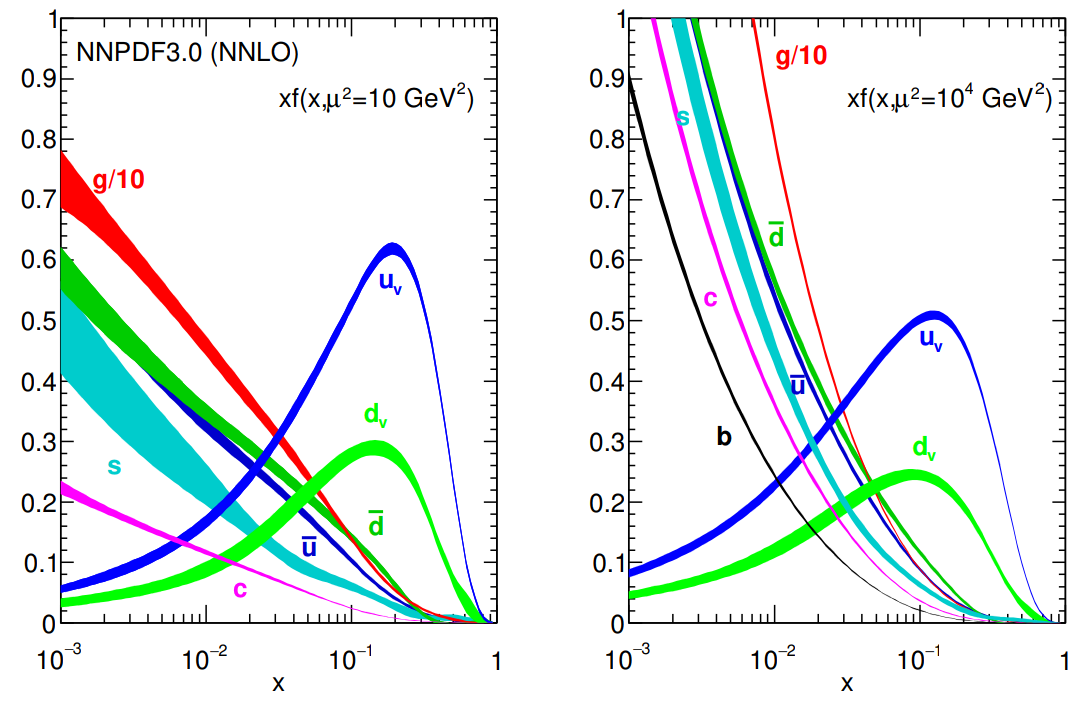
\includegraphics[width=0.99\textwidth]{figures/pheno/pdgpdf.png}
\caption{Parton distribution functions $xf_i(x,Q)$ calculated using NNPDF3.0 with energy scale $Q^2=10\text{~GeV}^2$ (left) and $Q^2=10^4\text{~GeV}^2$ (right). This figure is from \cite{Ball:2014uwa}.}
\label{fig:partDistFunc}
\end{figure}

The protons that make up the colliding beams at the LHC are bound states of quarks and gluons, collectively called partons.
These consist of three valance quarks ($uud$), and a \emph{sea} or virtual quark/anti-quark pairs.
When two protons collide with sufficient energy \footnote{On the scale of $\Lambda_\text{QCD}\approx218$~MeV.}, two types of qualitative processes take place.
First is \emph{hard-scattering}, an interaction mediated by a large momentum exchange between typically two partons.
Second is \emph{soft-scattering}, where the remaining partons interact through the low energy mediators.
While both processes are interesting, hard-scattering interactions are of particular interest in this thesis, as these provide access to particularly high energy interactions.

When two partons interact, each carries a fraction of their respective proton's total energy \sqrts.
The longitudinal component of the momentum fraction is termed Feynman's $x$.
When a high energy probe particle collides with a proton, the probe will hard-scatter off of one of the proton's constituents, be it a quark or gluon.
In $pp$ collisions, the probe is a parton selected from a proton in the opposing beam.
The probability of the probe to scatter off a particular parton $i$ depends both on its momentum fraction $x$ and on the momentum exchange $Q$.
This differential probability function, $f_i(x,Q)$, is called the parton distribution function (PDF).
Hence, $f_u(x,Q)$ gives the that the probe will interact with an up quark, while $f_{\overline{s}}(x,Q)$ gives the corresponding probability for an interaction with an anti-strange quark.

The proton dynamics that determine PDFs occur at low $Q$, where calculations are complicated by the large QCD coupling from Equation \ref{eqn:alphas}.
Instead of analytic calculations, PDFs functions are fit to experimental measurements.
The resulting PDF shapes as a function of $x$ is shown in Figure \ref{fig:partDistFunc} for each parton.
The valance quarks ($u$ and $d$) are seen to have probability peaks between $x=0.1$ and $x=0.2$, indicating a relatively high frequency that these carry a large portion of the proton's momentum.
In contrast, the sea quarks ($\overline{u}$, $\overline{d}$, $s/\overline{s}$, and $c/\overline{c}$) typically carry a much smaller momentum fraction.
The $u$ and $d$ quarks contribute to the sea as well, and Figure \ref{fig:partDistFunc} separates the valance component from the sea component for these.
The PDFs of the sea $u$ and $d$ quarks and anti-quarks are identical since these are produced in virtual pairs.
The PDFs for gluons are shown scaled down by a factor of 10, as nearly half the proton's momentum is carried by gluons.\cite{wells}

The differential cross sections of an $2\to X$ interaction, given in Equation \ref{eqn:diffCrossSection}, depend on the initial state particles.
When two protons collide, the initial state particles of a hard-scattering process are selected randomly from each proton according to the parton distribution functions.
Consequently, the total cross-section of a $pp$ collision corresponds to a sum over partons $i,j$ in each proton, respectively, and an integral over momentum fractions.
The $pp$ version of the differential cross section is given in Equation \ref{eqn:ppDiffCrossSection}.
\begin{equation}\begin{split}\label{eqn:ppDiffCrossSection}
d\sigma(pp\to X)=\sum_i\sum_j\int_0^1dx_i\int_0^1dx_j~d\sigma(ij\to X)f_i(x_i)f_j(x_j)
\end{split}\end{equation} 
This sum tallies the cross sections $d\sigma(ij\to X)$ for each possible configuration of initial states, weighted by the likelihood of the initial state $ij$.

\subsection{Parton Luminosity}

\begin{figure}[h!]
\captionsetup[subfigure]{position=b}
\centering
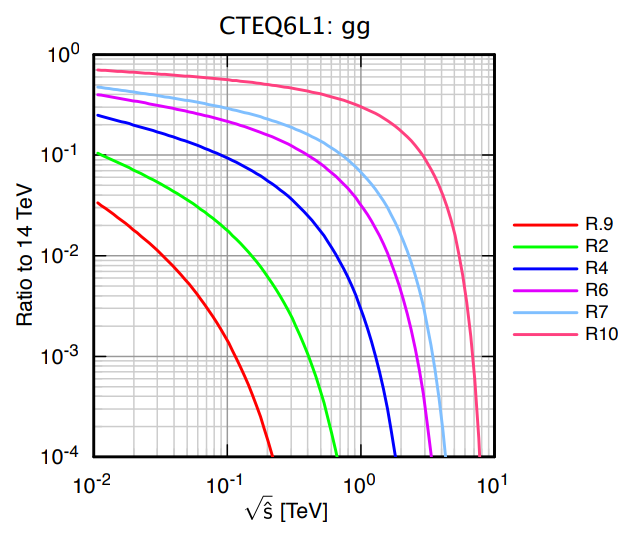
\includegraphics[width=0.5\textwidth]{figures/pheno/partonLumi.png}
\caption{Comparison of $gg$ luminosity for different \sqrts, plotted as a ratio to the luminosity at \sqrts=14~TeV. Figure from \cite{quigg}.}
\label{fig:partonLumi}
\end{figure}

The luminosity defined in Equation \ref{eqn:lumi} is defined in terms of the $pp$ cross section $\sigma_{pp}$.
A more specific \emph{parton luminosity} $\mathcal{L}_{ij}$ may be defined for particular species of parton $i$ and $j$ with center of mass energy $\sqrths<\sqrts$.
The ``hatted'' variables correspond to values in the parton's center of mass frame.
\begin{equation}\begin{split}\label{eqn:partonLumi}
\frac{\tau}{\shat}\frac{d\mathcal{L}_{ij}}{d\tau}\equiv\frac{\tau}{\shat(1+\delta_{ij})} \int_\tau^1 \frac{dx}{x}~f_i(x)f_j(\tau/x)+f_j(x)f_i(\tau/x)]
\end{split}\end{equation}
This definition supposes the beam consists of partons rather than protons, and each parton combination has an associated luminosity that is a function of the fraction $\tau=\shat/s$.
This luminosity is seen to depend on the beam energy through the presence of the PDFs and Feynman's $x$.
The total cross section for $pp\to X$ is defined by with a sum over parton species,
\begin{equation}\begin{split}
\sigma_{pp\to X}(s)=\sum_i\sum_j \frac{d\tau}{\tau}\cdot\frac{\tau}{\shat}\frac{d\mathcal{L}_{ij}}{d\tau}\cdot[\shat\sigma_{ij\to X}(\shat)].
\end{split}\end{equation} 
As indicated by the shapes of PDF curves, the parton luminosity for a beam of energy \sqrts drops off as a function of \sqrths.
\cite{quigg}

Consequently, although the LHC collides beams with \sqrts=13~TeV, the practical luminosity of collisions with \sqrths=13~TeV essentially vanishes.
This limits the energy available in hard scattering to a fraction of \sqrts.
For example, the invariant-mass of the most energetic two-jet event recorded by ATLAS in Run~2 is just $m_{jj}=8$~TeV.
A second consequence of Equation \ref{eqn:partonLumi} arises from its dependence on the proton center of mass energy \sqrts (through $\tau$).
Increasing the \sqrts greatly expands the parton luminosity at large \sqrths.
Both of these effects are illustrated in Figure \ref{fig:partonLumi}, which plots the ratio of $gg$ parton luminosities at the different center-of-mass energies to the LHC design value.

\section{Standard Model Dilepton Production}\label{sec:phenoBkg}

Both the \hmm search and the non-resonant search share a similar interest in the dilepton invariant mass spectra.
As such, the backgrounds for these analyses share a similar composition produced by standard model processes.
The dominant hard-scattering processes that produce events with dilepton pairs in the high invariant-mass region at the LHC are described in this section.

\begin{figure}[h!]
\captionsetup[subfigure]{position=b}
\centering
    \feynmandiagram [medium,baseline=(v1.base),horizontal=v1 to v2] {
    q1[particle=\(q\)] --[fermion] v1 --[boson,edge label=\(\gamma^*/Z\)] v2 --[fermion] z1[particle=\(\ell^-\)],
    v1 --[fermion] q2[particle=\(\overline{q}\)],
    z2[particle=\(\ell^+\)] --[fermion]v2,
    }; \\ [1em]
\caption{Feynman diagram for the leading order Drell-Yan process.}
\label{fig:phenoDy}
\end{figure}

The most significant lepton pair production mechanism in hadronic collisions was proposed in 1970 by Sidney Drell and Tung-Mow Yan. 
The process is described as the annihilation of partons from opposing protons to produce a massive intermediate state that carries the momentum exchange of the collision. \cite{drellYan}
For collision energies below the \Z mass, this intermediate state is an off-shell photon.
Above the \Z mass, both photons and \Z bosons mediate Drell-Yan production, as illustrated in Figure \ref{fig:phenoDy}.
The predicted differential cross-section falls sharply as the produced dilepton pair's invariant mass grows.
Although this prediction is inaccurate near the \Z mass where resonant production dominates, in the kinematic regions of interest for this thesis, it describes the background to first order.

\begin{figure}[h!]
\captionsetup[subfigure]{position=b}
\centering
\subfloat[][]{{
    \feynmandiagram [medium,baseline=(v1.base),vertical=v2 to v1] {
    b[particle=\(q\)] --[fermion] v2,
    v2 --[boson] t[particle=\(Z\)],
    v1 --[boson] qb[particle=\(Z\)],
    v1 --[fermion] qa[particle=\(\overline{q}'\)],
    v2 --[fermion] v1,
    };
}}
\hspace{2em}
\subfloat[][]{{
    \feynmandiagram [medium,baseline=(v1.base),horizontal=v1 to v2] {
    q1[particle=\(q\)] --[fermion] v1 --[boson,edge label=\(W\)] v2 --[boson] z1[particle=\(Z\)],
    v1 --[fermion] q2[particle=\(\overline{q}'\)],
    v2 --[boson] z2[particle=\(W\)],
    };
}}
\subfloat[][]{{
    \feynmandiagram [medium,baseline=(v1.base),horizontal=v1 to v2] {
    q1[particle=\(q\)] --[fermion] v1 --[boson,edge label=\(Z\)] v2 --[boson] z1[particle=\(W^-\)],
    v1 --[fermion] q2[particle=\(\overline{q}\)],
    v2 --[boson] z2[particle=\(W^+\)],
    };
}}
\caption{Representative Feynman diagrams for leading order diboson production for ZZ (a) WZ (b) and WW (c). \check}
\label{fig:phenoDiboson}
\end{figure}

The next leading source of dilepton events come from \emph{diboson} production.
These are described by diagrams, including those in Figure \ref{fig:phenoDiboson}, with two vector bosons \W or \Z in their final state.
The leading order production of these events is through the $q\qbar$ initial state.

\begin{figure}[h!]
\captionsetup[subfigure]{position=b}
\centering
\subfloat[][]{{
    \feynmandiagram [medium,baseline=(v1.base),horizontal=v1 to v2] {
    b[particle=\(g\)] --[gluon] v1  --[gluon] v2,
    v2 --[fermion] t[particle=\(t\)],
    qa[particle=\(g\)]--[gluon]v1,
    qb[particle=\(\overline{t}\)]--[fermion]v2,
    };
}}
\hspace{2em}
\subfloat[][]{{
    \feynmandiagram [medium,baseline=(v1.base),vertical=v1 to v2] {
    g1[particle=\(g\)] --[gluon] v1,
    t1[particle=\(\overline{t}\)] --[fermion]v1,
    g2[particle=\(g\)] --[gluon] v2 --[fermion] t2[particle=\(t\)],
    v1 --[fermion] v2,
    };
}}
\hspace{2em}
\subfloat[][]{{
    \feynmandiagram [medium,baseline=(v1.base),horizontal=v1 to v2] {
    b[particle=\(q\)] --[fermion] v1  --[gluon] v2,
    v2 --[fermion] t[particle=\(t\)],
    v1--[fermion]qa[particle=\(\overline{q}\)],
    qb[particle=\(\overline{t}\)]--[fermion]v2,
    };
}}
\caption{Representative Feynman diagrams for leading order $t\tbar$ production.}
\label{fig:phenoTtbar}
\end{figure}

\begin{figure}[h!]
\captionsetup[subfigure]{position=b}
\centering
\subfloat[][]{{
    \feynmandiagram [small,baseline=(v1.base),horizontal=qa to qb] {b[particle=\(q\)] --[fermion] v2 --[fermion] t[particle=\(q'\)],qa[particle=\(b\)] --[fermion] v1 --[fermion] qb[particle=\(t\)],v2 --[boson] v1};
}}
\hspace{2em}
\subfloat[][]{{
    \feynmandiagram [small,baseline=(v1.base),horizontal=v1 to v2] {
    b[particle=\(q\)] --[fermion] v1  --[boson,edge label=\(W\)] v2,
    v2 --[fermion] t[particle=\(t\)],
    v1--[fermion]qa[particle=\(\overline{q}'\)],
    qb[particle=\(\overline{b}\)]--[fermion]v2,
    };
}}
\hspace{2em}
\subfloat[][]{{
    \feynmandiagram [small,baseline=(v1.base),horizontal=v1 to v2] {
    b[particle=\(g\)] --[gluon] v1  --[fermion] v2,
    v2 --[fermion] t[particle=\(t\)],
    qa[particle=\(b\)]--[fermion]v1,
    qb[particle=\(W\)]--[boson]v2,
    };
}}
\hspace{2em}
\subfloat[][]{{
    \feynmandiagram [small,baseline=(v1.base),vertical=v1 to v2] {
    b[particle=\(b\)] --[fermion] v1 --[boson] w[particle=\(W\)],
    g[particle=\(g\)] --[gluon] v2 --[fermion] t[particle=\(t\)],
    v1 --[fermion] v2,
    };
}}
\caption{Representative Feynman diagrams for leading order single-top production. Subfigures (a) and (b) show $s$-channel and $t$-channel diagrams respectively. Subfigures (c) and (d) show the leading order $bg\to Wt$ diagrams.}
\label{fig:phenoSingleTop}
\end{figure}

Figure \ref{fig:phenoTtbar} lists diagrams for the production of pairs of top quarks: $t\tbar$.
The leading order diagrams produce top quarks through interactions with gluons.
Figure \ref{fig:phenoSingleTop} shows diagrams for single-top production.
This primarily takes place through production with a lighter quark.
At the LHC, the $t$-channel production shown in Figure \ref{fig:phenoSingleTop} (b) is most prevalent, since the $s$-channel diagram requires a bottom quark initial state. \cite{Kidonakis:2011wy}
Additional production exists in conjunction with a \W boson, which also requires an initial state bottom quark. \cite{Kidonakis:2010ux}
After being produced, the top quarks rapidly decay to a \W and lighter quark (bottom, strange, or down) final state.
Most ($96\pm3\%$) top quarks decay to a final state with a bottom quark. \cite{pdg2018}
The result is, in some cases, a final state with multiple leptons.

\cite{Kidonakis:2011wy, Kidonakis:2010ux}



% \afterpage{
% \begin{table}[htp]
% \begin{center}
% \begin{tabular}{C{0.3\textwidth} C{0.5\textwidth}}
% \toprule
% Process & Diagram \\
% \midrule
% Drell-Yan & 
%     \feynmandiagram [medium,baseline=(v1.base),horizontal=v1 to v2] {
%     q1[particle=\(q\)] --[fermion] v1 --[boson,edge label=\(\gamma^*/Z\)] v2 --[fermion] z1[particle=\(\ell^-\)],
%     v1 --[fermion] q2[particle=\(\overline{q}\)],
%     z2[particle=\(\ell^+\)] --[fermion]v2,
%     }; \\ [1em]
% Diboson &
%     \feynmandiagram [medium,baseline=(v1.base),horizontal=v1 to v2] {
%     q1[particle=\(q\)] --[fermion] v1 --[boson] v2 --[boson] z1[],
%     v1 --[fermion] q2[particle=\(\overline{q}'\)],
%     v2 --[boson] z2[],
%     }; \\ [1em]
% Single-top & 
%     \feynmandiagram [medium,baseline=(v1.base),horizontal=v1 to v2] {
%     b[particle=\(q\)] --[fermion] v1  --[boson,edge label=\(W\)] v2,
%     v2 --[fermion] t[particle=\(\overline{t}\)],
%     v1--[fermion]qa[particle=\(\overline{q}'\)],
%     qb[particle=\(b\)]--[fermion]v2,
%     }; \\ [1em]
% Wt & 
%     \feynmandiagram [medium,baseline=(v1.base),horizontal=v1 to v2] {
%     b[particle=\(g\)] --[gluon] v1  --[fermion] v2,
%     v2 --[fermion] t[particle=\(t\)],
%     qa[particle=\(b\)]--[fermion]v1,
%     qb[particle=\(W\)]--[boson]v2,
%     }; \\ [1em]
% $t\tbar$ &
%     \feynmandiagram [medium,baseline=(v1.base),horizontal=v1 to v2] {
%     b[particle=\(g\)] --[gluon] v1  --[gluon] v2,
%     v2 --[fermion] t[particle=\(t\)],
%     qa[particle=\(b\)]--[gluon]v1,
%     qb[particle=\(t\)]--[fermion]v2,
%     }; \\
% \bottomrule
% \end{tabular}
% \caption{Representative Feynman diagrams for the leading background processes for dilepton events at the LHC. In several cases additional diagrams contribute at leading order. These will be specified in more detail in the context in which they are relevant.}
% \label{tab:phenoBkg}
% \end{center}
% \end{table}
% \clearpage
% }

\section{Higgs Production Mechanisms}\label{sec:phenoHiggs}

\begin{figure}[h!]
\captionsetup[subfigure]{position=b}
\centering
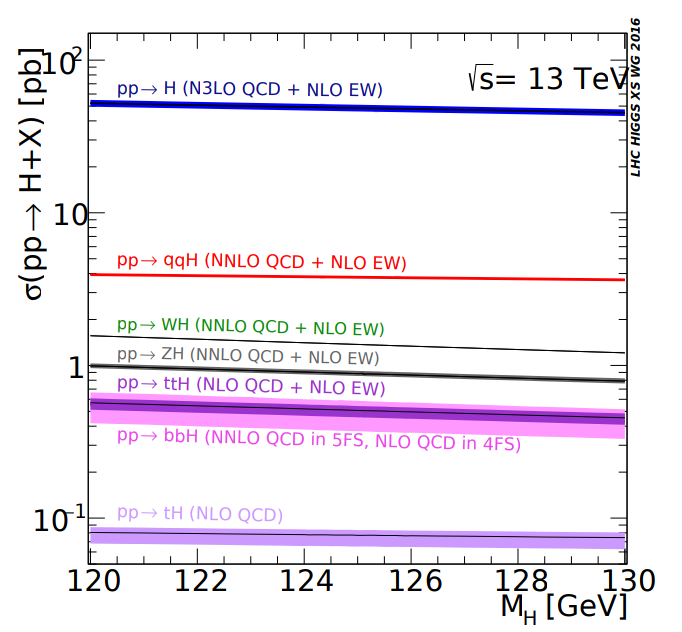
\includegraphics[width=0.5\textwidth]{figures/pheno/higgsXsec.png}
\caption{The cross sections of various higgs production mechanisms shown as a function of Higgs mass. {\color{red} address different names in plot} \cite{higgsCross}}
\label{fig:higgsCrossSection}
\end{figure}

The total production cross-section for Higgs bosons at the LHC is 54.7~pb at N3LO precision \cite{higgsCross}.
Higgs bosons are produced through several distinct mechanisms at the LHC.
These are distinguished by both their initial states and the topology of their final states.
The leading production, responsible for 89\% of all Higgs, is through gluon-gluon fusion (ggF).
Although there is no direct coupling between gluons and the Higgs, the interaction is mediated by a heavy quark loop.
The next leading production mechanism is vector boson fusion (VBF), with roughly 9\% of the cross-section as ggF.
In this process, the Higgs is produced through a ``collision'' of either \W or \Z bosons.
The final state includes the Higgs, along with two quarks that rapidly patronize to form jets.
The presence of two jets in the final state help distinguish VBF events from background processes and ameliorates the challenge of its low cross-section.
The weakest production mechanisms are ttH and bbH, where the Higgs is produced in conjunction with a top or bottom quark pair.

The production mechanisms with the third-largest cross-section are collectively called ``Higgs produced in association with a vector boson'', or VH.
These are the primary focus for the \hmm search presented in this thesis.
There are several ``sub-mechanisms'' that contribute to VH.
Of these, the one with the largest cross-section is the s-channel production with initial state quarks whimsically called \emph{Higgsstrahlung} in analogy to Bremsstrahlung radiation.
When the mediator boson is a \W, then Higgsstrahlung is responsible for the leading order WH production mechanism.
As a result of the corresponding parton luminosities, the cross-section of WH depends on the sign of the mediating $W$ boson: the production positively charged \Wp benefits from the enhanced PDF of valance $u$-quarks seen in Figure \ref{fig:partonLumi}. \check
The cross section for WH is given in Equation \ref{eqn:whxs}.

\begin{equation}\begin{split}\label{eqn:whxs}
\sigma(q_i\qbar_j\to WH)=\frac{\pi\alpha^2 |V_{ij}|^2}{36 \sin^4\theta_W} \frac{2k}{\sqrts} \frac{k^2+3m^2_W}{(s-m^2_W)^2}
\end{split}\end{equation} 
Here $V_{ij}$ are the CKM matrix elements, $k$ is the center of mass momentum of the Higgs, and $\theta_W$ is the Weinberg angle defined in Section \ref{sec:ewTheory}.

When the mediator boson is a \Z, then Higgsstrahlung is the leading production mechanism for ZH as well.
The cross section for ZH in $pp$ collisions is given in Equation \ref{eqn:zhxs}.
\begin{equation}\begin{split}\label{eqn:zhxs}
\sigma(f\overline{f}\to ZH)=\frac{\pi\alpha^2 \ell_f^2r_f^2}{48N_c\sin^4\theta_W\cos^4\theta_W} \frac{2k}{\sqrts} \frac{k^2+3m^2_Z}{(s-m^2_Z)^2}
\end{split}\end{equation} 
Here, $r\equiv-2Qx_W$, $\ell\equiv2(T_3-Qx_W$,
$T_3$ is the third component of weak isospin for the left-handed $f$, $Q$ is its electric charge, and $x_W\equiv\sin^2\theta_W$.
While Equation \ref{eqn:zhxs} describes the $q\qbar\to ZH$ cross-section, it is also applicable to $\ell^+\ell^-$ collisions that might take place in future lepton colliders.
This makes this process of particular interest for precision measurements of Higgs properties.

Unlike with WH, the sub-leading mechanisms are not negligible for ZH.
These consist of interactions with two initial state gluons where the Higgs is produced via a heavy quark loop.
There are two diagrams to consider: a ``box'' diagram and a ``triangle'' diagram.
Together, these represent $\approx10\%$ of the total ZH cross-section.

\begin{table}[htp]
\begin{center}
{\footnotesize
\begin{tabular}{l | l | l l l}
\toprule
Production & Cross section [pb] & Uncertainty (theory) [\%] & Uncertainty (PDF/$\alpha_s$) [\%] \\
\midrule
Gluon-gluon fusion (ggF)  & 48.58       & +4.56, -6.27 & $\pm3.20$  \\
Vector boson fusion (VBF) &  4.28       & +0.5, -0.3 & $\pm2.1$  \\
Associated W (WH)         & 1.513       & +0.4, -0.7 & $\pm1.8$  \\
$\hookrightarrow$  $\Wp\to\ell^+\nu$    &$\hookrightarrow$ 0.10363 &$\hookrightarrow$ +0.3, -0.8 &$\hookrightarrow$ $\pm1.8$  \\
$\hookrightarrow$  $\Wm\to\ell^-\nu$    &$\hookrightarrow$ 0.6649  &$\hookrightarrow$ +0.5, -0.6 &$\hookrightarrow$ $\pm1.9$  \\
Associated Z (ZH)         & 0.9861      & +3.8, -3.3 & $\pm1.6$  \\
$\hookrightarrow$  $Z\to\ell^+\ell^-$   &$\hookrightarrow$ 0.03327 &$\hookrightarrow$ +3.8, -3.3 &$\hookrightarrow$ $\pm1.6$  \\
ttH                       &  0.6137     & +6.0, -9.2 & $\pm3.5$  \\
\bottomrule
\end{tabular}
}
\caption{Vector boson leptonic decays include $\tau$. Higgs mass at 125 GeV.\cite{higgsCross}}
\label{tab:higgsCrossSec}
\end{center}
\end{table}

The diagrams for VH processes, along with the other leading production mechanisms, are shown in Table \ref{tab:higgsProdDiagrams}.
The cross-sections and the associated theoretical uncertainties, are given in Table \ref{tab:higgsCrossSec}.
As mentioned earlier, these cross sections depend on the Higgs mass. The Numbers in Table \ref{tab:higgsCrossSec} are calculated with \mh=125~GeV, and the functional dependence is shown in Figure \ref{fig:higgsCrossSection}.

\begin{table}[p!]
\begin{center}
{\footnotesize
\begin{tabular}{C{0.3\textwidth} C{0.5\textwidth}}
\toprule
Higgs Production & Diagram \\
\midrule
\centered{Gluon-gluon fusion}  &
\centered{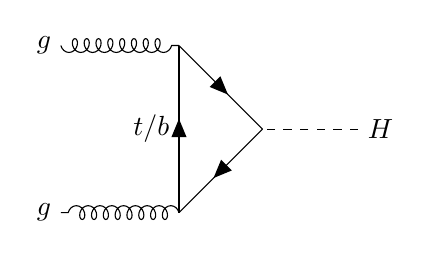
\begin{tikzpicture}
\begin{feynman}
    \vertex (h){\(H\)};
    \vertex [left=of h] (v);
    \vertex [above left=of v] (p1);
    \vertex [below left=of v] (p2);
    \vertex [left=of p1] (g1){\(g\)};
    \vertex [left=of p2] (g2){\(g\)};
    \diagram* {
    (h)[particle=\(H\)] --[scalar] (v),
    (g1)[particle=\(g\)] --[gluon] (p1) --[fermion] (v),
    (v)  --[fermion] (p2) --[gluon] (g2)[particle=\(g\)],
    (p2) --[fermion,edge label=\(t/b\)] (p1),
    };
\end{feynman}
\end{tikzpicture}} \\ [1em]
\centered{Vector boson fusion}  &
\centered{\begin{tikzpicture}
\begin{feynman}
    \vertex (h){\(H\)};
    \vertex [left=of h] (p2);
    \vertex [above=of p2] (p1);
    \vertex [below=of p2] (p3);
    \vertex [left=of p3] (qbi){\(q'\)};
    \vertex [right=of p1] (qai){\(q\)};;
    \vertex [right=of p3] (qbo){\(\qbar'\)};;
    \vertex [left=of p1] (qao){\(\qbar\)};;
    \diagram* [small,baseline=(h.base),horizontal=p2 to h] {
    (qai) --[fermion] (p1) --[fermion] (qao),
    (qbi) --[fermion] (p3) --[fermion] (qbo),
    (p1) --[boson] (p2) --[boson] (p3),
    (p2) --[scalar] (h),
    };
\end{feynman}
\end{tikzpicture}} \\ [1em]
\centered{Higgsstrahlung ZH/WH}&
\centered{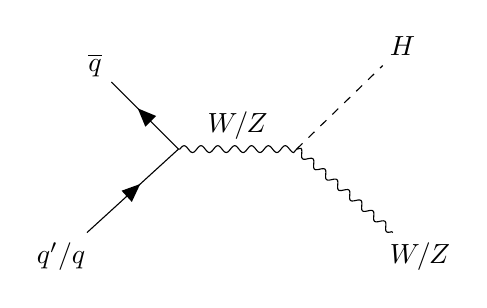
\begin{tikzpicture}
\begin{feynman}
    \vertex (qa){\(\qbar\)};
    \vertex [below right=of qa] (p1);
    \vertex [below left=of p1] (qb){\(q'/q\)};
    \vertex [right=of p1] (p2);
    \vertex [above right=of p2] (h){\(H\)};
    \vertex [below right=of p2] (v){\(W/Z\)};
    \diagram* {
    (qb) --[fermion] (p1) --[fermion] (qa),
    (p1) --[boson,edge label=\(W/Z\)] (p2),
    (v) --[boson] (p2) --[scalar] (h),
    };
\end{feynman}
\end{tikzpicture}} \\ [1em]
\centered{Gluon originated ZH\\(box diagram)} &
\centered{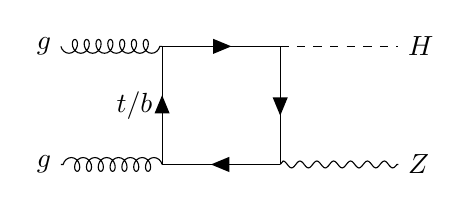
\begin{tikzpicture}
\begin{feynman}
    \vertex (g1){\(g\)};
    \vertex [right=of g1](p1);
    \vertex [right=of p1](p2);
    \vertex [right=of p2](h){\(H\)};
    \vertex [below=of g1](g2){\(g\)};
    \vertex [right=of g2](p3);
    \vertex [right=of p3](p4);
    \vertex [right=of p4](z){\(Z\)};
    \diagram* {
    (g1) --[gluon] (p1) --[fermion] (p2) --[scalar] (h),
    (z) --[boson] (p4) --[fermion] (p3) --[gluon] (g2),
    (p3) --[fermion,edge label=\(t/b\)] (p1),
    (p2) --[fermion] (p4),
    };
\end{feynman}
\end{tikzpicture}} \\ [1em]
\centered{Gluon originated ZH\\(triangle diagram)} &
\centered{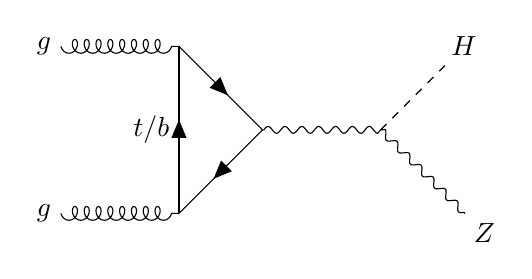
\begin{tikzpicture}
\begin{feynman}
    \vertex (h){\(H\)};
    \vertex [below left=of h](v2);
    \vertex [below right=of v2](z){\(Z\)};
    \vertex [left=of v2](v1);
    \vertex [above left=of v1](p1);
    \vertex [below left=of v1](p3);
    \vertex [left=of p1](g1){\(g\)};
    \vertex [left=of p3](g2){\(g\)};
    \diagram* {
    (g1) --[gluon] (p1) --[fermion] (v1) --[boson] (v2) --[scalar] (h),
    (z) --[boson] (v2),
    (v1) --[fermion] (p3),
    (g2) --[gluon] (p3),
    (p3) --[fermion,edge label=\(t/b\)] (p1),
    };
\end{feynman}
\end{tikzpicture}} \\ [1em]
\centered{Top associated production} &
\centered{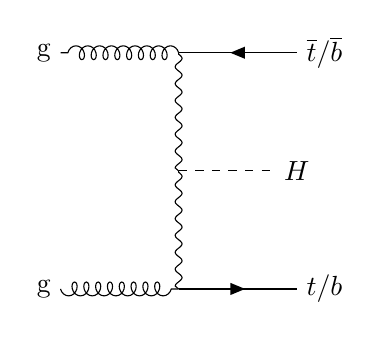
\begin{tikzpicture}
\begin{feynman}
    \vertex (h){\(H\)};
    \vertex [left=of h] (p2);
    \vertex [above=of p2] (p1);
    \vertex [below=of p2] (p3);
    \vertex [left=of p3] (qbi){g};
    \vertex [right=of p1] (qai){\(\overline{t}/\overline{b}\)};;
    \vertex [right=of p3] (qbo){\(t/b\)};;
    \vertex [left=of p1] (qao){g};;
    \diagram* [small,baseline=(h.base),horizontal=p2 to h] {
    (qai) --[fermion] (p1) --[gluon] (qao),
    (qbi) --[gluon] (p3) --[fermion] (qbo),
    (p1) --[boson] (p2) --[boson] (p3),
    (p2) --[scalar] (h),
    };
\end{feynman}
\end{tikzpicture}} \\ [1em]
\bottomrule
\end{tabular}
}
\caption{The Feynman diagrams for the leading Higgs production mechanisms at the LHC. Together, Higgsstrahlung and the two ZH diagrams comprise VH.}
\label{tab:higgsProdDiagrams}
\end{center}
\end{table}

\begin{table}[htp]
\begin{center}
\begin{tabular}{l r}
\toprule
Decay Mode & BR=$\Gamma_i/\Gamma$ [\%] \\
\midrule
$Z\to e^+e^-$           & $3.36\pm<0.01$ \\
$Z\to \mu^+\mu^-$       & $3.37\pm0.01 $ \\
$W^+\to   e^+\nu_e$     & $10.86\pm0.09$ \\
$W^+\to \mu^+\nu_\mu$   & $10.71\pm0.16$ \\
$H\to \mu^+\mu^-$       & $2.18\times10^{-2}$ (expected) \\
\bottomrule
\end{tabular}
\caption{Leptonic decay branching fractions $\Gamma_i/\Gamma$ for \W, \Z, and Higgs. \cite{pdg2018}}
\label{tab:decayCrossSec}
\end{center}
\end{table}

\begin{figure}[h!]
\captionsetup[subfigure]{position=b}
\centering
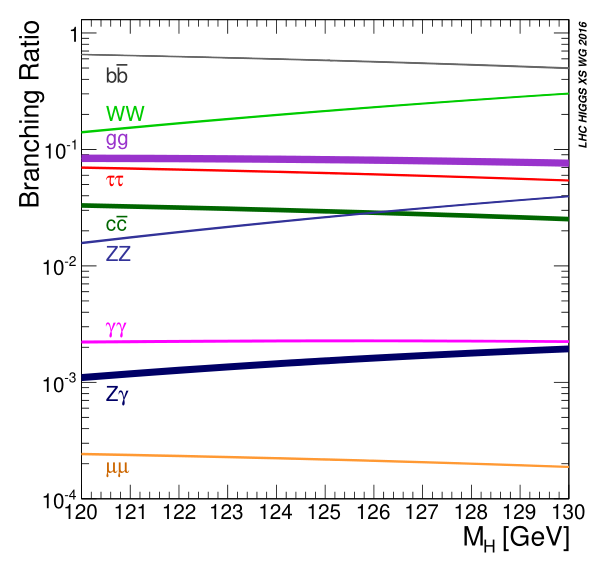
\includegraphics[width=0.5\textwidth]{figures/pheno/higgsBr.png}
\caption{}
\label{fig:higgsBr}
\end{figure}

The partial width of the Higgs boson decaying to two fermions is given by Equation \ref{eqn:higgsDecayFermions}.
\begin{equation}\begin{split}\label{eqn:higgsDecayFermions}
\Gamma(H\to ff)=\frac{G_Fm_f^2m_HN_c}{4\pi\sqrt{2}}(1-4\frac{m_f^2}{m_H^2})^{3/2}
\end{split}\end{equation} 
Here, the $N_c=1$ for leptons (and 3 for quarks) and $G_F=1.166\times10^{-5}$~GeV$^{-2}$ is the Fermi coupling constant.
The total width, $\Gamma$, is defined as the number of decays per time, per particles present.
It is the sum of all partial widths, such as the fermionic width in Equation \ref{eqn:higgsDecayFermions}.
The total width is equivalent to the reciprocal \emph{lifetime} of the particle $\tau$, which subsequently defines the particle's half-life as $\tau\ln2$.
The partial width also dictates the \emph{branching ratio} that describes the fraction of decays to a particular final state.
For \hmm decays, the branching ratio is therefore

\begin{equation}\begin{split}
    \text{BR}(\hmm)=\frac{\Gamma(\hmm)}{\Gamma}.
\end{split}\end{equation} 

This equation illuminates the central challenge when studying \hmm. 
The total width of the Higgs is expected to be $4$~MeV and has been measured as $\Gamma=3.2^{+2.8}_{-2.2}$~MeV. \cite{cmsWidth}
The quadratic dependence on the muon mass $m_f=m_\mu$ in the partial width $\Gamma(\hmm)$ leads to a small branching ratio in the case of the light muon, given in Table \ref{tab:decayCrossSec}.
The partial widths also depend on \mh. This is illustrated in Figure \ref{fig:higgsBr} for the branching ratios, including and larger than \hmm.

Experimentally, Higgs production and decay to two muons manifests itself in the dimuon invariant-mass spectrum as a resonance above a smoothly falling background.
The resonance width is determined by the total width, $ \Gamma $, by making use of the uncertainty principle in natural units.
A free particle of mass $m$ with some likelihood to decay to a lower energy state can be described by a simple time dependant wave function,
\begin{equation}\begin{split}
    \psi(t)=\psi(0)e^{-imt}e^{-\frac{\Gamma}{2}t}.
\end{split}\end{equation} 
Here, the first exponential represents a stable particle's time evolution, while the second represents the decreasing probability that the particle has not decayed.
The $\Gamma$ is the decay rate and also inverse of the exponential time constant.
The fourier transform of the wave equation describes the particle in energy space,
\begin{equation}\begin{split}
    \psi(E)=\int\psi(t)e^{iEt}dt\propto \frac{1}{(E-m)-i\Gamma/2}.
\end{split}\end{equation}
The energy dependant cross section to observe a decay is proportional to $|\psi(E)|^2$, or 
\begin{equation}\begin{split}\label{eqn:breitWigner}
    \sigma(E)\propto\frac{1}{(E-m)^2+\Gamma^2/4}.
\end{split}\end{equation} 
Equation \ref{eqn:breitWigner} gives the relativistic Breit-Wigner function, which describes resonant features in energy spectra.
The resonance width corresponds to the decay rate; therefore, particles with long lifetimes $\tau$ produce narrow resonances.

These principles determine the phenomenology of \hmm.
The Higgs boson decays with a width $\Gamma$ and the probability distribution of energies described by the Breit-Wigner function.
In \hmm decays, this energy is converted into the dimuon pair's invariant-mass and results in a narrow resonance in the dimuon invariant mass spectrum.
In practice, the energy and momentum resolutions of ATLAS are insufficient to resolve the $\approx4$~MeV width of the Breit-Wigner shape.
Instead, a distribution described approximately a Gaussian function with a width corresponding to the invariant-mass resolution is observed.

% VH leptonic
The final state \W or \Z in a VH event offers an opportunity to help identify Higgs events in the same way that the jets in VBF are useful.
This is particularly true when the \W or \Z decays leptonically since these additional leptons offer a clean signal to help remove events from background production mechanisms.
In the case of \W decays to $\ell^\pm\nu_\ell$ represent $\approx11\%$ of decays for each lepton flavor.
Equation \ref{eqn:wDecayFermions} gives the partial width for leptonic \W decays.
\begin{equation}\begin{split}\label{eqn:wDecayFermions}
    \Gamma(W\to\ell\overline{\nu})=\frac{\sqrt{2}G_Fm_W^3}{12\pi}
\end{split}\end{equation} 
The total width of the \W boson is $\Gamma=2.085\pm0.042$~GeV.
The leptonic branching fraction is smaller in the case of \Z.
The partial width for \Z decays to fermions is given in Equation \ref{eqn:zDecayFermions}.
\begin{equation}\begin{split}\label{eqn:zDecayFermions}
    \Gamma(Z\to f\fbar)=N_c\frac{\sqrt{2}G_Fm_Z^3}{6\pi}\times[(T_3-Q_f\sin^2\theta_W)^2+(Q_f\sin^2\theta_W)^2]
\end{split}\end{equation} 
The total width of the \Z boson is $\Gamma=2.495\pm0.002$~GeV, and the leptonic width is $\Gamma(\Z\to\ll)=83.984\pm0.086$~MeV per lepton flavor.
The result is a leptonic branching ratio of 3.4\% per flavor. \cite{pdg2018}
The measured values of these branching fractions are given in Table \ref{tab:decayCrossSec}.

\section{Contact Interactions and Compositeness}

Contact interactions are a phenomenological description of new physics interactions above the energy scale accessible directly in collisions.
Such interactions lead to increases in the event rate of high mass events in the dilepton invariant invariant-mass spectra. 
A broad assortment of models predicts such excesses, but particular interest models are models of composite quarks and leptons.
Even within the space of compositeness models, there is great diversity and no consensus about the plausibility of a single model. 
It is beneficial to consider the predictions in common with all compositeness models rather than a particular model.
The putative components of fermions are called \emph{preons}, and they are expected to interact through a new strong gauge interaction called \emph{metacolor}.
As is the case of the strong force, metacolor would be infrared confining and asymptotically free.
Below a characteristic energy scale \lam, the interaction binds preons together metacolor singlets observed as quarks and leptons.
While \lam remains unknown, it is clear that it exceeds the fermion masses.
The fermions remain massless relative to \lam through 't Hooft's mechanism. \cite{Eichten:1984eu}
{\color{red} The explanation is in \emph{Recent Developments in Gauge Theories} for 83 euros!}
Early theoretical limits were set by Bhabha-scattering measurements that exclude \lam below 1-2~TeV for electrons. \cite{Eichten:1984eu}
\footnote{Flavor-changing contact interactions are highly constrained through experiment, with limits on \lam excluding values up to hundreds or thousands of TeV.\cite{Eichten:1984eu}}

The particular interest of this thesis is in flavor-diagonal contact interactions.
These models allow either one or both of the fermion's chiral components (\fl and \fr) to be composite.
The presence of parity-violating in the standard model motivates the treatment of \fl and \fr as distinct species.
This leads to the general parity violating Lagrangian in Equation \ref{eqn:compLagrangian} which describes a general contact interaction.
\begin{equation}\label{eqn:compLagrangian}
\begin{array}{r@{\,}c@{}c@{\,}l@{\,}l}
\mathcal L = \frac{g^2}{2\Lambda^2}\;[ && \eta_{\mathrm{LL}}&\, (\ufl\gamma_{\mu} \fl)\,(\uflp\gamma^{\mu}\flp) \nonumber \\
& +&\eta_{\mathrm{RR}}& (\ufr\gamma_{\mu} \fr) \,(\ufrp\gamma^{\mu}\frp) \\
&+&\eta_{\mathrm{LR}}& (\ufl\gamma_{\mu} \fl) \,(\ufrp\gamma^{\mu}\frp) \\
&+&\eta_{\mathrm{RL}}& (\ufr\gamma_{\mu} \fr) \,(\uflp\gamma^{\mu}\flp)& ] \: ,\nonumber
\end{array}
\end{equation}
Here $\eta_{ij}$ for $i,j\in\{L,R\}$ are parameters dictating which species are composite: $|\eta_{LL}|=1$ describes composite left-handed fermions, while $|\eta_{LR}|=1$ indicates both \fr and \fl are composite and share common constituents.
In the form given here, a distinction is made between the initial state fermion species ($f$) and final state species ($f'$) because the present interest is in \llqq contact interactions.
This contact interaction Lagrangian describes an approximation of fermion compositeness in the $\shat\llt\lam$ regime.

\begin{figure}[h!]
\captionsetup[subfigure]{position=b}
\centering
\subfloat[][]{{
\feynmandiagram [medium,baseline=(v.base),horizontal=v to b] {
i1 [particle=\(q\)] -- [fermion] v -- [fermion] i2 [particle=\(\qbar\)],
v -- [photon, edge label=\(\gamma^*/Z\)] b,
f1 [particle=\(\ell^{+}\)] -- [fermion] b -- [fermion] f2 [particle=\(\ell^{-}\)],
};
}}
\subfloat[][]{{
\feynmandiagram [medium,baseline=(v.base),horizontal=a to c] {
a[particle=\(q\)] --[fermion] v[blob,label=\(\lam\)] --[fermion] b[particle=\(\qbar\)],
c[particle=\(\ell^{+}\)] --[fermion] v --[fermion] d[particle=\(\ell^{-}\)],
};
}}
\caption{Feynman diagrams representing (a) Drell-Yan, which dominates the standard model contribution to high invariant-mass dilepton production, and (b) a contact interaction of energy scale \lam corresponding to one of the composite models described in Equation \ref{eqn:compLagrangian}.}
\label{fig:ciPheno}
\end{figure}

Contact interactions necessarily modify cross-sections of fermion elastic scattering, such as the $q\qbar$ collisions at the LHC.
In the SM, the gauge coupling $\alpha_f$ controls high-mass processes through Drell-Yan production.
In their seminal work of 1983, Eichten, Lane, and Peskin showed that if $\alpha_f\llt1$, then the Lagrangian in Equation \ref{eqn:compLagrangian} produces interference of the order $\shat/\alpha_f\lam^2$ with the standard model processes. \cite{eichten}
The diagrams for the dominant standard model process and a generic contact interaction are shown in Figure \ref{fig:ciPheno}.
The blob in the diagram for the contact interaction emphasizes the generality of Equation \ref{eqn:compLagrangian}. A particular physics model may replace this blob with, for example, an s-channel diagram mediated by the bound state of two prions.
Two possible diagrams to replace the blob are given, for illustrative purpose, in Figure \ref{fig:ciBlobs}.

Since these interactions depend on $q\qbar$ initial states, the relevant parton luminosities that determine the event rates are those of $u\ubar$ and $d\dbar$.
Unfortunately, as illustrated in Figure \ref{fig:partDistFunc}, proton PDFs for $\ubar$ and $\dbar$ are relatively small since these are produced as virtual sea quarks.
This suppresses the production of $q\qbar$ initial states, and consequently, of this type of contact interaction.
If the LHC had been designed to use $p\pbar$ collisions of equal intensity, it would greatly enhance the $q\qbar$ luminosities.

\begin{figure}[h!]
\captionsetup[subfigure]{position=b}
\centering
\subfloat[][]{{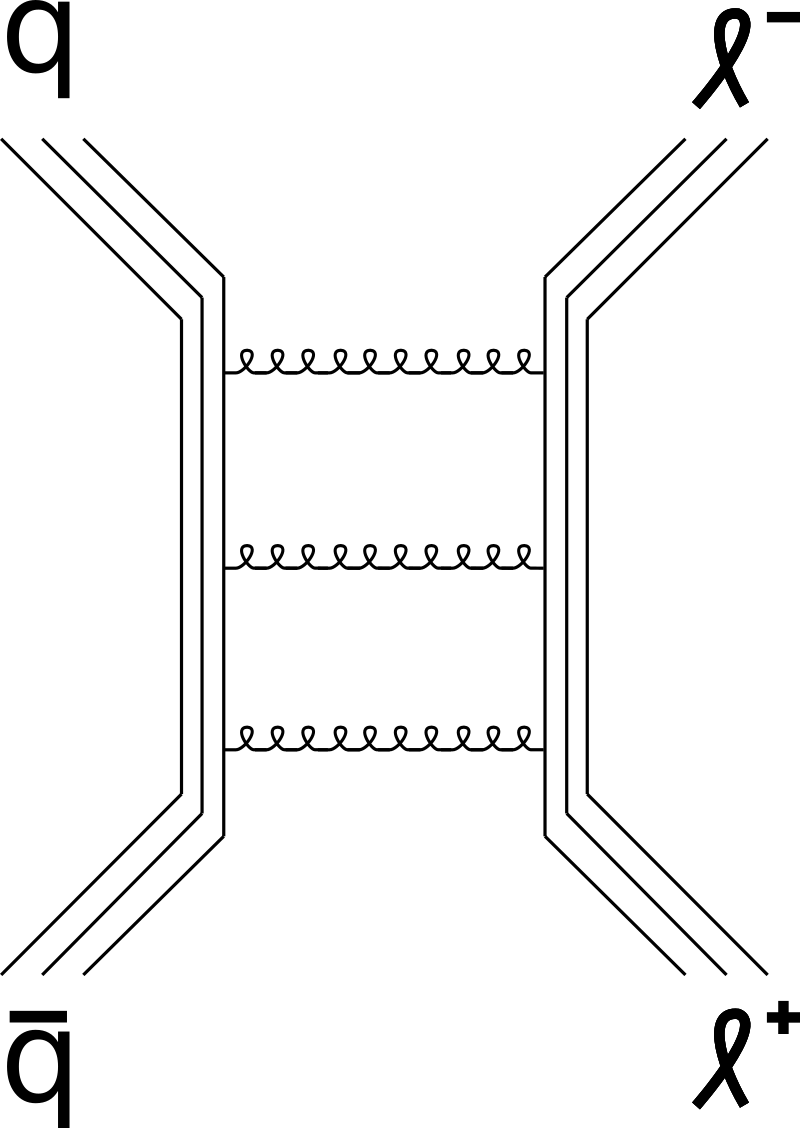
\includegraphics[height=0.20\textheight]{figures/pheno/ciGluon.png}}}
\hspace{0.15\textwidth}%
\subfloat[][]{{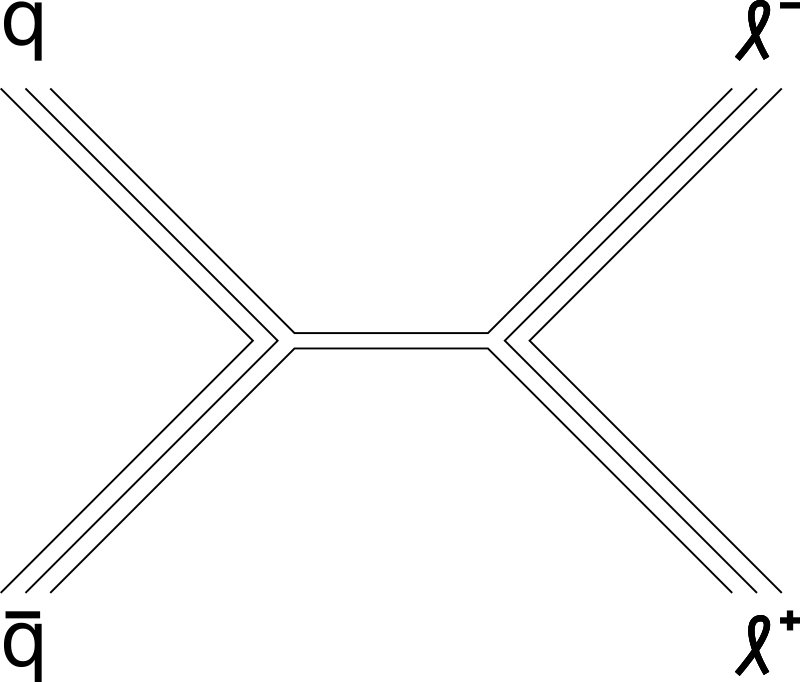
\includegraphics[height=0.20\textheight]{figures/pheno/ciSchan.png}}}
\caption{Feynman diagrams for two possible high-energy processes that may result from fermion compositeness. The solid lines represent the preons composing the fermions. In subfigure (a), an interaction mediated by the bound state of two prions, which is only possible when the leptons and quarks share common constituents. In subfigure (b), an interaction between quarks and leptons mediated by ``metacolor gluon'' exchange, represented by curly lines in analogy to SU(3) gluons.{\color{red} Find way to make better diagrams}}
\label{fig:ciBlobs}
\end{figure}

%%% Specific ll-qq CI $$$
This thesis focuses on \llqq contact interactions, a subset of those described by Equation \ref{eqn:compLagrangian}.
Such models replace the unprimed $f$ with quarks, and the primed $f'$ with leptons.
This interaction is possible if the quarks and leptons share common constituents, in which case interactions mediated by the constituents are possible, as shown in Figure \ref{fig:ciBlobs} (a).
This interaction is also possible if the fermions do not share common constituents, as shown in Figure \ref{fig:ciBlobs} (b).

The Drell-Yan differential cross-section is modified in the case of left-left compositeness, $\eta_{LL}=\pm1$ and $\eta_{LR}=\eta_{RL}=\eta_{RR}=0$.

\begin{flalign}\label{eqn:}
\frac{d\hat{\sigma}}{d\that}(q_i\qbar_i\to\ll) =& \frac{\pi\alpha^2}{\shat^2}\left[A_i(\shat)\left(frac{\uhat}{\shat}\right)^2+B_i(\shat)\left(frac{\that}{\shat}\right)^2\right] \notag\\
\end{flalign} 
Here, the coefficients are defined as functions of \shat.
\begin{flalign}\label{eqn:}
A_i(\shat) =& \left[Q_i-\frac{L_iL_l}{4x_W(1-x_w)}\frac{\shat}{\shat-M_Z^2+iM_Z\Gamma_Z}-\frac{\eta_{LL}\shat}{\alpha\lam^2}\right]^2 + \notag\\
            & \left[Q_i-\frac{R_iR_l}{4x_W(1-x_w)}\frac{\shat}{\shat-M_Z^2+iM_Z\Gamma_Z}\right]^2  \notag\\
B_i(\shat) =& \left[Q_i-\frac{R_iL_l}{4x_W(1-x_w)}\frac{\shat}{\shat-M_Z^2+iM_Z\Gamma_Z}\right]^2 + \notag\\
            & \left[Q_i-\frac{L_iR_l}{4x_W(1-x_w)}\frac{\shat}{\shat-M_Z^2+iM_Z\Gamma_Z}\right]^2  \notag\\
\end{flalign}
In these equations, $i,j\in\{u,d\}$ stand for quark flavors.
As was defined when discussing Higgs production in Section \ref{sec:phenoHiggs}, $L_i=T_3-2Q_ix_W$, $R_i=-2Q_ix_W$, and $x_W=\sin^2\theta_W$. {\color{red} coordinate notation}
$Q_i$ is the electric charge of the corresponding quark flavor. \cite{Eichten:1984eu} % supercollider

Despite their verbosity, these equations readily illuminate the phenomenology relevant to the contact interaction search.
First, when setting $\eta_{LL}=0$, the standard model Drell-Yan production is recovered.
Expanding the first power term in $A_i(\shat)$ yields a \emph{direct} term that contributes to the total cross-section and scales as $\lam^{-4}$.
Removing the \lam defines the contact interaction form factor $F_C$,
\begin{equation}\begin{split}
    % \Delta\left[\frac{d\hat{\sigma}}{d\that}\right] = \frac{\pi\alpha^2}{\shat^2}\left[\frac{\shat}{\alpha^2}\left(\frac{\uhat}{\shat}\right)^2 \right] /\lam^4
    F_C(\shat) \equiv \frac{\pi\uhat^2}{\shat^2}.
\end{split}\end{equation} 
{\color{red} Check d\that vs d\mll}
Since $F_C$ is strictly positive, it enhances the total \qqll cross section regardless of the sign of $\eta_{LL}$.
The cross-terms in the expansion dictate the interference of the contact interaction with Drell-Yan.
Again removing the \lam factor defines the interference form factor $F_I$,
\begin{equation}\begin{split}
    F_I(\shat) \equiv -2\eta_{LL}\left[Q_i-\frac{L_iL_l}{4x_W(1-x_w)}\frac{\shat}{\shat-M_Z^2+iM_Z\Gamma_Z}\right]\frac{\pi\alpha\uhat^2}{\shat^3}.
\end{split}\end{equation} 
The sign of $F_I$ depends on the sign of $\eta_{LL}$.
For $\eta_{LL}=-1$, $F_I$ contributes constructively to the total cross-section, while for $\eta_{LL}=+1$ it leads to destructive interference that reduces the overall cross-section.

Together, $F_I$ and $F_C$ describe the effect of contact interactions as functions of collision energy, without referring to the particular manifestation of fermion compositeness.
The functional dependence on \shat leads to the expression of the interference form factor $F_I$ at relatively low energies than the direct form factor $F_C$.
Experimentally, this results in interference effects altering dilepton spectra at lower invariant-mass and direct production always enhancing the spectra in the high mass tail.
These effects are broad in the invariant-mass spectra instead of the narrow resonance expected from \hmm production.
The modification to the total cross section has the form,
\begin{equation}\label{eqn:cixsPheno}
\frac{\text{d}\sigma}{\text{d}m_{\ell\ell}} = \frac{\text{d}\sigma_\textrm{DY}}{\text{d}m_{\ell\ell}} - \eta_{ij}\frac{F_\textrm{I}}{\Lambda^2} + \frac{F_\textrm{C}}{\Lambda^4}.
\end{equation}

Although various compositeness models predict variations on these results, there are two points to consider.
First, the functional dependence on the energy \shat is common for all contact interactions. \cite{Eichten:1984eu}.
Second, the modification to the effect on the total cross-section is of the same magnitude regardless of the form of compositeness.
Combined, these make the described formalism an attractive framework to study compositeness without reference to the particular model.


% \cite{acosta} % LHC prospect



% \input{sections/phenomenology-objects}

\chapter{Datasets}

\section{Simulation}

The list of simulated datasets is provided in Table \ref{tab:simulatedDatasets}.

\begin{table}[htp]
\begin{center}
\resizebox{\textwidth}{!}{
\begin{tabular}{l l l l l l l l}
\toprule
Process           & QCD      & EW       & ME Generator           & PS and Hadronization \\
Drell-Yan         & NNLO     & NLO      & \powheg, CT10          & \pythia+\evtgen, CTEQ6L1   \\
Drell-Yan         & LO       &          & \powheg, NDPDF23LO     & \pythia+\evtgen, NNPDF23LO \\
$t\overline{t}$   & NLO      &          & \powheg, NDPDF3.0NLO   & \pythia+\evtgen, NNPDF23LO \\
Single top        & NLO      &          & \powheg, NDPDF3.0NLO   & \pythia+\evtgen, NNPDF23LO \\
Diboson           &          &          & \sherpa, CT10          & \sherpa, CT10              \\
\midrule
Drell-Yan         & NLO      & NLO      & \sherpa, NNPDF30NNLO   &                            \\
$t\overline{t}$   & NNLO     &          & \powheg, NNPDF3.0LO    & \pythia+\evtgen            \\
Single top        & NNLO     &          & \powheg, NNPDF3.0LO    & \pythia+\evtgen            \\
Diboson           & NLO      &          & \sherpa, NNPDF3.0LO    & \pythia+\evtgen            \\
ggH               & NNLO     &          & \powheg, PDF4LHC15     & \pythia+\evtgen            \\
VBF               & NLO      &          & \powheg, NNPDF3.0      & \pythia+\evtgen            \\
$qq/qg\to WH$     & NLO      &          & \powheg, NNPDF3.0      & \pythia+\evtgen            \\
$qq/qg\to ZH$     & NLO      &          & \powheg, NNPDF3.0      & \pythia+\evtgen            \\
$gg   \to ZH$     & LO       & LO       & \powheg, NNPDF3.0      & \pythia+\evtgen            \\
ttH               & NLO      & NLO      & \madgraph, NNPDF3.0LO  & \pythia+\evtgen            \\
\bottomrule
\end{tabular}
}
\caption{Samples in the top are used in the \nr analysis, while samples in the bottom are used for the \hmm search. {\color{red} Missing LO/NLO for some samples, afterburner details}}
\label{tab:simulatedDatasets}
\end{center}
\end{table}


\section{Physics Data}\label{sec:physData}

Both the \hmm search and the non-resonant search use the full dataset collected by ATLAS during the LHC's Run 2 period.
Only events recorded during good operation of the detector are used.
The Good Run Lists (GRL) identify the data taking periods during which the data used for analysis was collected.
Table \ref{tab:GRLs} summarizes the datasets and luminosities for each year.

\begin{table}[h]
    \begin{center}\small
        \begin{tabular}{ccl}
            \toprule
            Year & Luminosity ($\mathrm{pb}^{-1}$) & Good Runs List \\
            \midrule
            2015 & 3219.56 & \texttt{data15\_13TeV/20170619/physics\_25ns\_21.0.19.xml}\\[1ex]
            2016 & 32995.4 & \texttt{data16\_13TeV/20180129/physics\_25ns\_21.0.19.xml}\\[1ex]
            2017 & 44307.4 & \texttt{data17\_13TeV/20180619/physics\_25ns\_Triggerno17e33prim.xml}\\[1ex]
            2018 & 58450.1 & \texttt{data18\_13TeV/20190318/physics\_25ns\_Triggerno17e33prim.xml}\\[1ex]
            \bottomrule
        \end{tabular}
        \caption{Good Runs List.}
        \label{tab:GRLs}
    \end{center}
\end{table}


% % % % \chapter{Statistics}

\section{Definitions}
\subsection{Likelihood}
\subsection{CLs}
\subsection{Significance}
\subsection{Limits}

\section{Approaches to Statistics}
\subsection{Frequentist Methods}
\subsection{Bayesian Methods}
\subsection{Hybrid Methods}

% results
\section{Analyzing Data}
\subsection{Fitting Procedures}
\subsection{Measuring Significance}
\subsection{Setting Limits}

\chapter{Higgs Decay to Two Muons}

\section{Motivation}
\section{Event Selection}
\section{Signal Modeling}
\section{Background Modeling}
\section{Uncertainties}
\section{Statistical Analysis}
\section{Results}


\chapter{Non-resonant Search for Contact Interactions}\label{sec:ci}

\input{sections/contactInteractions-intro}
\section{Motivation}\label{sec:ciMotivation}

The presence of a new interaction can be detected at an energy much lower than that required to produce direct evidence of the existence of a new gauge boson. The charged weak interaction responsible for nuclear $\beta$ decay provides such an example. A non-renormalizable description of this process was successfully formulated by Fermi in the form of a four-fermion contact interaction~\cite{Fermi:1934hr}. A contact interaction can also accommodate deviations from the SM in proton--proton scattering due to quark and lepton compositeness, where a characteristic energy scale $\Lambda$ corresponds to the binding energy between fermion constituents. A new interaction or compositeness in the process $q\overline{q} \to \ell^+\ell^-$ can be described by the following four-fermion contact interaction Lagrangian~\cite{eichten, Eichten:1984eu},

\begin{equation}\label{eqn:ciLagrangian}
\begin{array}{r@{\,}c@{}c@{\,}l@{\,}l}
\mathcal L = \frac{g^2}{\Lambda^2}\;[ && \eta_{\mathrm{LL}}&\, (\overline q_{\mathrm L}\gamma_{\mu} q_{\mathrm L})\,(\overline\ell_{\mathrm L}\gamma^{\mu}\ell_{\mathrm L}) \nonumber \\
& +&\eta_{\mathrm{RR}}& (\overline q_{\mathrm R}\gamma_{\mu} q_{\mathrm R}) \,(\overline\ell_{\mathrm R}\gamma^{\mu}\ell_{\mathrm R}) \\
&+&\eta_{\mathrm{LR}}& (\overline q_{\mathrm L}\gamma_{\mu} q_{\mathrm L}) \,(\overline\ell_{\mathrm R}\gamma^{\mu}\ell_{\mathrm R}) \\
&+&\eta_{\mathrm{RL}}& (\overline q_{\mathrm R}\gamma_{\mu} q_{\mathrm R}) \,(\overline\ell_{\mathrm L}\gamma^{\mu}\ell_{\mathrm L})& ] \: ,\nonumber
\end{array}
\end{equation}

\noindent where $g$ is a coupling constant chosen by convention to satisfy $g^2/4\pi = 1$, $\Lambda$ is the contact interaction scale, and $q_{\mathrm L,R}$ and $\ell_{\mathrm L,R}$ are left-handed and right-handed quark and lepton fields, respectively. The parameters $\eta_{ij}$, where $i$ and $j$ are L or R (left or right),  define the chiral structure of the new interaction. Different chiral structures are investigated here, with the left-right model obtained by setting $\eta_{\mathrm{LR}} = \pm 1$ and $\eta_{\mathrm{RL}} = \eta_{\mathrm{LL}} = \eta_{\mathrm{RR}} = 0$. Likewise, the left-left, right-left, and right-right models are obtained by setting the corresponding parameters to $\pm 1$, and the others to zero. The sign of $\eta_{ij}$ determines whether the interference is constructive ($\eta_{ij} = -1$) or destructive ($\eta_{ij} = +1$). 

In the context of CI searches with dilepton final states at the LHC, the terms in Equation \ref{eqn:CIlagrangian} take the form of $\eta_{ij}\left(\bar{q}_i\gamma_{\mu}q_i\right)\left(\bar{\ell}_j\gamma^{\mu}\ell_j\right)$, where $q_i$ and $\ell_j$ are the quark and lepton fields, respectively.
The differential cross-section for the process $q\bar{q}\rightarrow\ell^+\ell^-$, in the presence of CI, can be separated into the SM DY term plus terms involving the CI.
This separation is given in Equation \ref{eqn:cixs}.
\begin{equation}
\frac{\text{d}\sigma}{\text{d}m_{\ell\ell}} = \frac{\text{d}\sigma_\textrm{DY}}{\text{d}m_{\ell\ell}} - \eta_{ij}\frac{F_\textrm{I}}{\Lambda^2} + \frac{F_\textrm{C}}{\Lambda^4},
\label{eqn:cixs}
\end{equation}
Here, the first term accounts for the DY process, the second term corresponds to the interference between the DY and CI processes, and the third term corresponds to the pure CI contribution.
The latter two terms include $F_\textrm{I}$ and $F_\textrm{C}$, respectively, which are functions of the differential cross-section with respect to $m_{\ell\ell}$ with no dependence on $\Lambda$~\cite{Eichten:1984eu}.
The interference can be constructive or destructive and it is determined by the sign of $\eta_{ij}$.

\begin{figure}[htb]
\begin{center}
\begin{equation}\begin{split}
\left|
\feynmandiagram [medium,baseline=(v.base),horizontal=v to b] {
i1 [particle=\(q\)] -- [fermion] v -- [fermion] i2 [particle=\(\overline{q}\)],
v -- [photon, edge label=\(\gamma/Z\)] b,
f1 [particle=\(\ell^{+}\)] -- [fermion] b -- [fermion] f2 [particle=\(\ell^{-}\)],
};
+
\feynmandiagram [medium,baseline=(v.base),horizontal=a to c] {
a[particle=\(q\)] --[fermion] v[blob] --[fermion] b[particle=\(\overline{q}\)],
c[particle=\(\ell^{+}\)] --[fermion] v --[fermion] d[particle=\(\ell^{-}\)],
};
\right|^2
\end{split}\end{equation} 

\end{center}
\vspace{-.4cm}
\caption{Leading-order production mechanism for Drell-Yan with additional contact term with scale $\Lambda$ in the dilepton final state.}
\label{FeynmanCI}
\end{figure}

Previous searches for CI have been carried out in neutrino--nucleus and electron--electron scattering~\cite{Anthony:2005pm}, as well as electron--positron~\cite{Abdallah:2008ab, Schael:2006wu}, electron--proton~\cite{Aaron:2011mv}, and proton--antiproton colliders~\cite{Abulencia:2006iv,Abazov:2009ac}. Searches for CI have also been performed by the ATLAS and CMS Collaborations~\cite{Aad:2014wca, Khachatryan:2014fba}. The strongest exclusion limits for $\ell\ell q q$ CI in which all quark flavours contribute come from the previous ATLAS non-resonant dilepton analysis conducted using 36.1\fb of proton--proton ($pp$) collision data at $\sqrt{s}$ = 13~TeV~\cite{Aaboud:2016cth}. That combined analysis of the dielectron and dimuon channels set lower limits at 95\% credibility level (C.L.) on the left-left model of $\Lambda$ $=$ 40.1~TeV and $\Lambda$ $=$ 25.4~TeV, for constructive and destructive interference, respectively, given a uniform positive 1/$\Lambda^2$, shown in Figure~\ref{LOZp}.

Other ATLAS studies of note include the 2012/2014 search for contact interactions at $7/8$ TeV at ATLAS \cite{EXOT-2013-19}, \cite{EXOT-2012-17}.


\section{Data and Event Selection}\label{sec:ciEvSel}

The search for non-resonant features in the dilepton invariant-mass spectra is concerned with collisions that produce two leptons.
This section details the event selection, data, and simulation used in the analysis.
Finally, comparisons between the recorded data and simulation are provided.


\subsection{Event Selection}
During Run 2, roughly $10^{16}$ proton collisions took place in ATLAS. \check
Since many of these events are uninteresting for the purpose of a dilepton analysis, only events meeting appropriate criteria are considered.
This reduces the total number of data events considered for the analysis to {\color{red}XXX} dimuon events and {\color{red}YYY} dielectron events.

% GRL
Only events recorded during good operation of the detector are used.
The following Good Run Lists identify the data taking periods during which the data used for analysis was collected.
\begin{itemize}
	\item 2015: data15\_13TeV.periodAllYear\_DetStatus-v89-pro21-02\_Unknown\_PHYS \\ \_StandardGRL\_All\_Good\_25ns.xml
	\item 2016: data16\_13TeV.periodAllYear\_DetStatus-v89-pro21-01\_DQDefects-00-02-04 \\ \_PHYS\_StandardGRL\_All\_Good\_25ns.xml
	\item 2017: data17\_13TeV.periodAllYear\_DetStatus-v99-pro22-01\_Unknown \\ \_PHYS\_StandardGRL\_All\_Good\_25ns\_Triggerno17e33prim.xml
	\item 2018: data18\_13TeV.periodAllYear\_DetStatus-v102-pro22-04\_Unknown\_PHYS \\ \_StandardGRL\_All\_Good\_25ns\_Triggerno17e33prim.xml
\end{itemize}

% Trigger
The first requirement for an event to be considered is the trigger: events must be identified as interesting by the ATLAS trigger system in order to be recorded.
The triggers used during data collection differ from year to year. 
In the dielectron channel, the following trigger requirements are applied.
\begin{itemize}
	\item 2015: 2e12\_lhloose\_L12EM10VH
	\item 2016: 2e17\_lhvloose\_nod0
	\item 2017 and 2018: 2e24\_lhvloose\_nod0
\end{itemize}
Although events passing these triggers are expected to contain two electrons, both may not be reconstructed. 
A subsequent requirement for two electrons to be reconstruction is made in the following selection.

In the dimuon channel, the following trigger requirements are applied.
\begin{itemize}
	\item 2015: mu26\_imedium or mu50
	\item 2016, 2017 and 2018: mu26\_ivarmedium or mu50
\end{itemize}
These trigger on events with single isolated muons. 
The choice to use these, rather than a two muon trigger, was made to increase the efficiency of the trigger for dimuon events.
The requirement for an event to have two muons is made in the following selection.

% Object selection
After passing the trigger requirement, events are evaluated under selection criteria.
In events where multiple vertices are reconstructed, the vertex with the largest $\sum\pt^2$ is the \emph{primary vertex}.
Events are required to have two Inner Detector tracks associated with the primary vertex.
The first step is to define what objects are considered in each event, based on the object definitions from Section \ref{sec:physObjects}.
Many of the technical terms used here follow the definitions found in that section.

Next, certain requirements are made as to the where the objects were reconstructed in the detector. 
This defines the fiducial region in which the search is carried out.
This definition differs for electrons and muons.

Electrons are defined using the \code{MediumLLH} identification.
They are required to pass \emph{Gradient} isolation.
Additionally, they must not be from a ``bad'' calorimeter cluster (\code{BADCLUSELECTRON}), and several other requirements.
The electron energy is calibrated using \code{es2017\_R21\_v1} (\code{ESModel}).
To study electron systematics, additional loose selection for electrons is also made, called the \emph{loose selection}.
This is otherwise the same as the nominal electron selection.
The kinematic criteria for both electron selections are listed in Table \ref{tab:ciElectronSel}.

\begin{table}[!htb]
\caption{Selection criteria for electrons. Parameters $d_{0}$ and $z_{0}$ are the transverse and longitudinal displacements of the track associated with the electron, and the vertex.}
\begin{center}
    \begin{tabular}[ht]{l l}
    \toprule
    Feature & Criteria \\
    \midrule
    Pseudorapidity range & $(|\eta| < 1.37) \quad || \quad (1.52 < |\eta| < 2.47)$ \\
    Transverse momentum & p$_T$ $>$ 30~GeV \\
    Track impact parameter significance & $|d_{0}^{BL}(\sigma)|$ $<$ 5 \\
    Track $z$ displacement & $|\Delta z_{0}^{BL} \sin{\theta}| <$ 0.5~mm \\
    \bottomrule
    \end{tabular}
\end{center}
\label{tab:ciElectronSel}
\end{table}

Muons are defined using the High-$p_T$ selection working point, and must pass the \code{FCTightTrackOnly} isolation requirement.
An additional cut, the \emph{Bad Muon Veto}, is required to reject muons with large \pt uncertainty.
The remaining kinematic criteria for muons are given in Table \ref{tab:ciMuonsSel}.

\begin{table}[ht]
\caption{Selection criteria for muons. Parameters $d_{0}$ and $z_{0}$ are the transverse and longitudinal displacements of the track associated with the muon, and the vertex.}
\begin{center}
    \begin{tabular}[ht]{l l}
    \toprule
    Feature & Criteria \\
    \midrule
    Transverse momentum  & $\pt>30$ GeV\\
    Pseudorapidity range & $|\eta|<2.5$ \\
    Track impact parameter significance & $|d_{0}^{BL}(\sigma)|< 3$ \\
    Track $z$ displacement  & $|\Delta z_{0}^{BL} \sin{\theta}| < 0.5~mm$\\
    \bottomrule
    \end{tabular}
\end{center}
\label{tab:ciMuonsSel}
\end{table}

Occasionally, the interaction of a single particle with detectors results in the reconstruction of two particles.
To avoid this, and \emph{overlap removal} scheme removes particles that are suspiciously close to each other.
The criteria are listed in Table \ref{tab:ciOr}.
\begin{table}[ht]
\caption{Overlap removal}
\begin{center}
    \begin{tabular}[ht]{l l l}
    \toprule
    Reject & Against & Criteria \\
    \midrule
    Electron & Electron & Shared ID track, $\pt^1<\pt^2$ \\
    Muon     & Electron & Is calo-muon and shared ID track \\
    Electron & Muon     & Shared ID track \\
    \bottomrule
    \end{tabular}
\end{center}
\label{tab:ciOr}
\end{table}
Further rejection of muons and electrons takes place if a jet is reconstructed within an angular distance $\delta R<0.4$.

% Event selection
The requirements listed so far define a set of events to consider, and a set of objects in each event.
It remains to determine whether the event is interesting with respect to the present analysis.
In general, events containing either a two electrons or two muons are of interest.
Of the same-flavor leptons in the event, the leading and subleading \et (\pt) pair are selected in the electron (muon) channel.
In the muon channel, only pairs with opposite charged muons are considered. 
In the electron channel, the charge is ignored since bremsstrahlung emission of photons can lead the electron track to bend, leading to miss-identification of the charge.
Finally, a preliminary invariant mass cut of $\mll>130$~GeV is required.
In the case where both a dielectron and dimuon candidate meet these requirements, the dielectron is selected and the dimuon is discarded.
This choice is made due to the preferable electron \et resolution at high energy.

\subsection{Data}
The data used in this analysis was collected during the LHC's Run 2.
The recorded integrated luminosity of the collisions is $139\pm2$ \fb. \cite{ATLAS-CONF-2019-021}

The data yield rate, broken into the different runs and periods for each year, are shown in Figure ~\ref{fig:ciYields}.
These plots count events after applying the full selections.

\begin{figure}[ht!]
\captionsetup[subfigure]{position=b}
\centering
\subfloat[][]{{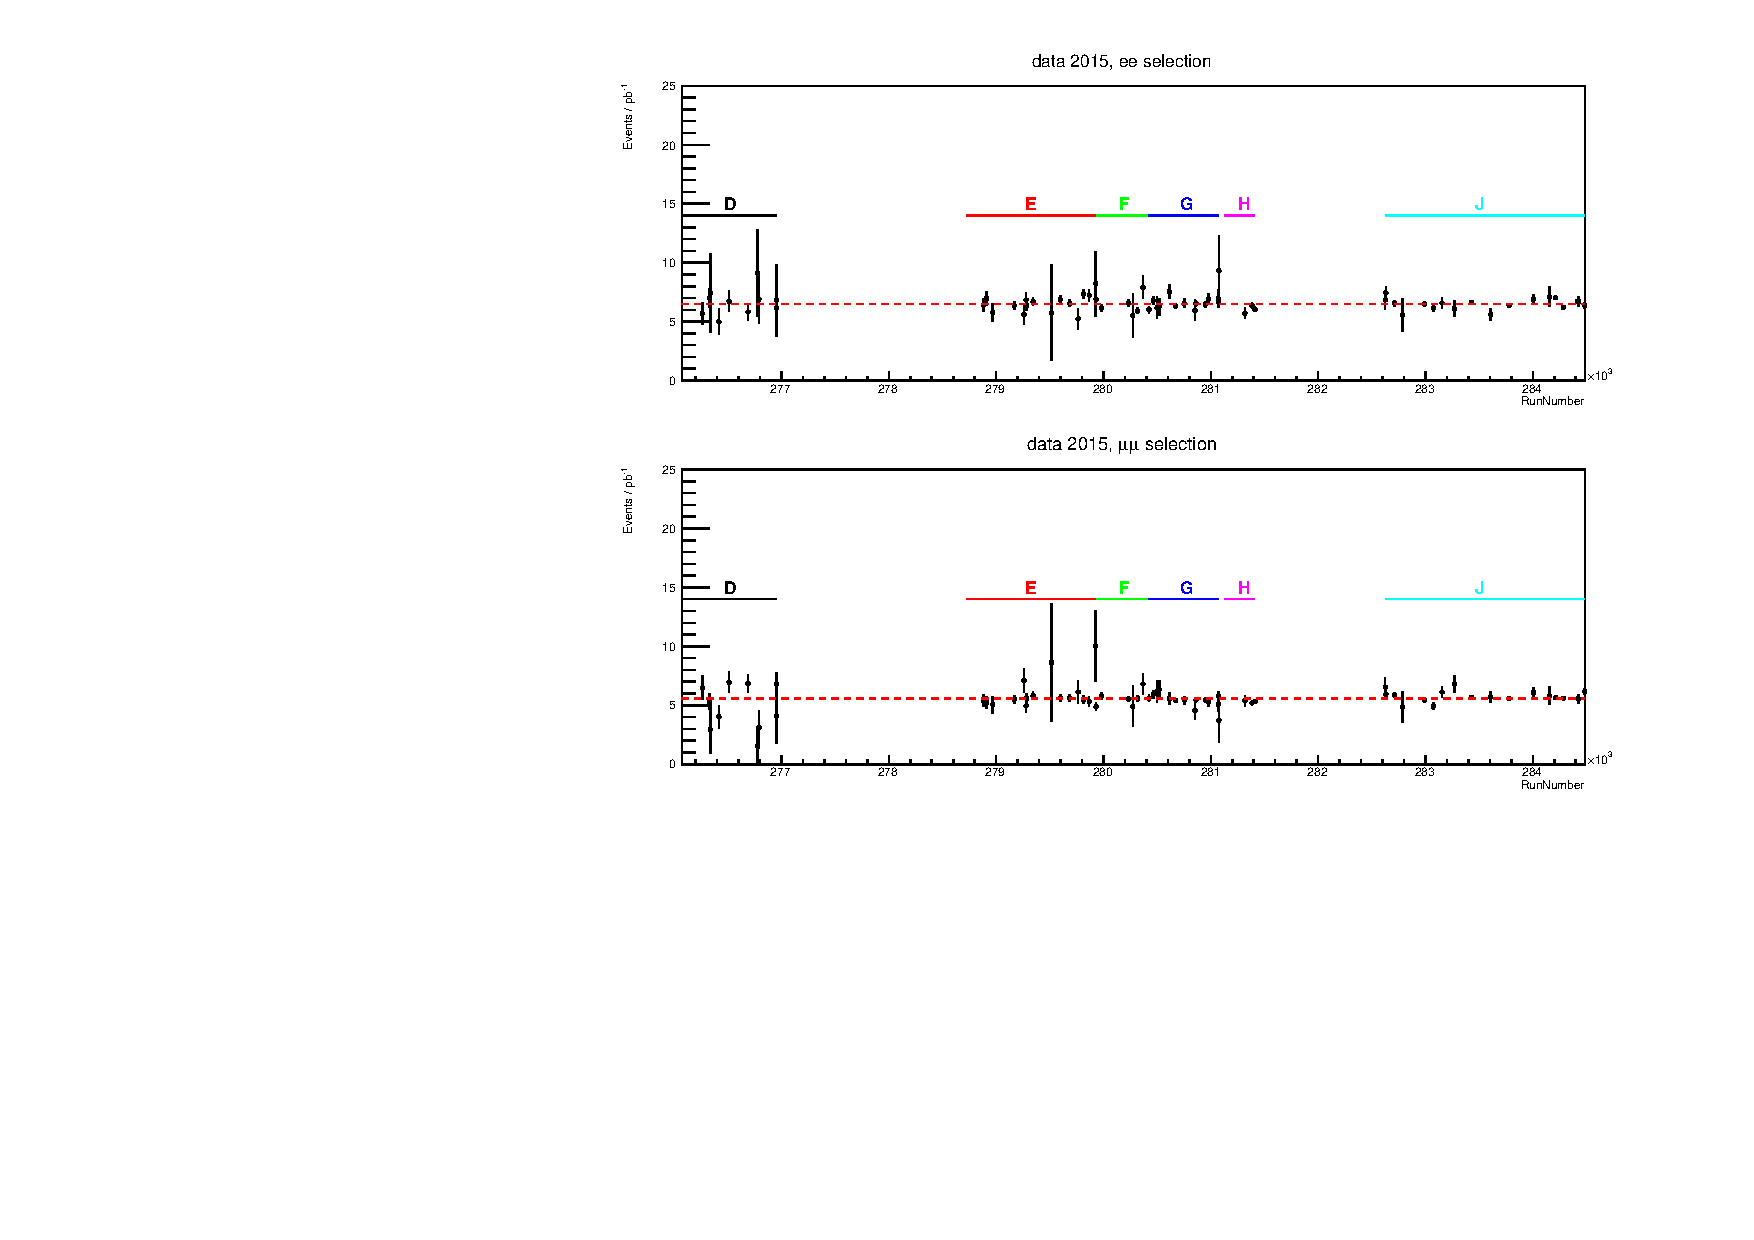
\includegraphics[width=0.48\textwidth]{figures/ci/dataMc/compare_data_yields2015.pdf}}}
\subfloat[][]{{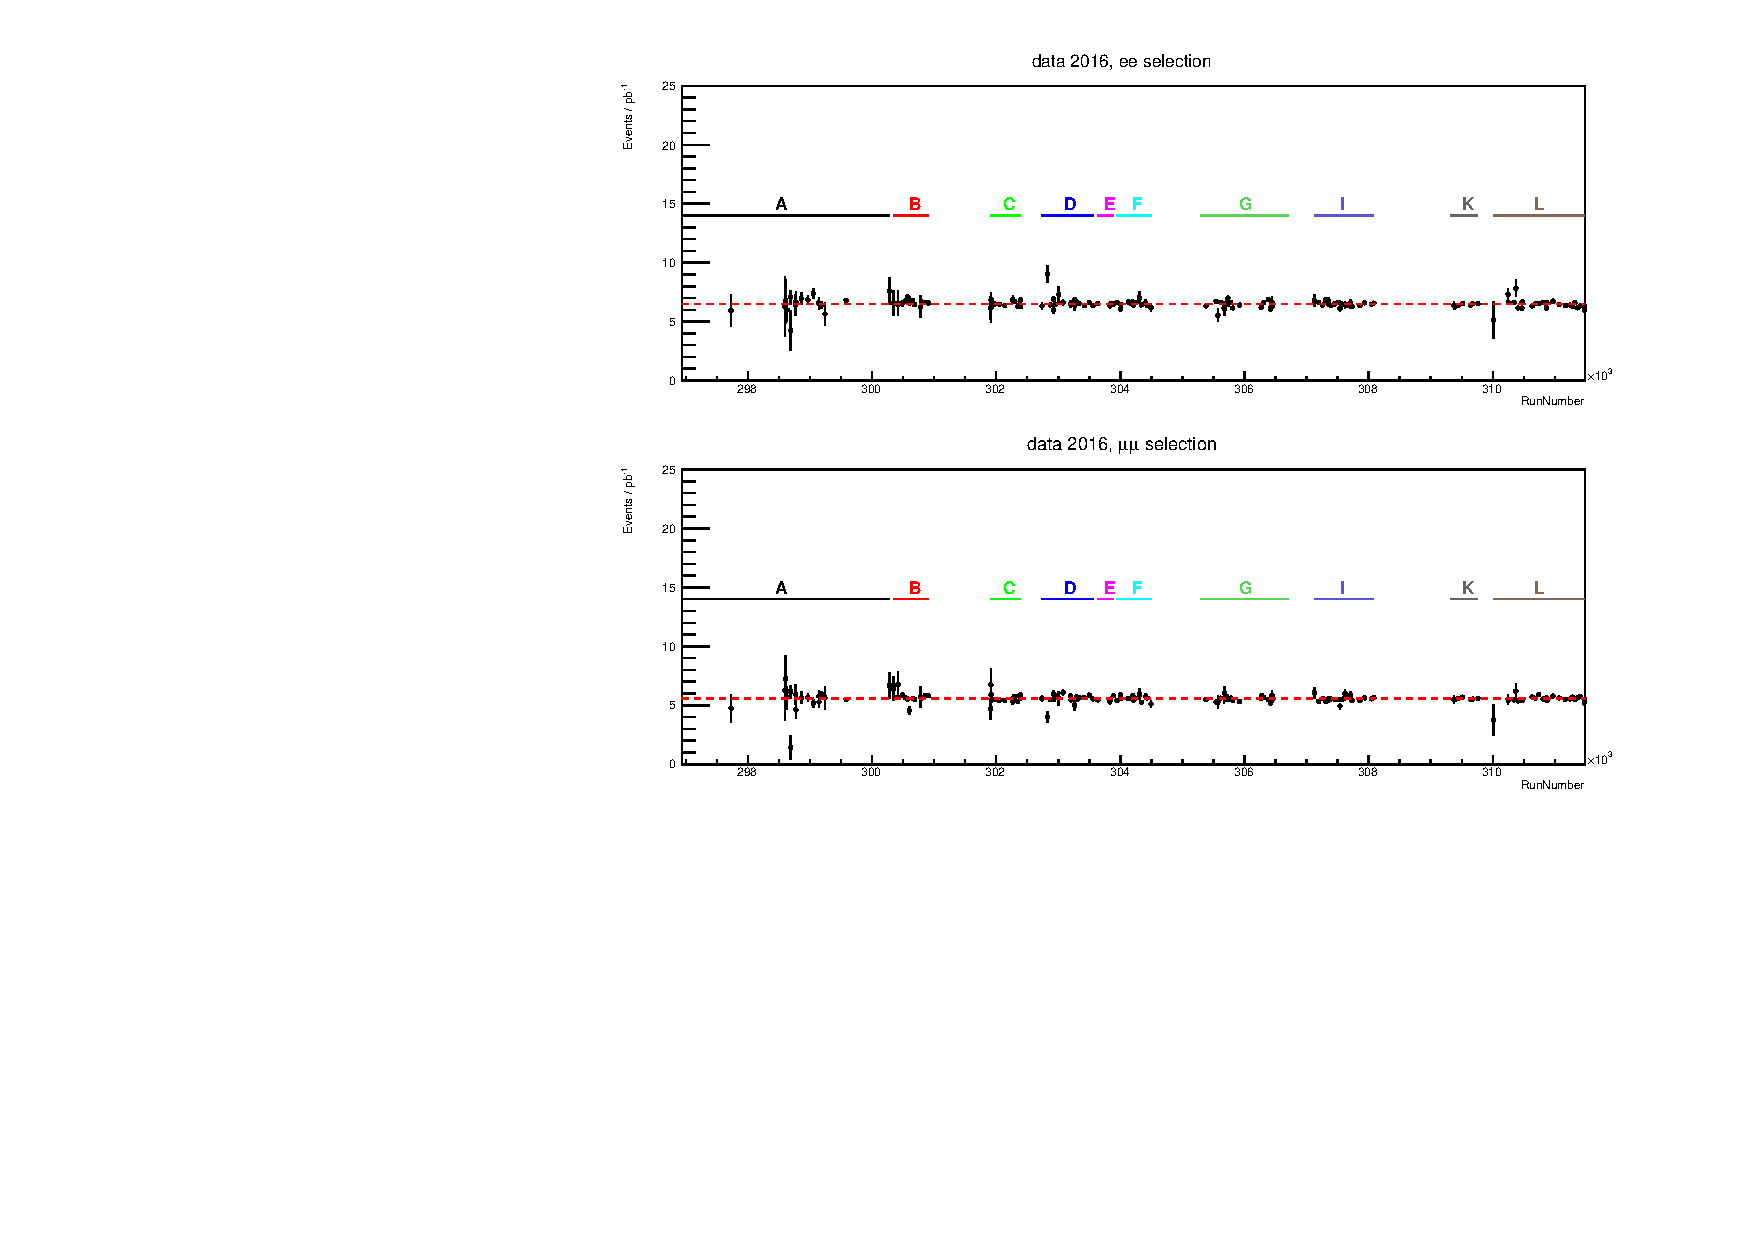
\includegraphics[width=0.48\textwidth]{figures/ci/dataMc/compare_data_yields2016.pdf}}}\\
\subfloat[][]{{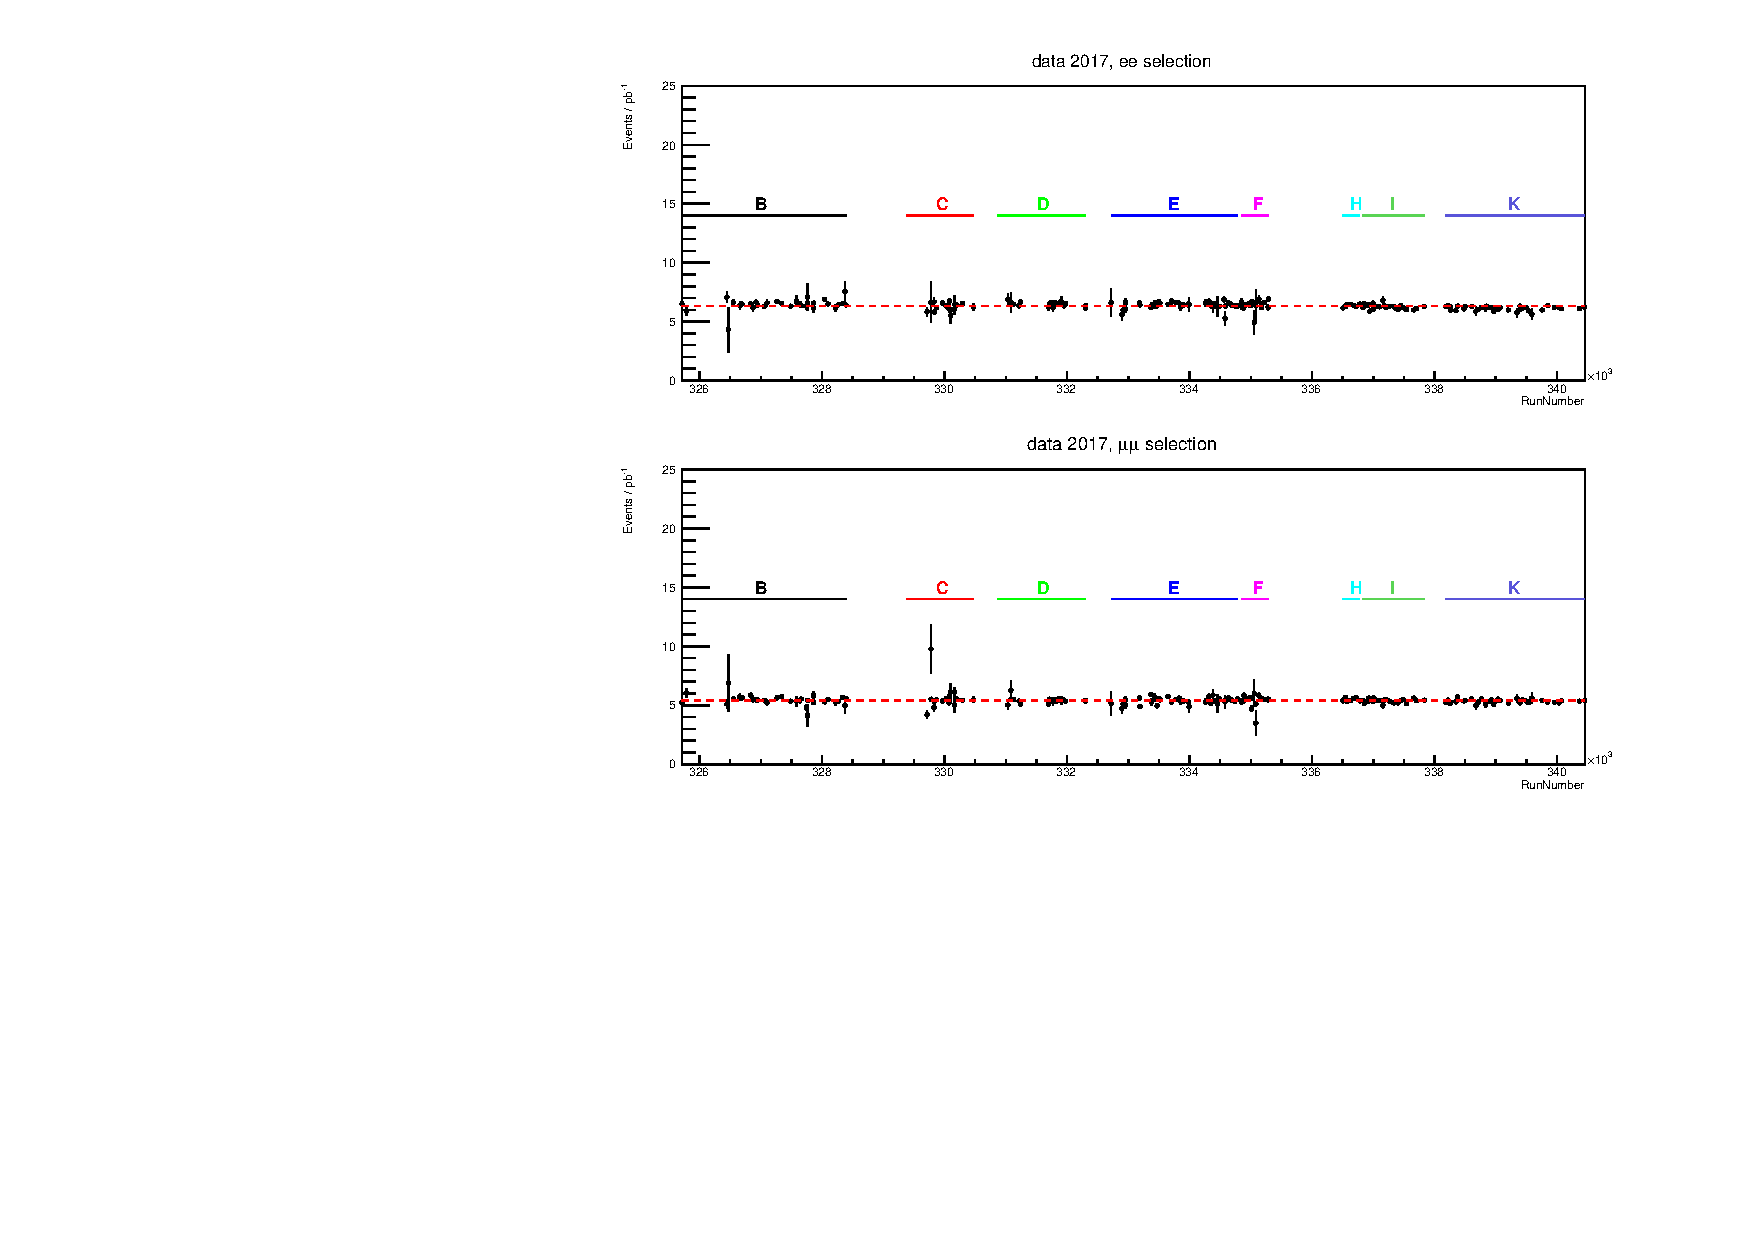
\includegraphics[width=0.48\textwidth]{figures/ci/dataMc/compare_data_yields2017.pdf}}}
\subfloat[][]{{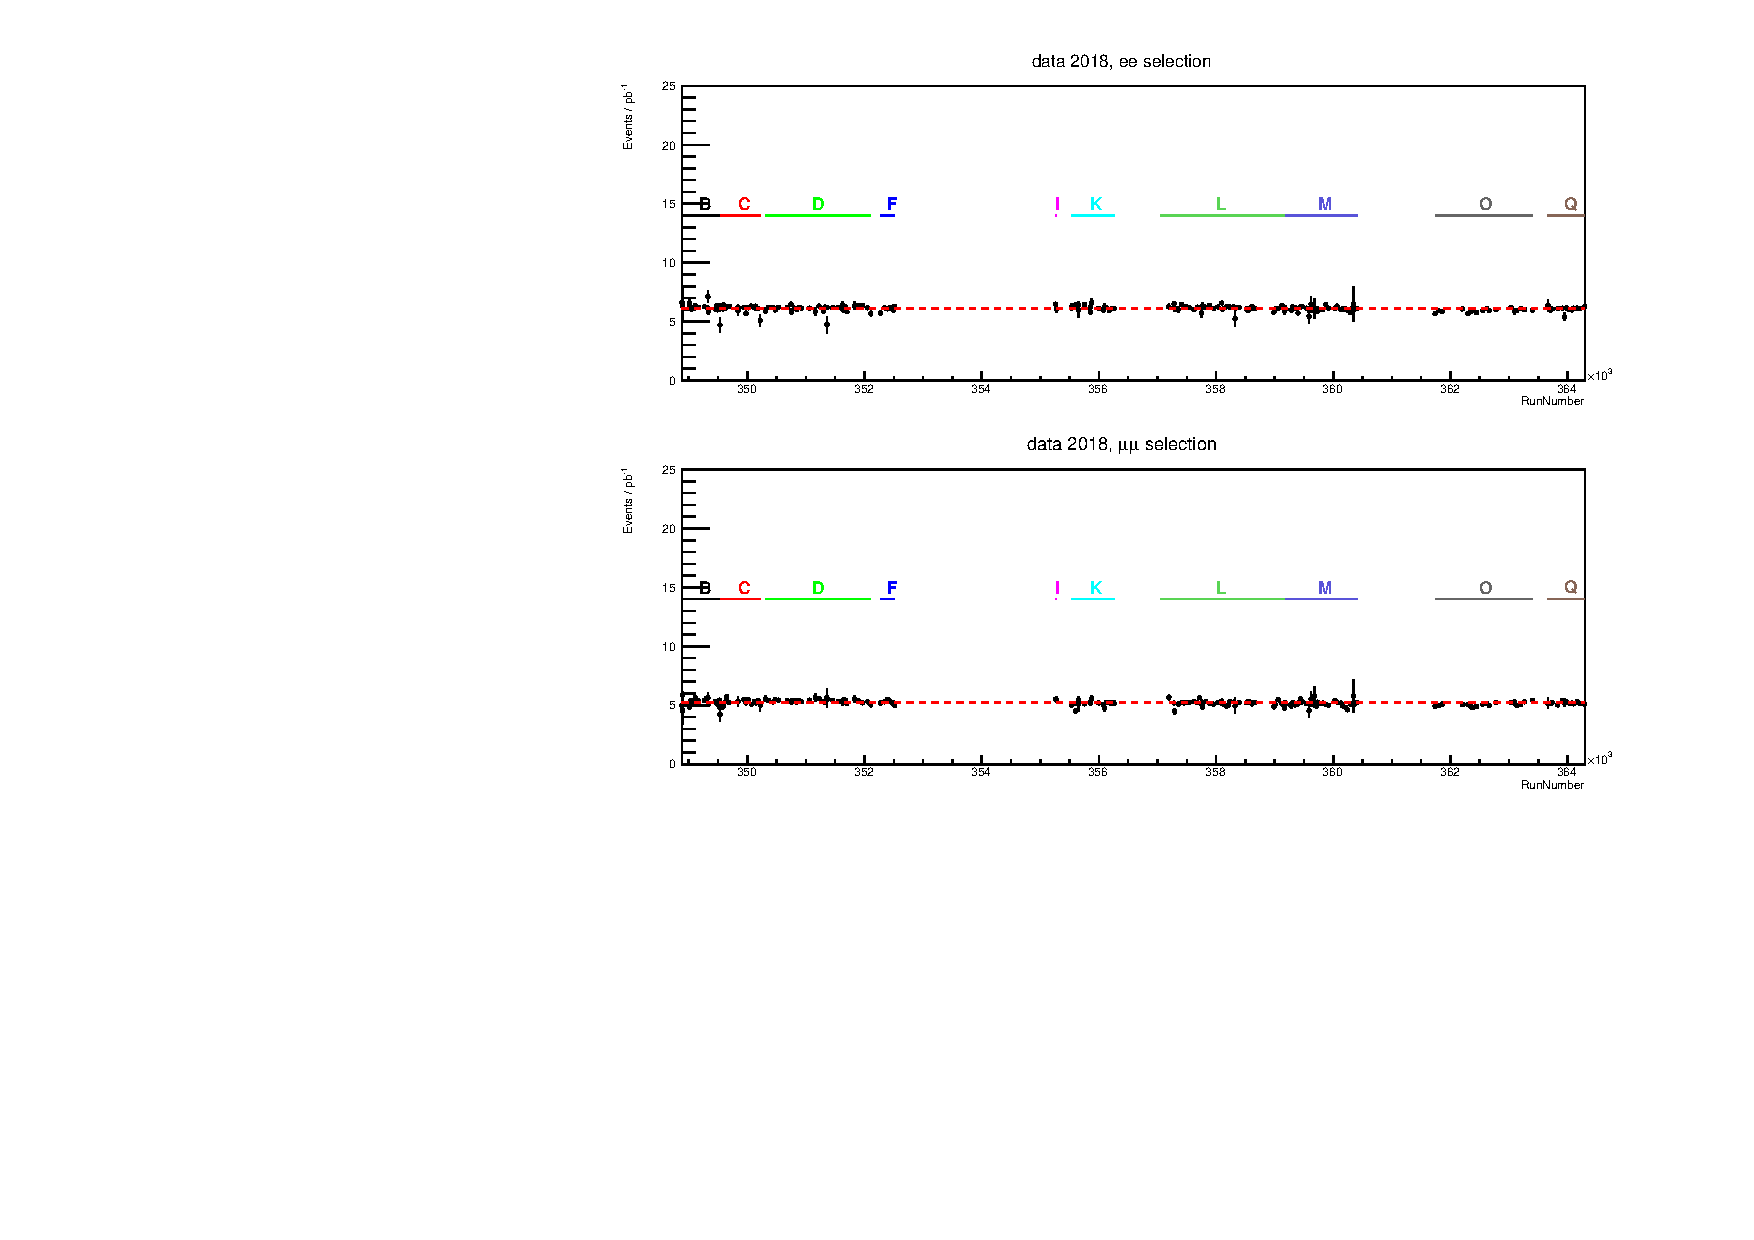
\includegraphics[width=0.48\textwidth]{figures/ci/dataMc/compare_data_yields2018.pdf}}}
\caption{Data yields for the each run period for the inclusive $ee$ (above) and $\mu\mu$ (below) selections.}
\label{fig:ciYields}
\end{figure}
\clearpage

\subsection{Simulation}

This analysis uses simulated invariant-mass distributions for three purposes:
\begin{enumerate}
    \item Modeling the CI signal. This is done using simulated DY events, reweighted to include interference and direct production from a contact interaction.
    \item Testing a variety of choices made during the analysis. In particular, with respect to choosing a functional form that matches the expected background shape and with respect to choosing the control and signal regions.
    \item Measuring the impact of experimental and theoretical uncertainties on the results.
\end{enumerate}

All simulation-based background contributions are scaled by their respective cross-sections and summed to obtain the simulated background $m_{\ell\ell}$ distribution.
The main simulated backgrounds in decreasing order of contribution to the full mass spectrum are: Drell--Yan (DY), top-quark pair ($t\bar{t}$), single-top-quark and diboson production.
The multi-jet and $W+$jets processes in the dielectron channel are estimated from the data using the matrix method similarly to Ref.~\cite{EXOT-2016-05}. The contribution of such processes to the analysis is estimated using a likelihood fit.
The same processes in the dimuon channel, as well as processes with $\tau$-leptons in both channels, have a negligible impact and are not considered.
The Monte Carlo (MC) event generators for the hard-scattering process and the programs used for parton showering are listed in Table~\ref{tab:MC} with their respective parton distribution functions (PDFs).
`Afterburner' generators such as \textsc{Photos}~\cite{Golonka:2005pn} for the final-state photon radiation (FSR) modeling, \textsc{MadSpin}~\cite{Artoisenet:2012st} to preserve top-quark spin correlations, and \textsc{EvtGen}~\cite{Lange:2001uf} for the modeling of $c$- and $b$-hadron decays, are also included in the simulation.

\begin{table}[htbp]
\centering
\caption{The programs and PDFs used to generate the hard-scatter matrix element (ME) and to simulate parton showering (PS) in the signal and background processes.
The top-quark mass is set to 172.5 GeV.}
{\scriptsize
\begin{tabular}{lll}
\toprule
Background Process & ME Generator and ME PDFs & PS and non-perturbative effect with PDFs \\\hline
NLO Drell--Yan & \POWHEGBOX~\cite{Alioli:2010xd,Frixione:2007vw}, CT10~\cite{ct10}, \textsc{Photos} & \PYTHIAV{v8.186}~\cite{pythia8}, CTEQ6L1~\cite{ATL-PHYS-PUB-2014-021,Stump:2003yu}, \textsc{EvtGen1.2.0} \\
$t\bar{t}$  & \POWHEGBOX, NNPDF3.0NLO~\cite{Ball:2014uwa} & \PYTHIAV{v8.230}, NNPDF23LO~\cite{Ball:2012cx}, \textsc{EvtGen1.6.0} \\
Single top $s$-channel, $Wt$& \POWHEGBOX, NNPDF3.0NLO & \PYTHIAV{v8.230}, NNPDF23LO, \textsc{EvtGen1.6.0} \\
Single top $t$-channel & \POWHEGBOX, NNPDF3.04fNLO, \textsc{MadSpin} & \PYTHIAV{v8.230}, NNPDF23LO, \textsc{EvtGen1.6.0}  \\
Diboson ($WW$, $WZ$ and $ZZ$) & \SHERPA 2.1.1~\cite{Gleisberg:2008ta}, CT10 &\SHERPA 2.1.1, CT10  \\\hline
Signal Process & & \\\hline
LO Drell--Yan & \PYTHIAV{v8.186}, NNPDF23LO  &  \PYTHIAV{v8.186}, NNPDF23LO, \textsc{EvtGen1.2.0} \\
LO CI & \PYTHIAV{v8.186}, NNPDF23LO  &  \PYTHIAV{v8.186}, NNPDF23LO, \textsc{EvtGen1.2.0} \\
\bottomrule
\end{tabular}
}
\normalsize
\label{tab:MC}
\end{table}
SOFT-2010-01



The DY~\cite{ATL-PHYS-PUB-2016-003} and diboson~\cite{ATL-PHYS-PUB-2016-002} samples were generated in slices of dilepton mass to increase the sample statistics in the high-mass region.
Next-to-next-to-leading-order (NNLO) corrections in quantum chromodynamic (QCD) theory, and next-to-leading-order (NLO) corrections in electroweak (EW) theory, were calculated and applied to the DY events.
The corrections were computed with {\textsc{VRAP}} v0.9~\cite{vrap} and the CT14 NNLO PDF set~\cite{CT14} in the case of QCD effects, whereas they were computed with {\textsc{MCSANC}}~\cite{MCSANC} in the case of quantum electrodynamic effects due to initial-state radiation, interference between initial- and final-state radiation and Sudakov logarithm single-loop corrections.
These are calculated as mass-dependent K-factors, and reweight simulated events before reconstruction.
The top-quark samples~\cite{ATL-PHYS-PUB-2016-020} are normalised to the cross-sections calculated at NNLO in QCD including resummation of the next-to-next-to-leading logarithmic soft gluon terms as provided by \textsc{Top++}2.0~\cite{Czakon:2011xx}.

% Scale factors
The simulated data is weighted by a number of \emph{scale factors}, such that it more accurately represents reality.
These are listed here:
\begin{itemize}
	\item Pile-up reweighting weights.
	\item Mass dependant $K$-factors account for differences in the total cross-section if higher order calculations are available for a given process compared to the order available in the MC samples. In case of the LO and NLO DY samples, the SFs provide corrections for higher-order QCD, EW and photon-induced (PI) effects.
	\item Experimental scale factors for leptons:
	\begin{itemize}
		\item Electrons: Reconstruction, trigger, isolation and identification scales factors are applied.
		\item Muons: Reconstruction, trigger, isolation and TTVA scale factors are applied.
	\end{itemize}
	\item Trigger scale factors according to the specific channel.
\end{itemize}

All fully simulated event samples include the effect of multiple $pp$ interactions in the same or neighbouring bunch crossings.
These effects are collectively referred to as pile-up.
The simulation of pile-up collisions was performed with \PYTHIAV{v8.186} using the ATLAS A3 set of tuned parameters~\cite{ATL-PHYS-PUB-2016-017} and the NNPDF23LO PDF set, and weighted to reproduce the average number of pile-up interactions per bunch crossing observed in data.
The generated events were passed through a full detector simulation~\cite{SOFT-2010-01} based on\ \GEANT~4~\cite{geant}.

In order to reduce statistical uncertainties, a large additional DY sample is used where the detector response is modeled by smearing the dilepton invariant-mass with mass-dependent acceptance and efficiency corrections, instead of using the CPU-intensive \GEANT~4 simulation.
The relative dilepton mass resolution used in the smearing procedure is defined as $(m_{\ell\ell}-m_{\ell\ell}^\mathrm{true})/m_{\ell\ell}^\mathrm{true}$, where $m_{\ell\ell}^\mathrm{true}$ is the generated dilepton mass at Born level before FSR.
The mass resolution is parameterised as a sum of a Gaussian distribution, which describes the detector response, and a Crystal Ball function composed of a secondary Gaussian distribution with a power-law low-mass tail,
which accounts for bremsstrahlung effects or for the effect of poor resolution in the muon momentum at high \pt.
The parameterisation of the relative dilepton mass resolution as a function of $m_{\ell\ell}^\mathrm{true}$ is determined by a fit of the function described above to simulated DY events at NLO.
A similar procedure is used to produce a mass-smeared $t\bar{t}$ sample.
These two samples replace the equivalent ones produced with the full detector simulation wherever applicable in the remainder of the analysis.
The number of events in these samples is more than 55 times the number of events in data.
These samples would have been difficult to produce with the full detector simulation because of the large number of events required and the limited computing resources.

Signal $m_{\ell\ell}$ distribution shapes are obtained by a matrix-element reweighting~\cite{EXOT-2016-05} of the leading-order (LO) DY samples generated in slices of dilepton mass.
This reweighting includes the full interference between the non-resonant signal and the background DY process.
The weight function is the ratio of the analytical matrix-elements of the full CI (including the DY component) and the DY process only, both at LO.
It takes as an input the generated dilepton mass at Born level before FSR, the incoming quarks' flavour and the CI model parameters ($\Lambda$, chirality states and the interference structure).
These weights are applied to the LO DY events to transform these into the CI signal shapes, in steps of $2$~TeV between $\Lambda=12$~TeV and $\Lambda=100$~TeV.
Dilepton mass-dependent higher-order QCD production corrections for the signals are computed with the same methodology as for the DY background, correcting from LO to NNLO.
Similarly, electroweak corrections for the signals are applied in the CI reweighting along with the interference effects, correcting from LO to NLO.
These signal shapes are used for optimisations as well as for calculations of the cross-section and acceptance times efficiency.

Several distributions of kinematic variables are provided in the following figures.
First the invariant mass distributions are shown in in Figure \ref{fig:ciMassMcPlot}.
These plots show the distribution of simulated events along with data events for both \ee and \mm selections.
Several representative contact interaction shapes are included for reference.
Looking at the simulation, these plots clearly show the relative composition of the background distributions.
The plots of the \ee selection additionally include the multi-jet and $W+$jets background.
The following figures show some kinematic variables for each selection.
Fully simulated resonant signals are included in these as illustrations, as the CI signal is reweighted only in the invariant-mass distribution.

\afterpage{
\begin{figure}[h!]
\captionsetup[subfigure]{position=b}
\centering
 \begin{minipage}[b]{.45\linewidth}
    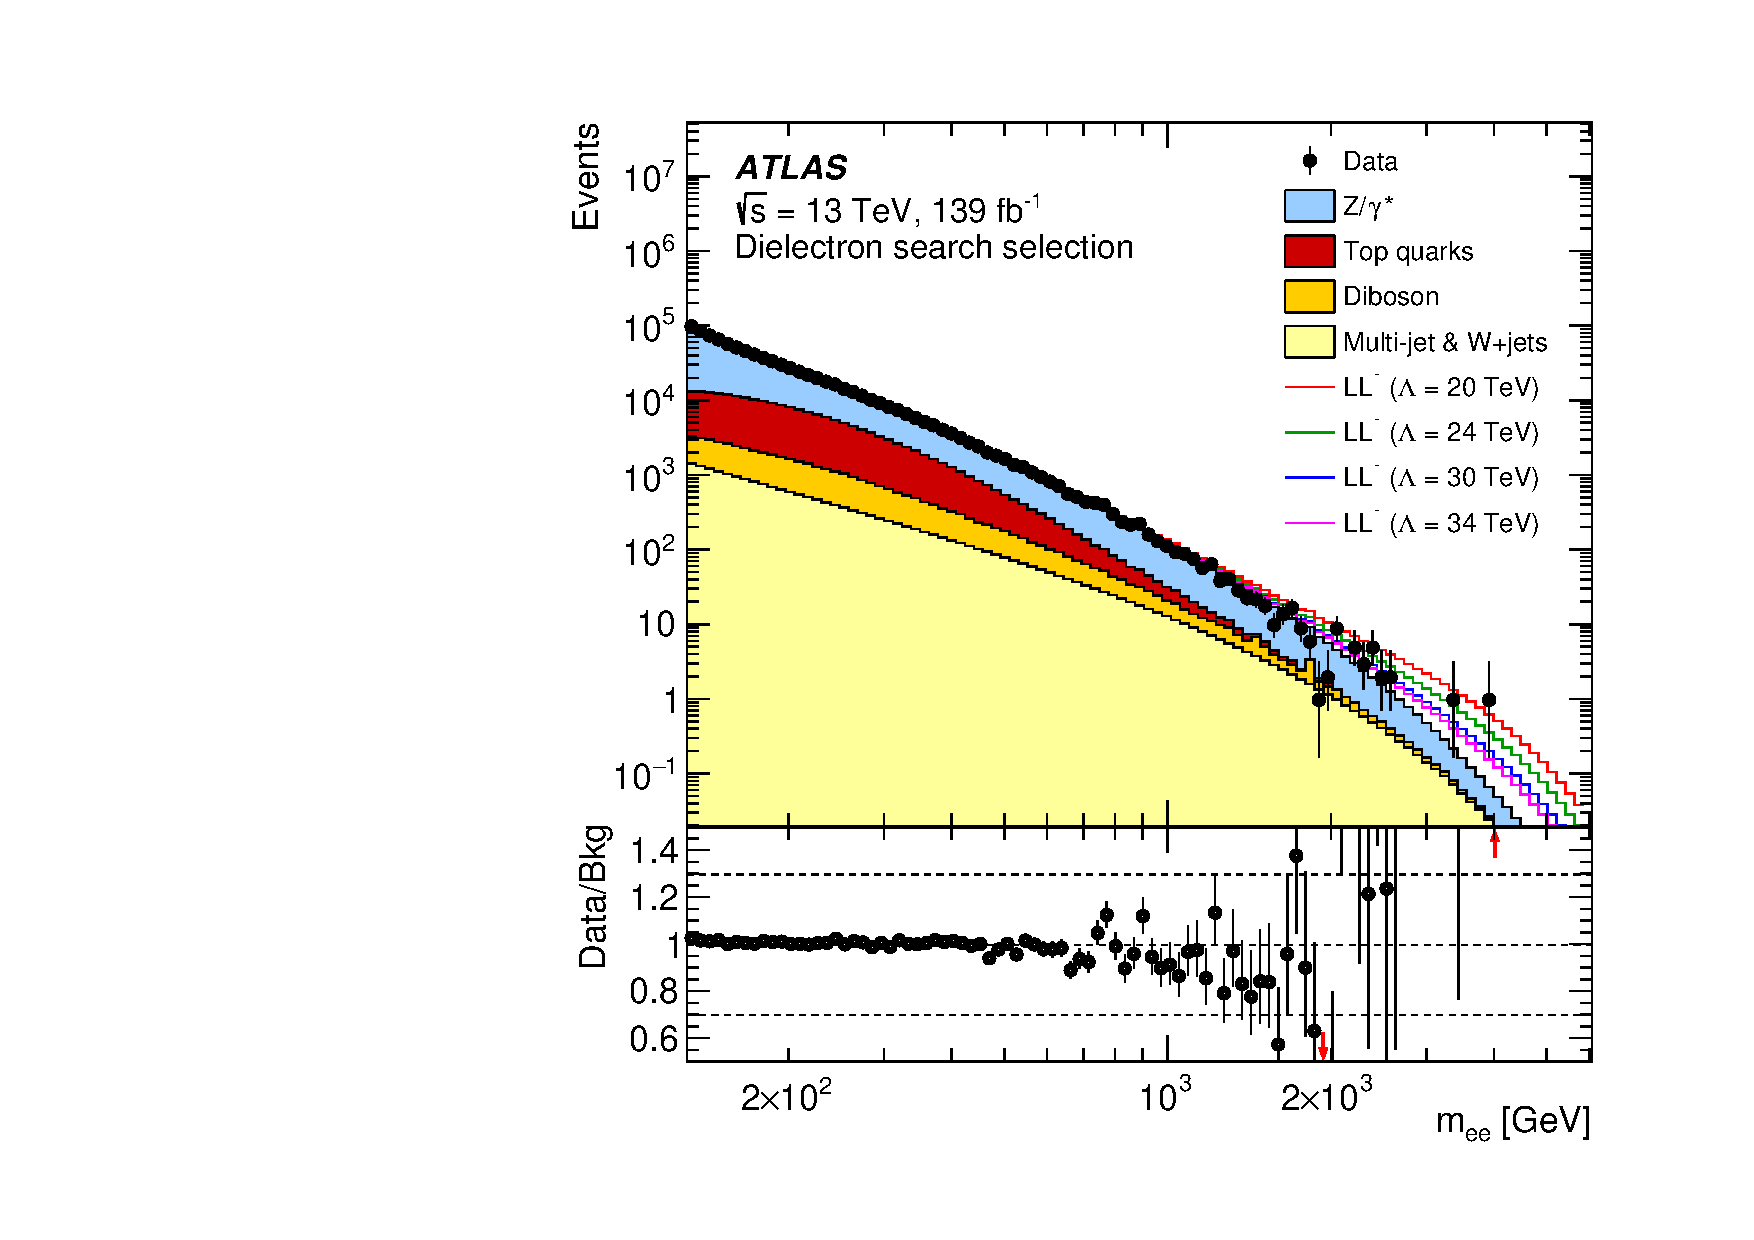
\includegraphics[width=1\textwidth]{figures/ci/dataMc/figaux_05a.pdf}
    \subcaption{}\label{fig:1a}
\end{minipage}
\begin{minipage}[b]{.45\linewidth}
    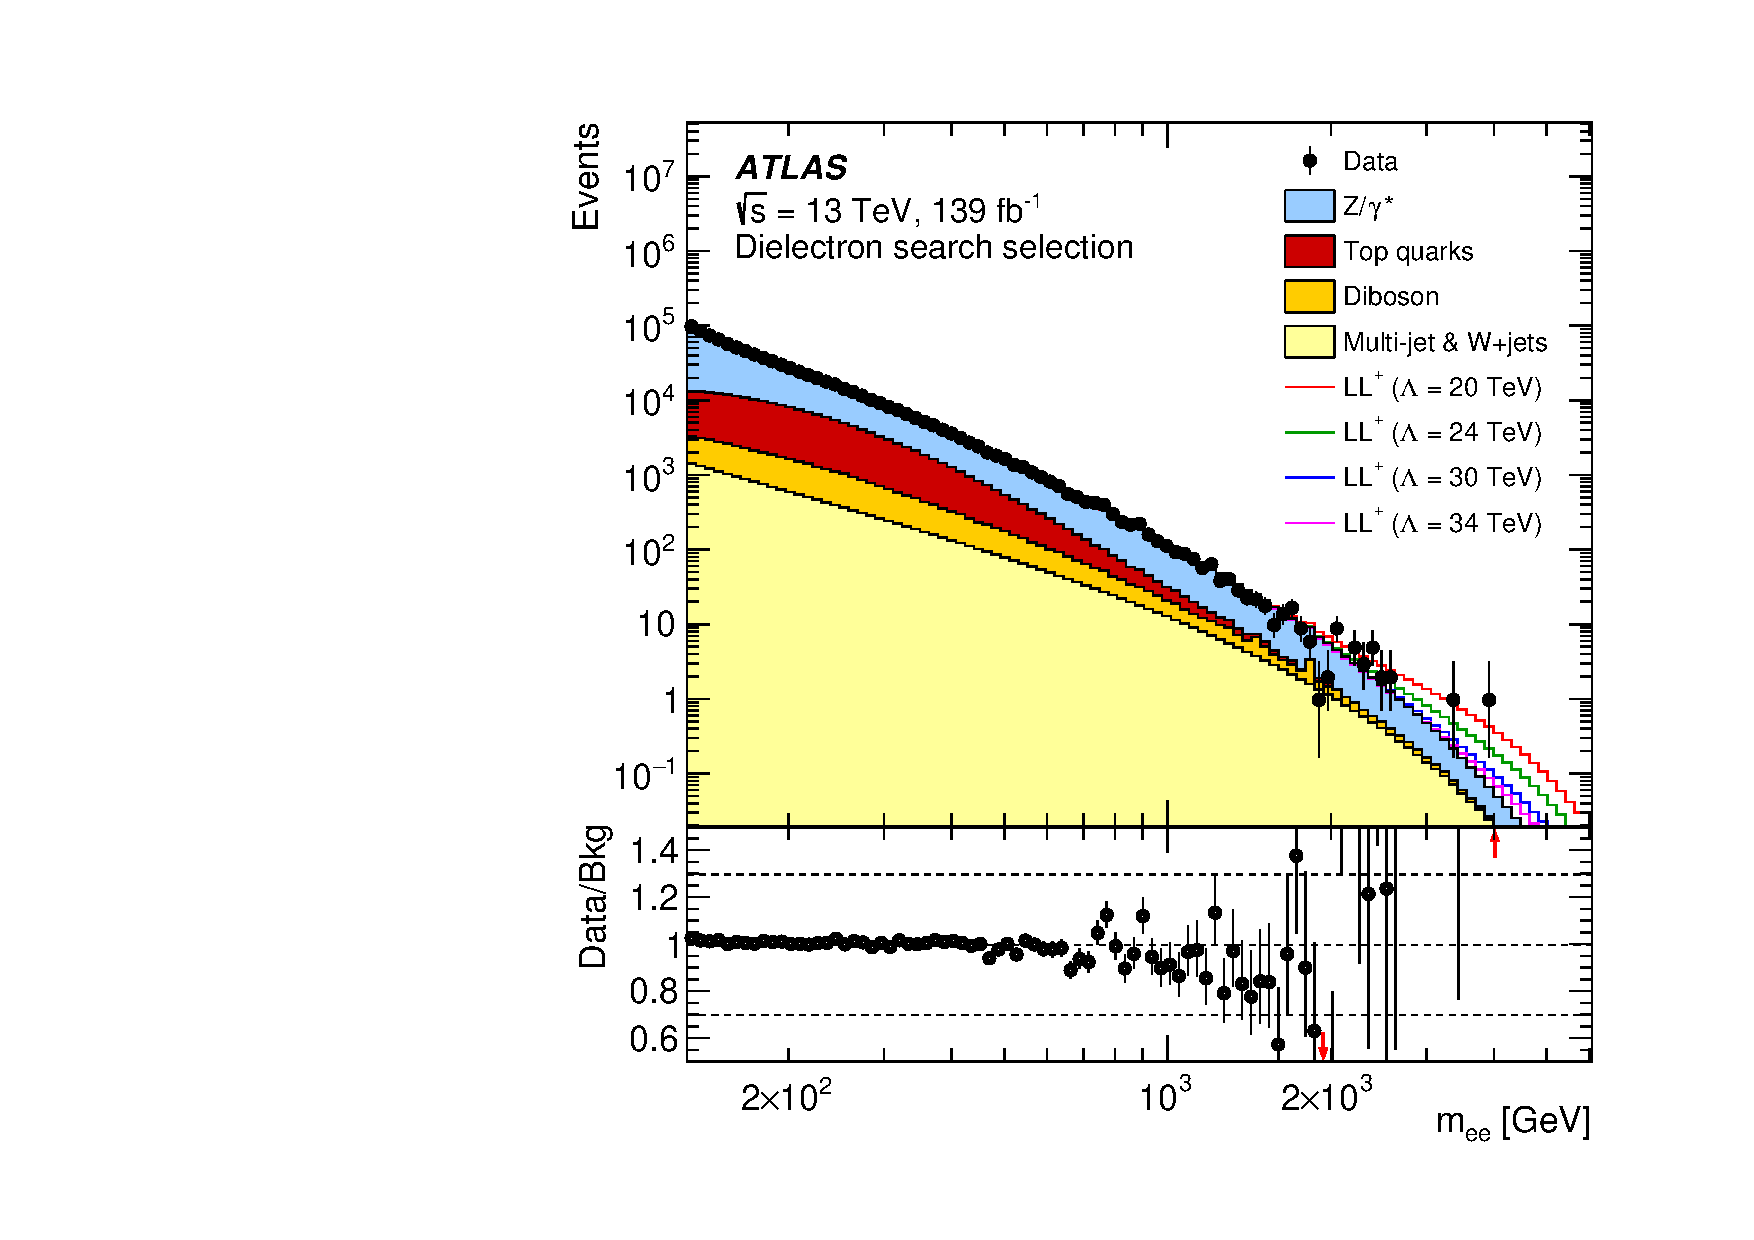
\includegraphics[width=1\textwidth]{figures/ci/dataMc/figaux_05b.pdf}
    \subcaption{}
\end{minipage} \\
\begin{minipage}[b]{.45\linewidth}
    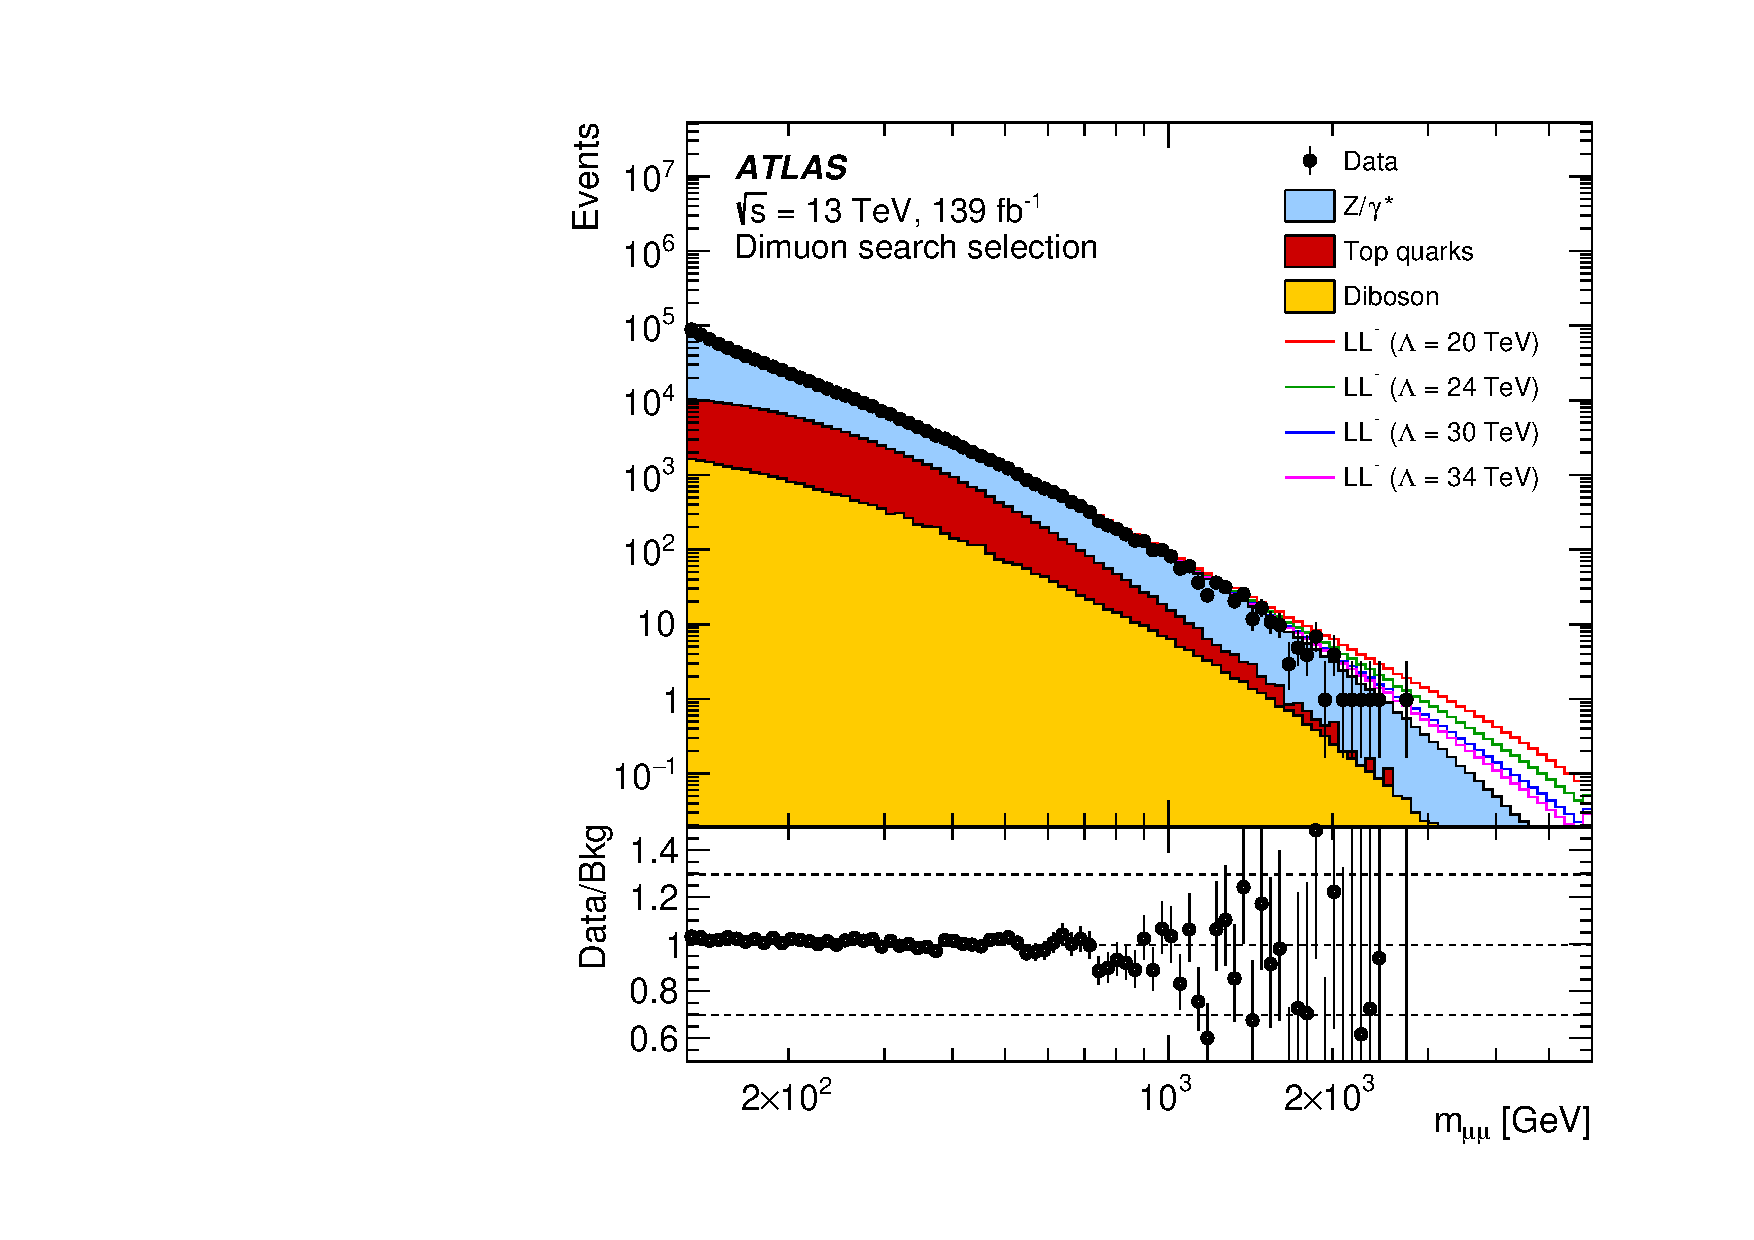
\includegraphics[width=1\textwidth]{figures/ci/dataMc/figaux_06a.pdf}
    \subcaption{}
\end{minipage}
\begin{minipage}[b]{.45\linewidth}
    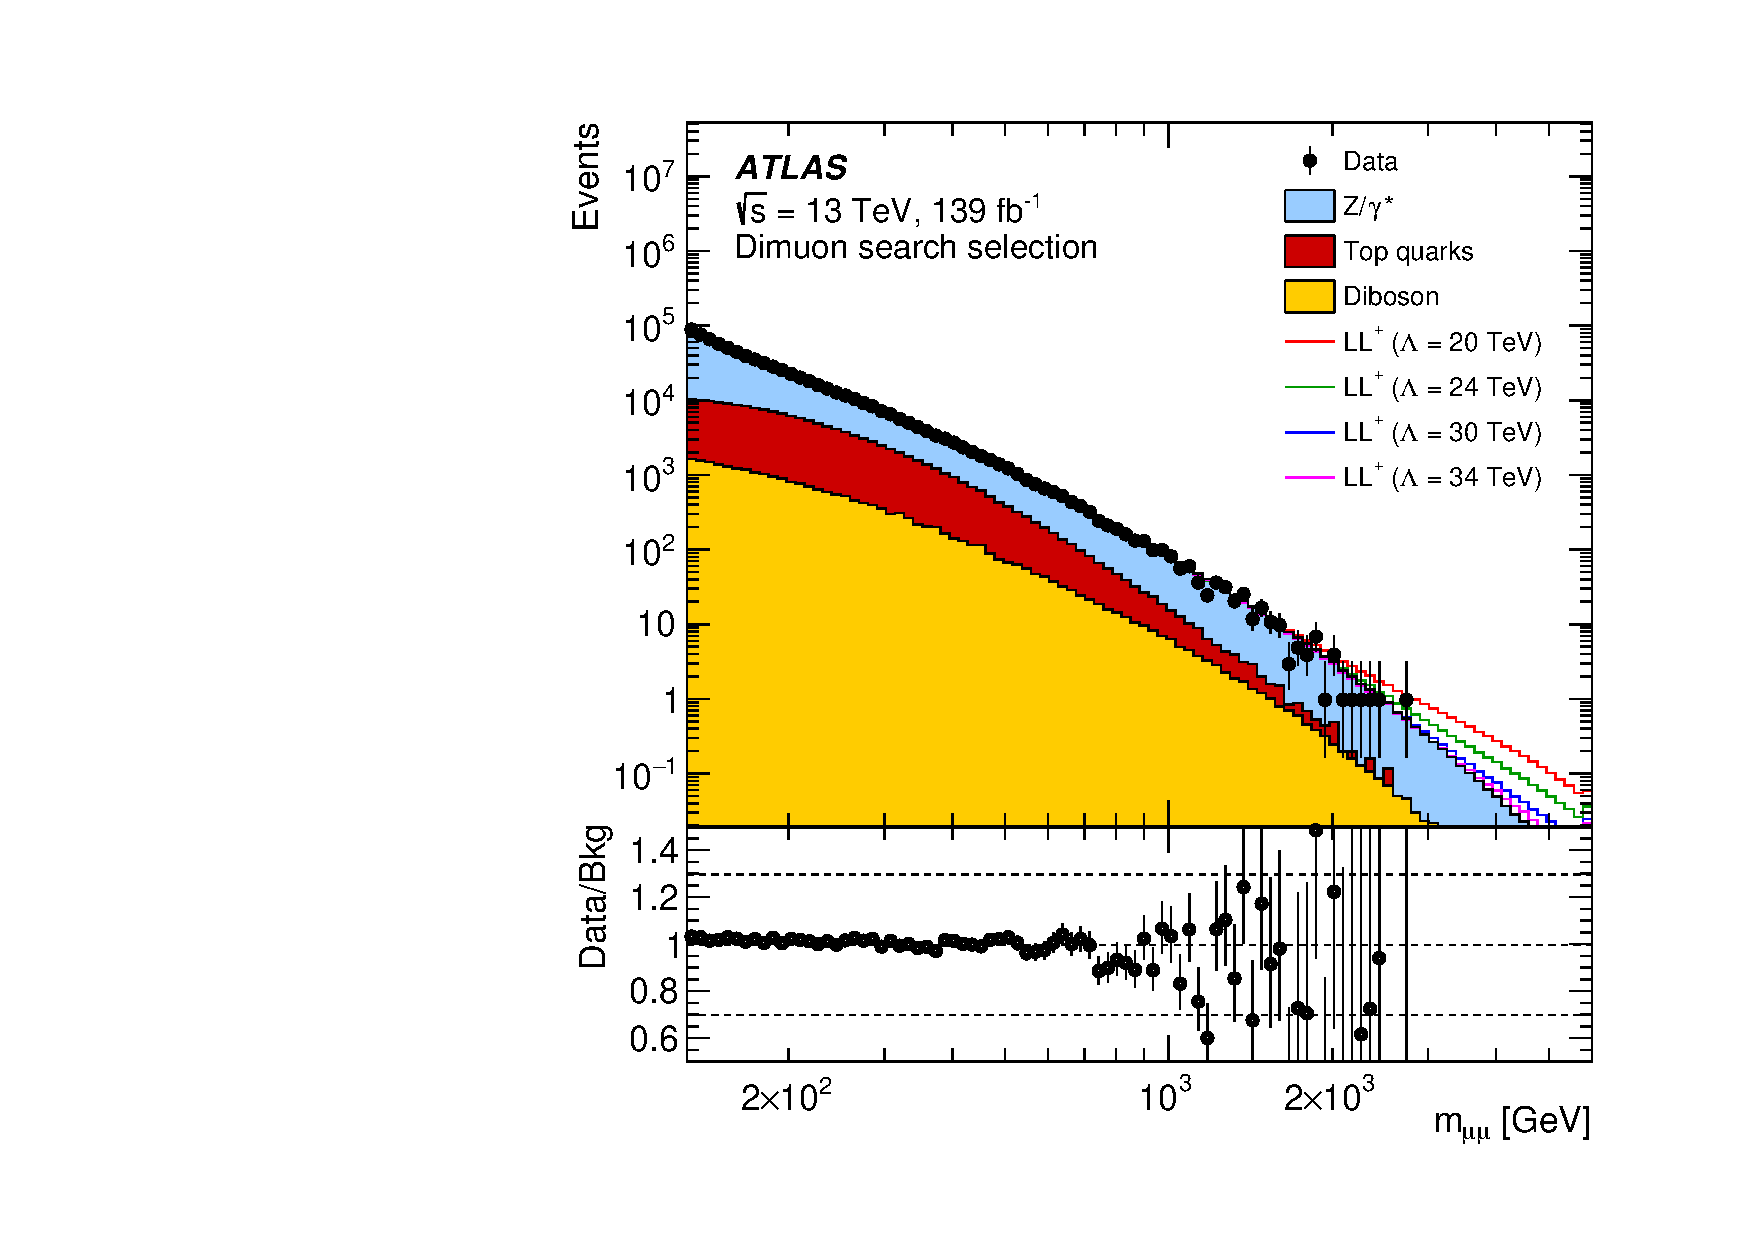
\includegraphics[width=1\textwidth]{figures/ci/dataMc/figaux_06b.pdf}
    \subcaption{}
\end{minipage}
\caption{Invariant-mass distributions in the $ee$ channel (top) and $\mu\mu$ channel (bottom). Plots on the left show selected constructive CI signal shapes imposed on top of the simulated distribution, while plots on the right show the same for destructive CI signal shapes.}
\label{fig:ciMassMcPlot}
\end{figure}
\clearpage
}

\afterpage{
\begin{figure}[h!]
\captionsetup[subfigure]{position=b}
\centering
 \begin{minipage}[b]{.45\linewidth}
    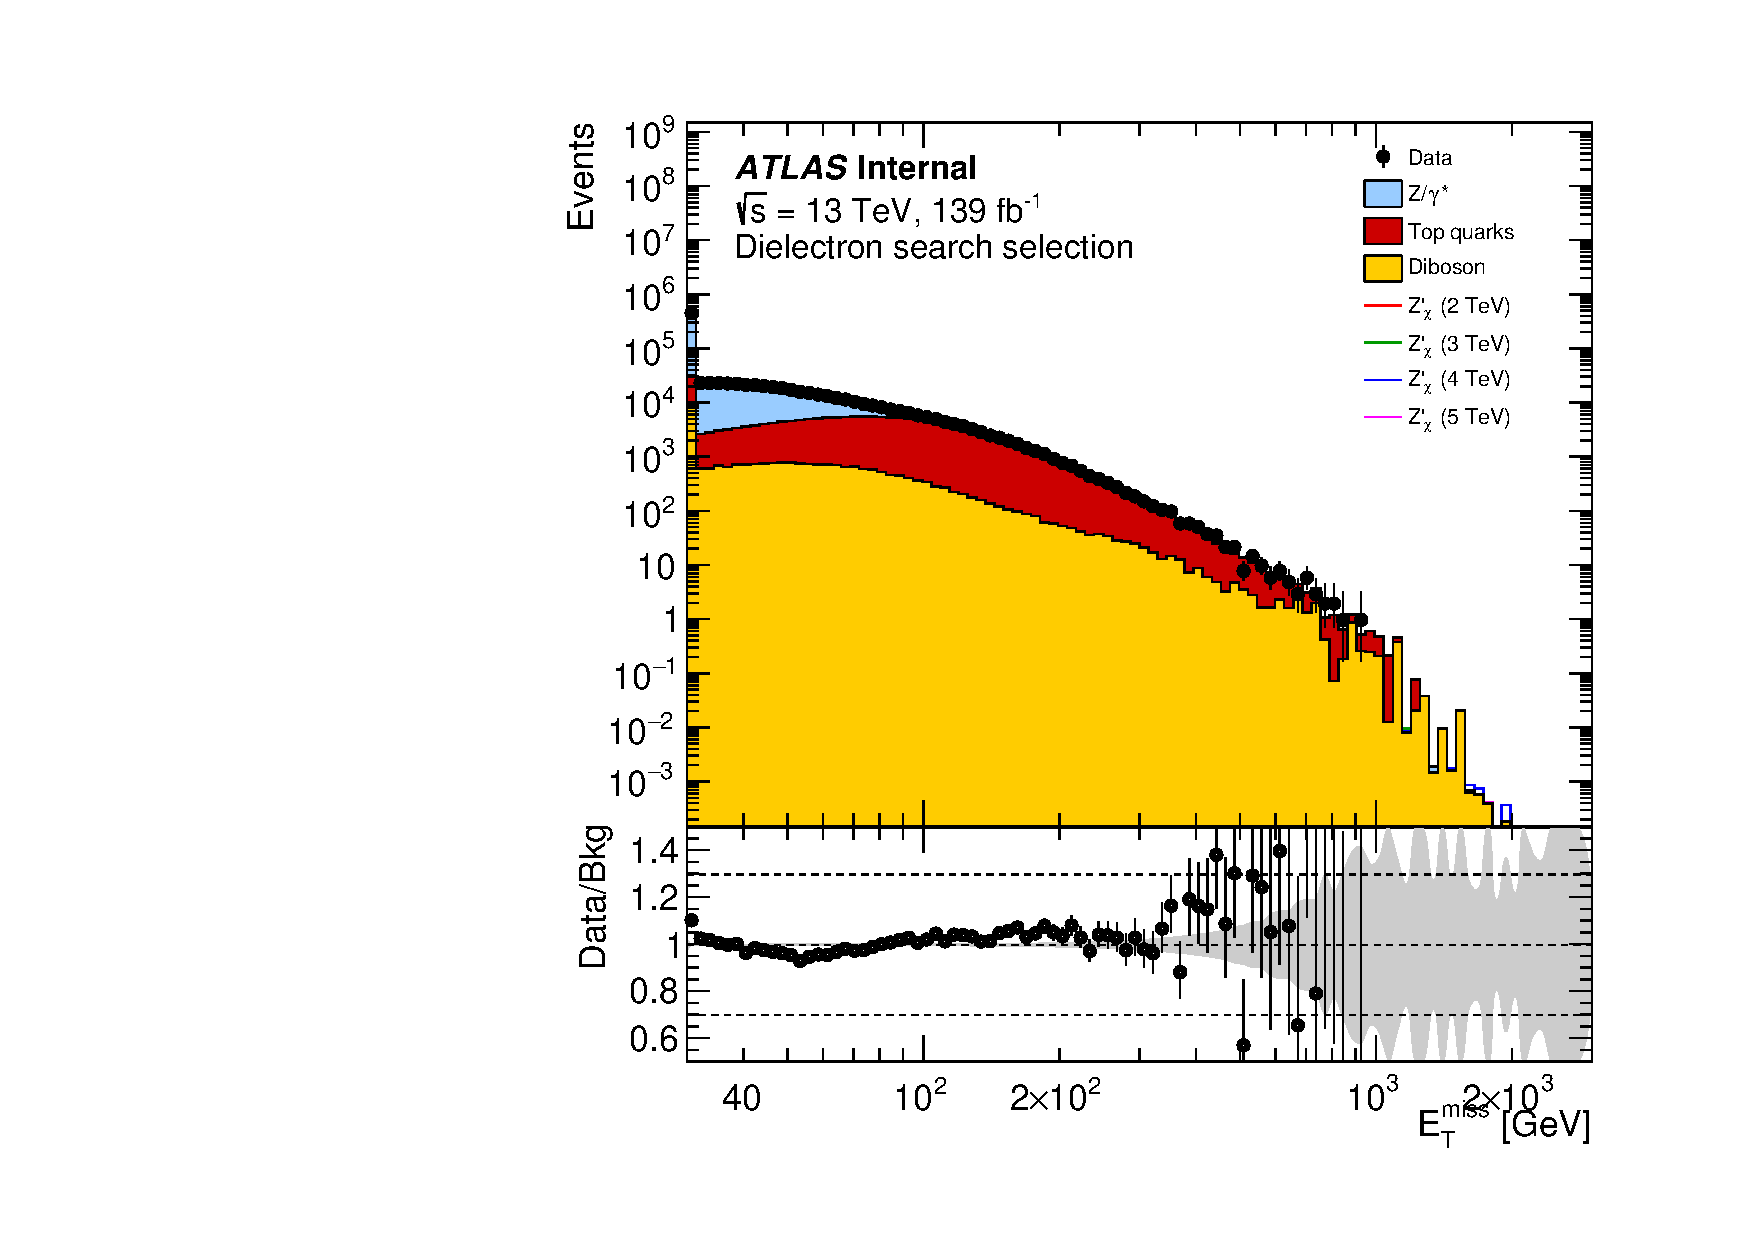
\includegraphics[width=1\textwidth]{figures/ci/dataMc/stacks_mc16e_2015-2018_ee_met_log100.pdf}
    \subcaption{}\label{fig:1a}
\end{minipage}
\begin{minipage}[b]{.45\linewidth}
    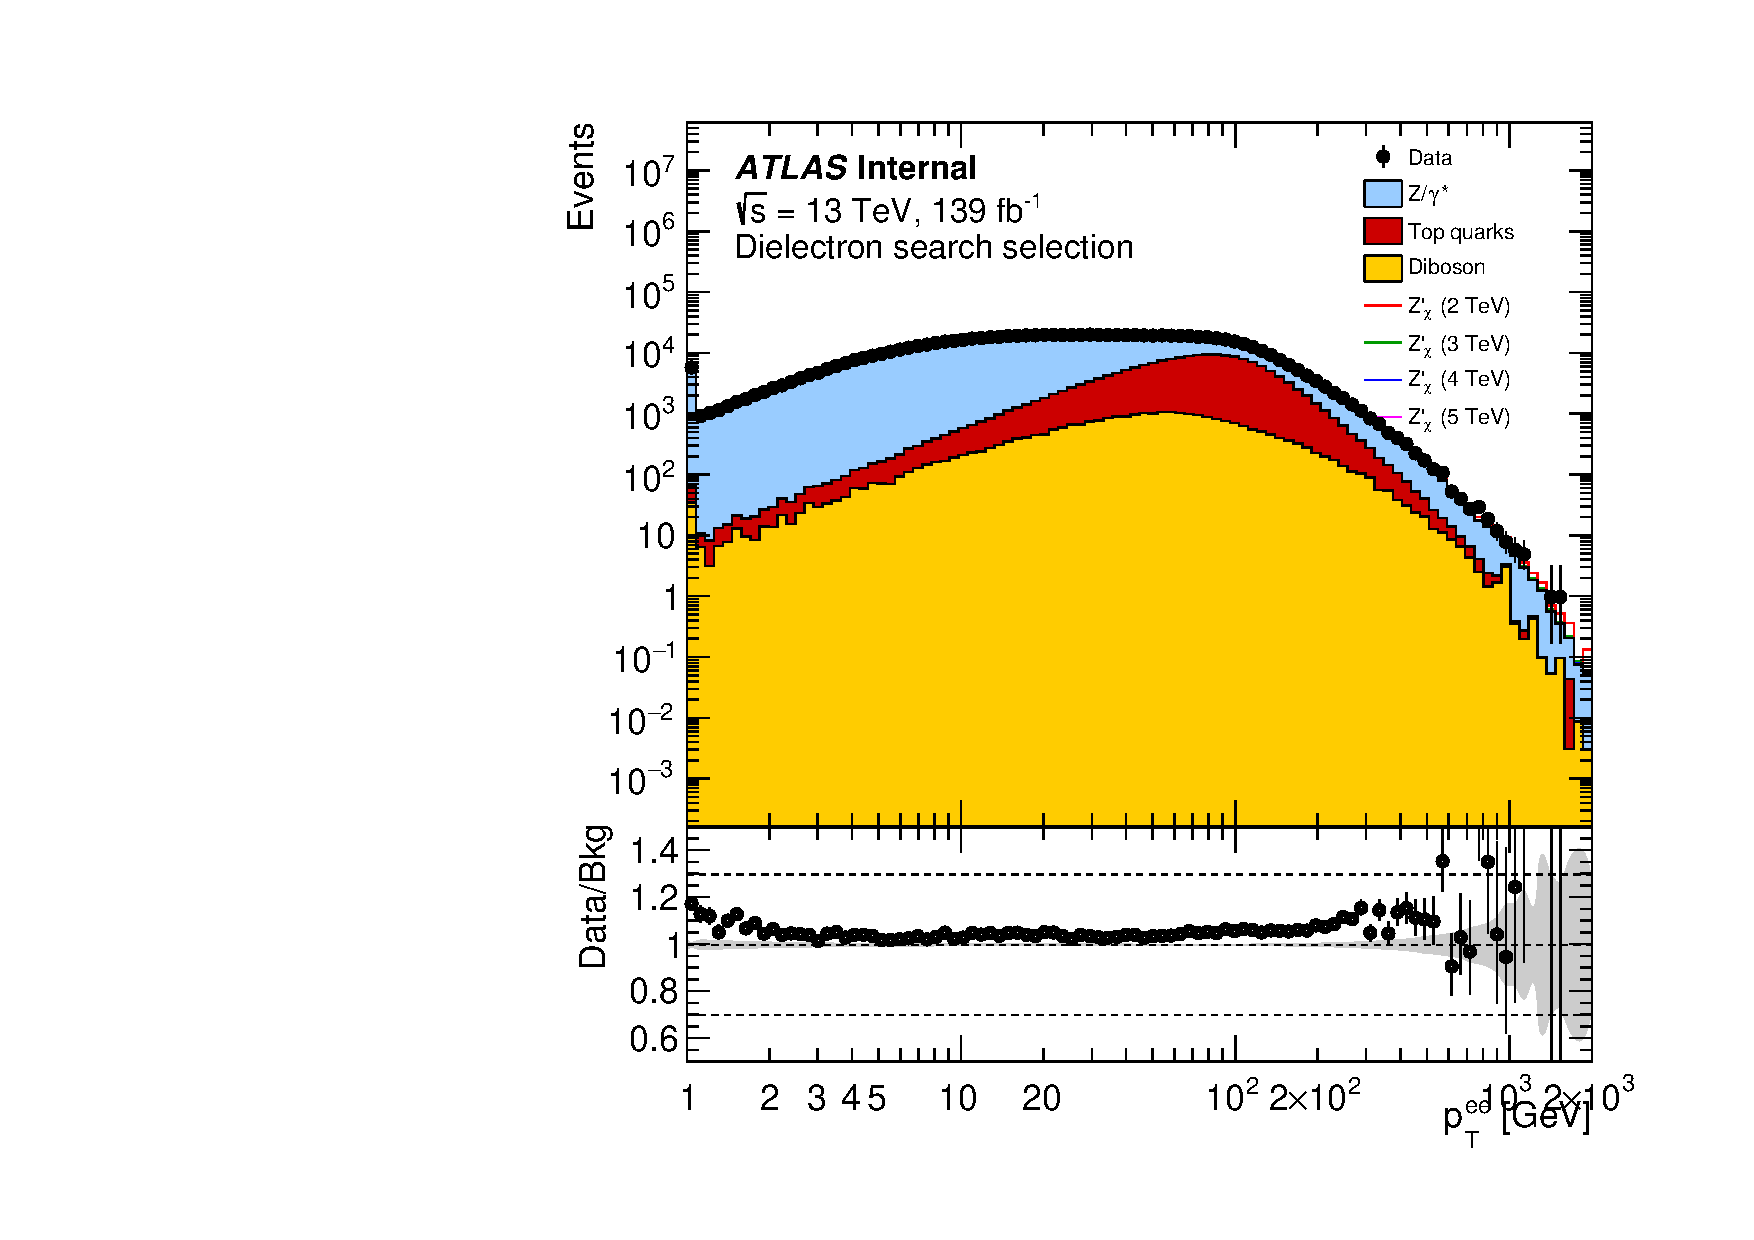
\includegraphics[width=1\textwidth]{figures/ci/dataMc/stacks_mc16e_2015-2018_ee_ptll_log100.pdf}
    \subcaption{}
\end{minipage} \\
\begin{minipage}[b]{.45\linewidth}
    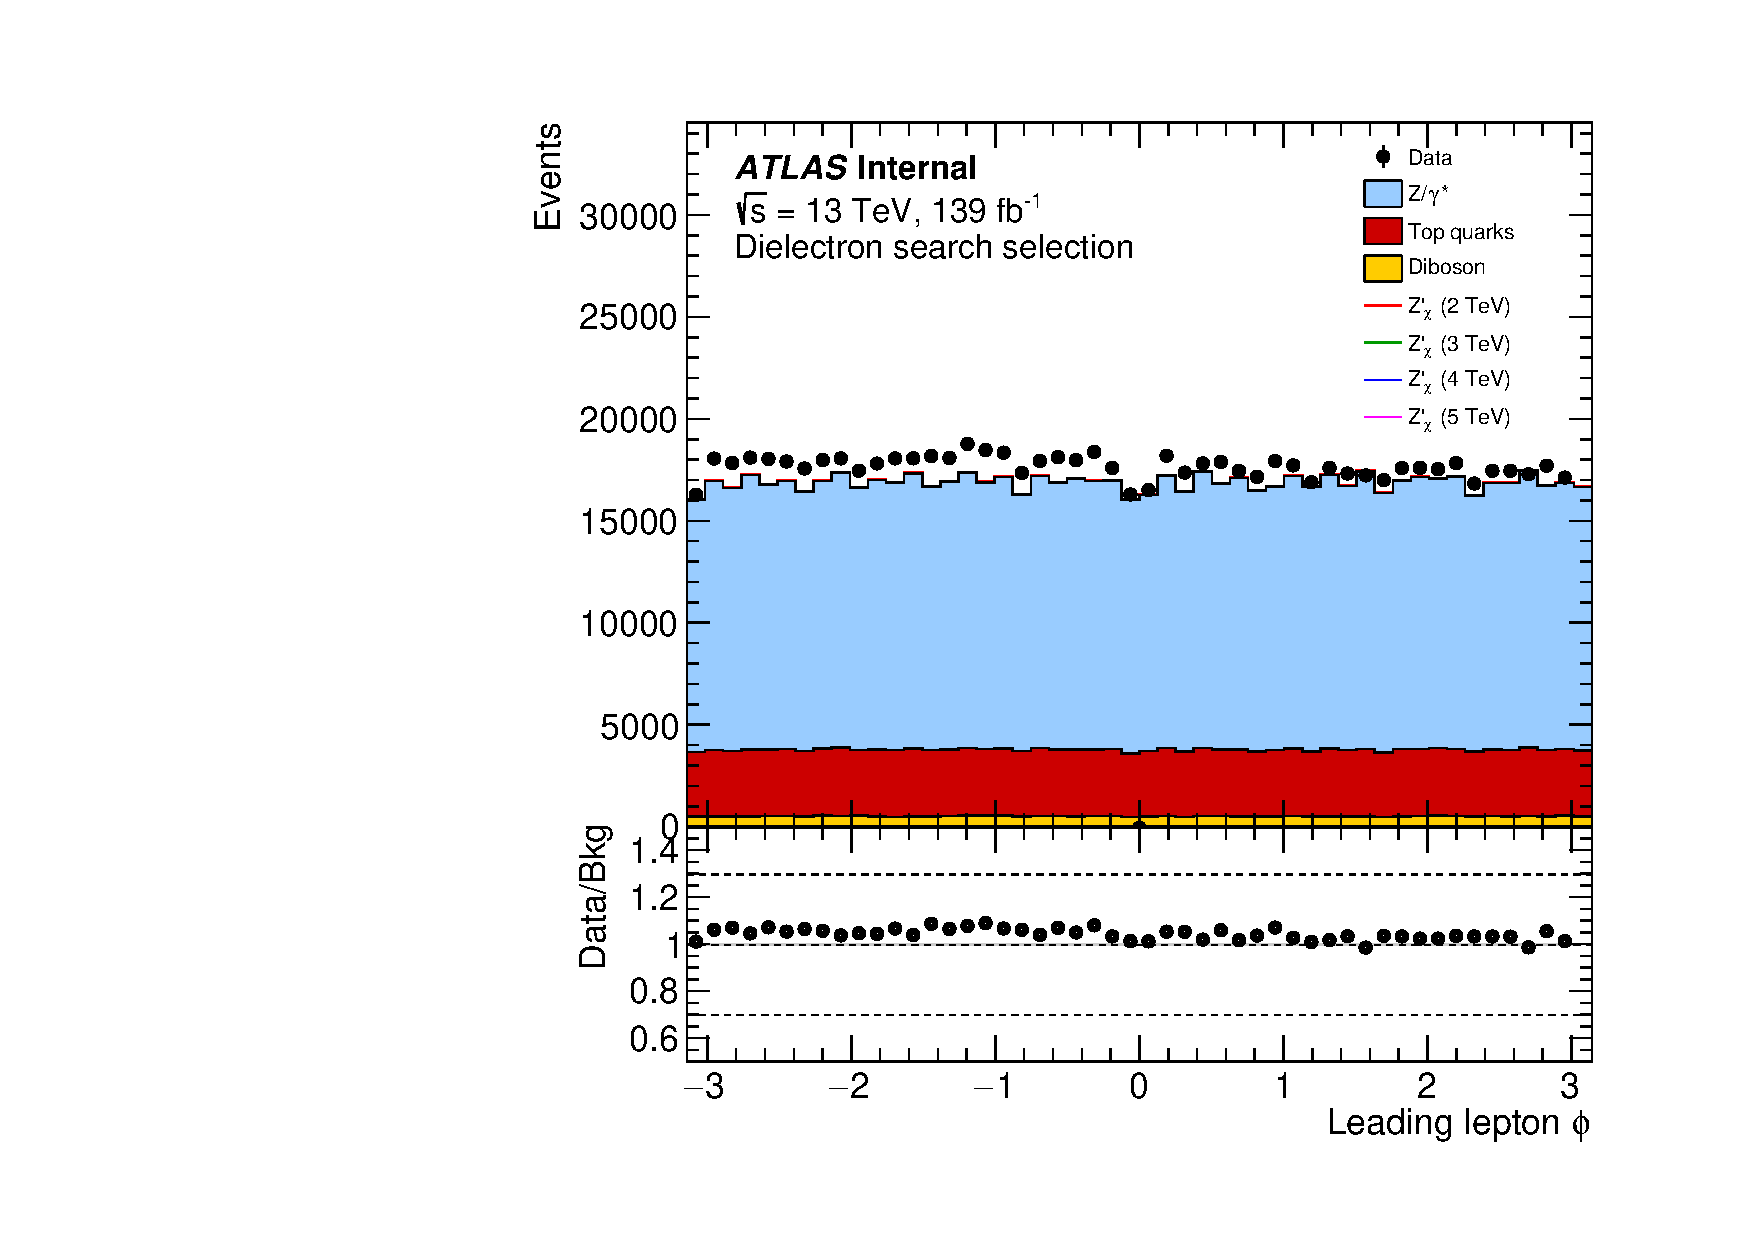
\includegraphics[width=1\textwidth]{figures/ci/dataMc/stacks_mc16e_2015-2018_ee_phi1.pdf}
    \subcaption{}
\end{minipage}
\begin{minipage}[b]{.45\linewidth}
    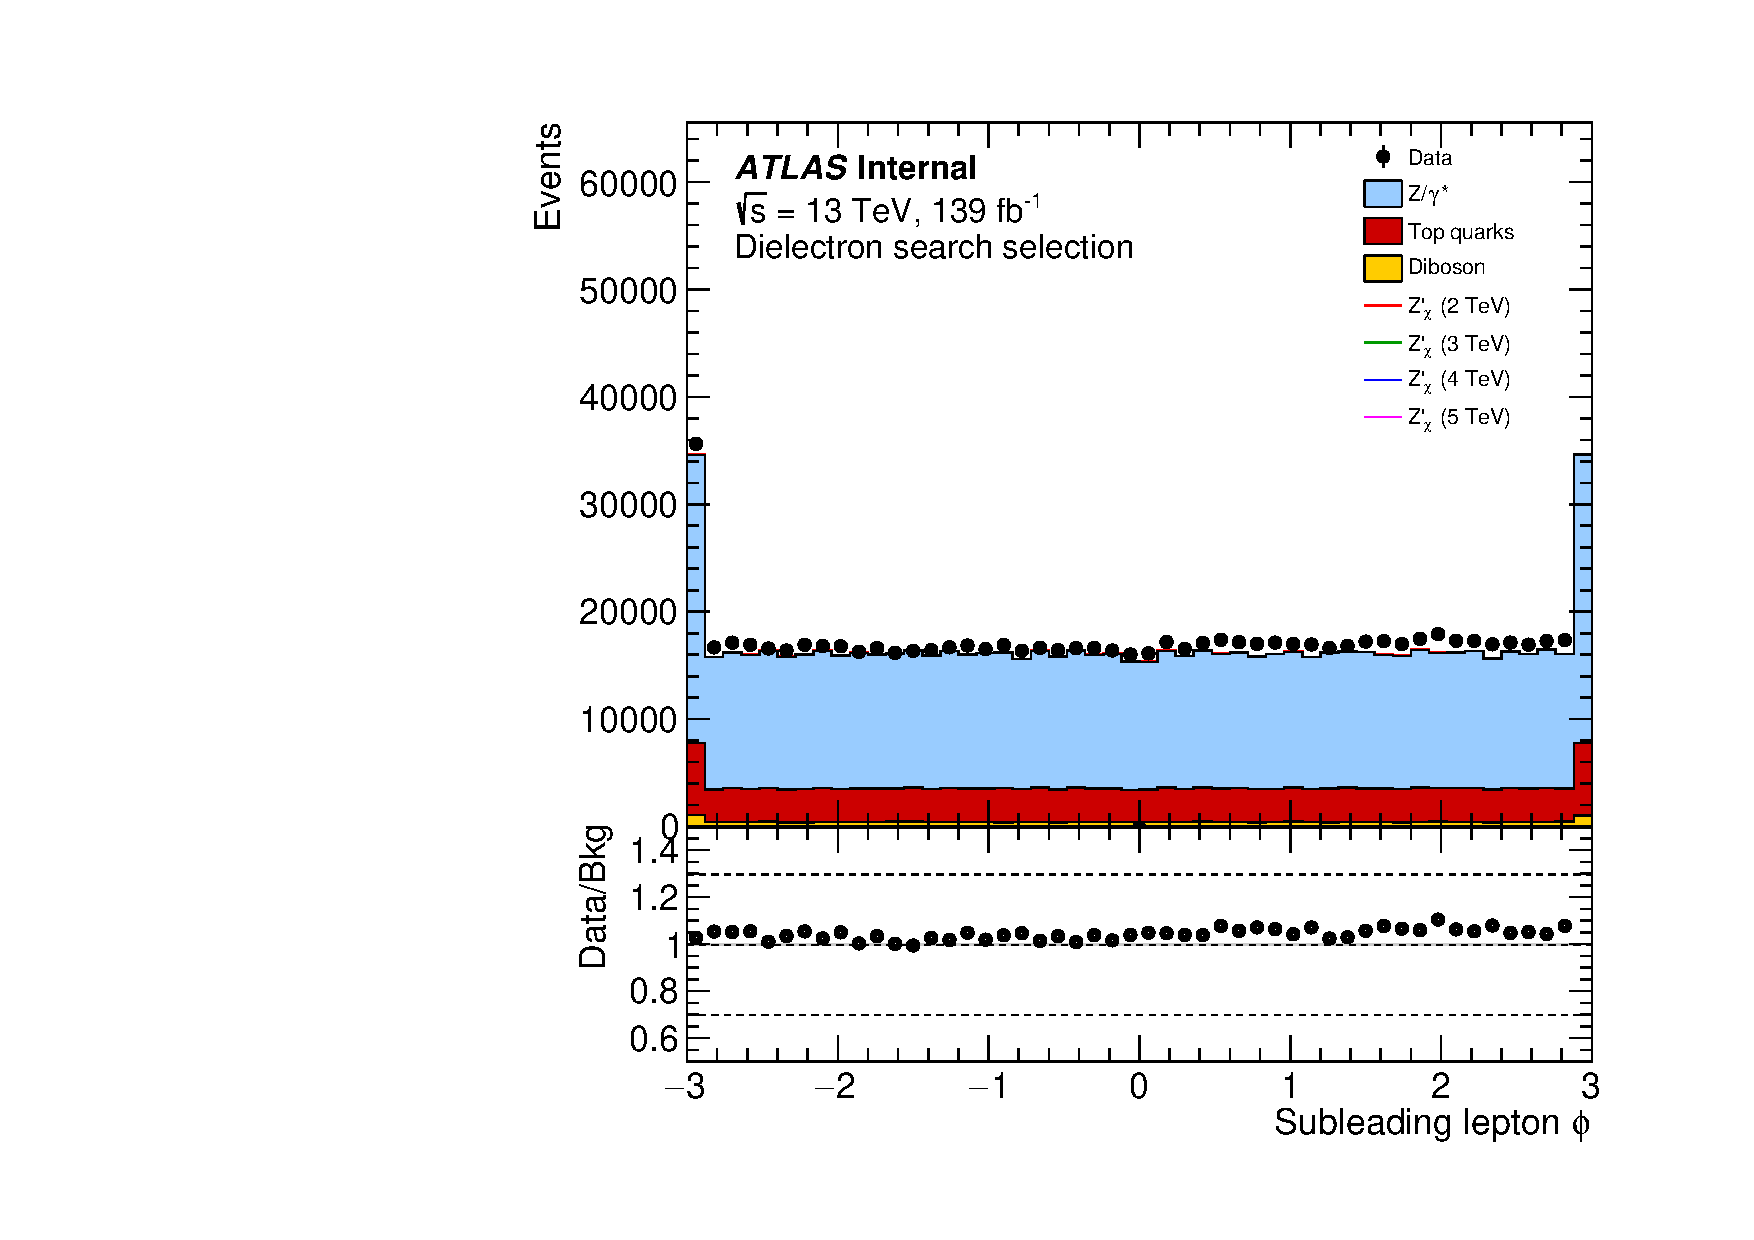
\includegraphics[width=1\textwidth]{figures/ci/dataMc/stacks_mc16e_2015-2018_ee_phi2.pdf}
    \subcaption{}
\end{minipage}
\caption{Kinematic distributions in the $ee$ channel. (a) $E_T^\text{miss}$, (b) dielectron \pt, leading electron $\phi$, and subleading electron $\phi$.}
\label{fig:}
\end{figure}
\clearpage
}

\afterpage{
\begin{figure}[h!]
\captionsetup[subfigure]{position=b}
\centering
\begin{minipage}[b]{.45\linewidth}
    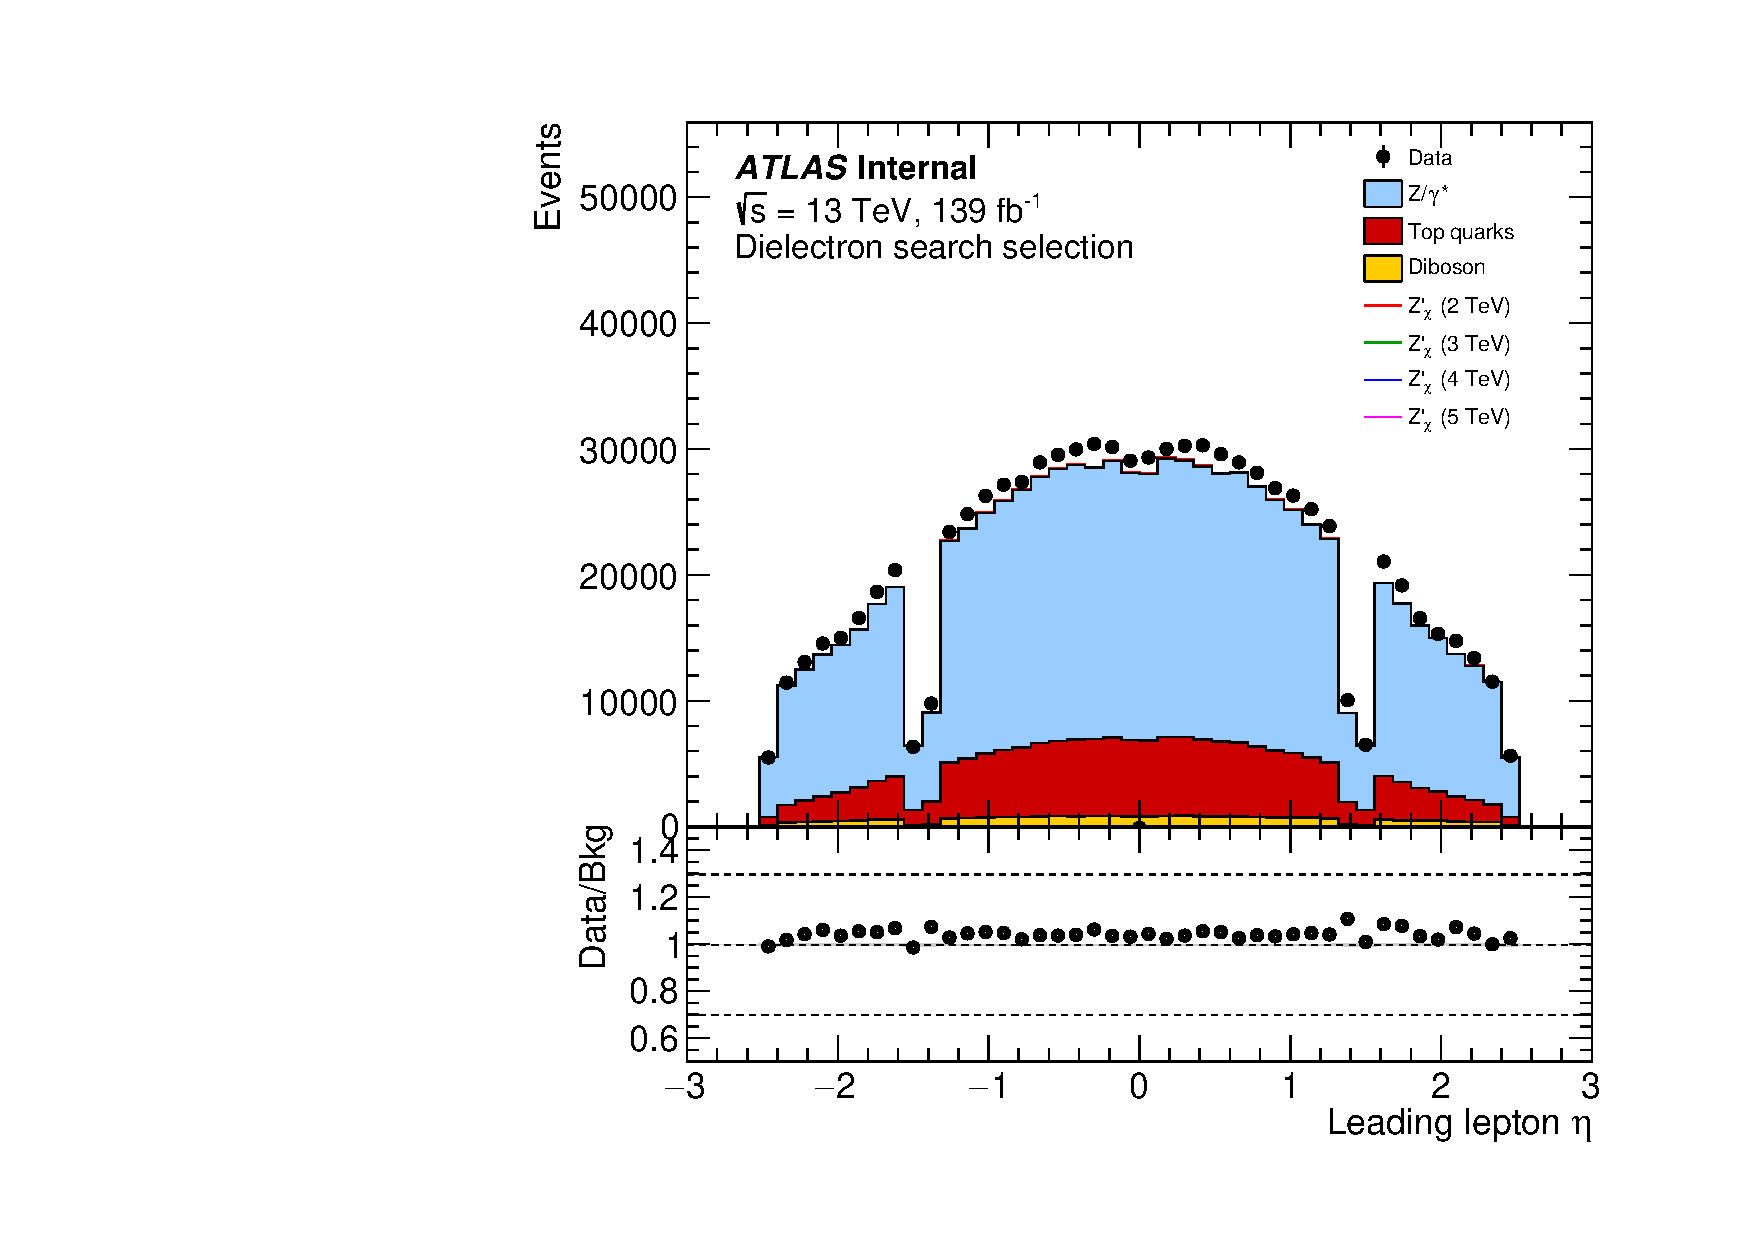
\includegraphics[width=1\textwidth]{figures/ci/dataMc/stacks_mc16e_2015-2018_ee_eta1.pdf}
    \subcaption{}
\end{minipage} 
\begin{minipage}[b]{.45\linewidth}
    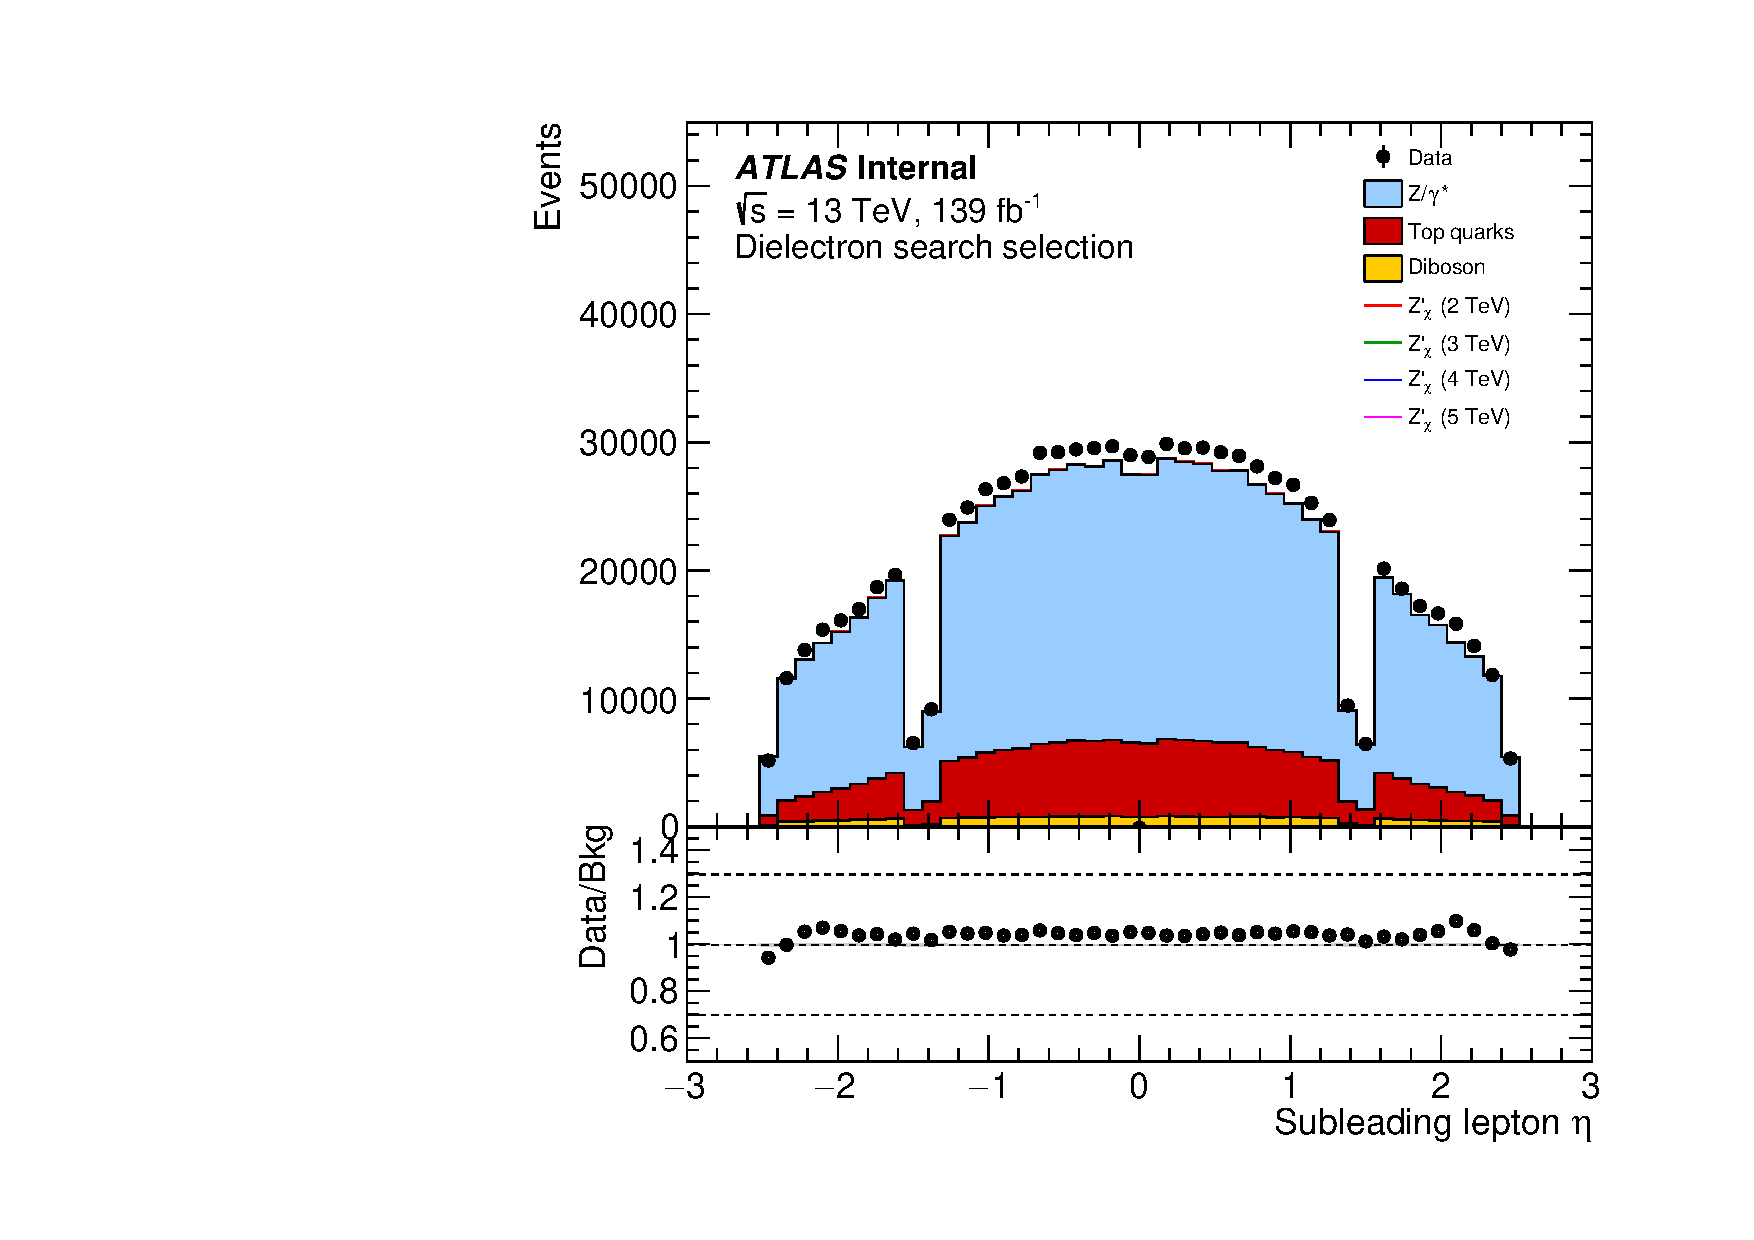
\includegraphics[width=1\textwidth]{figures/ci/dataMc/stacks_mc16e_2015-2018_ee_eta2.pdf}
    \subcaption{}
\end{minipage}\\
\begin{minipage}[b]{.45\linewidth}
    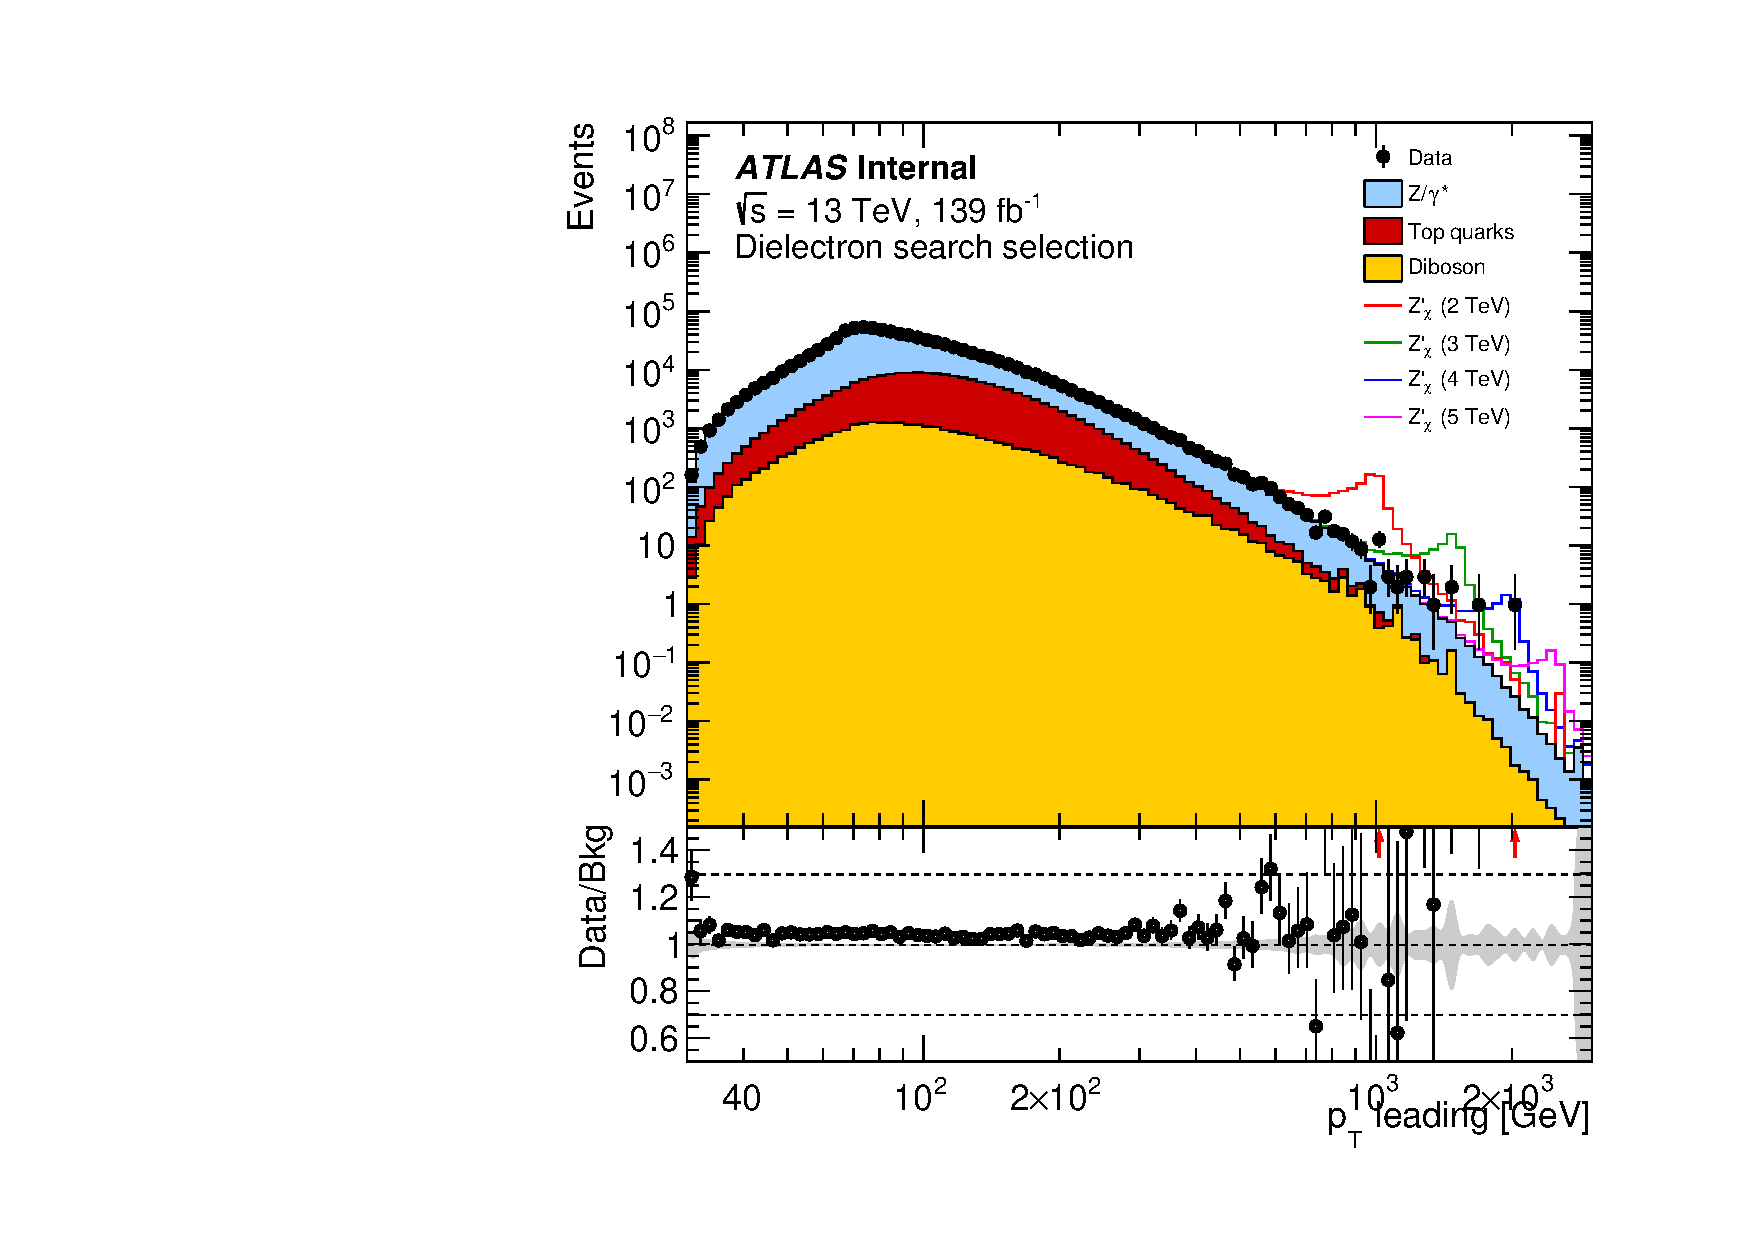
\includegraphics[width=1\textwidth]{figures/ci/dataMc/stacks_mc16e_2015-2018_ee_pt1_log100.pdf}
    \subcaption{}
\end{minipage}
\begin{minipage}[b]{.45\linewidth}
    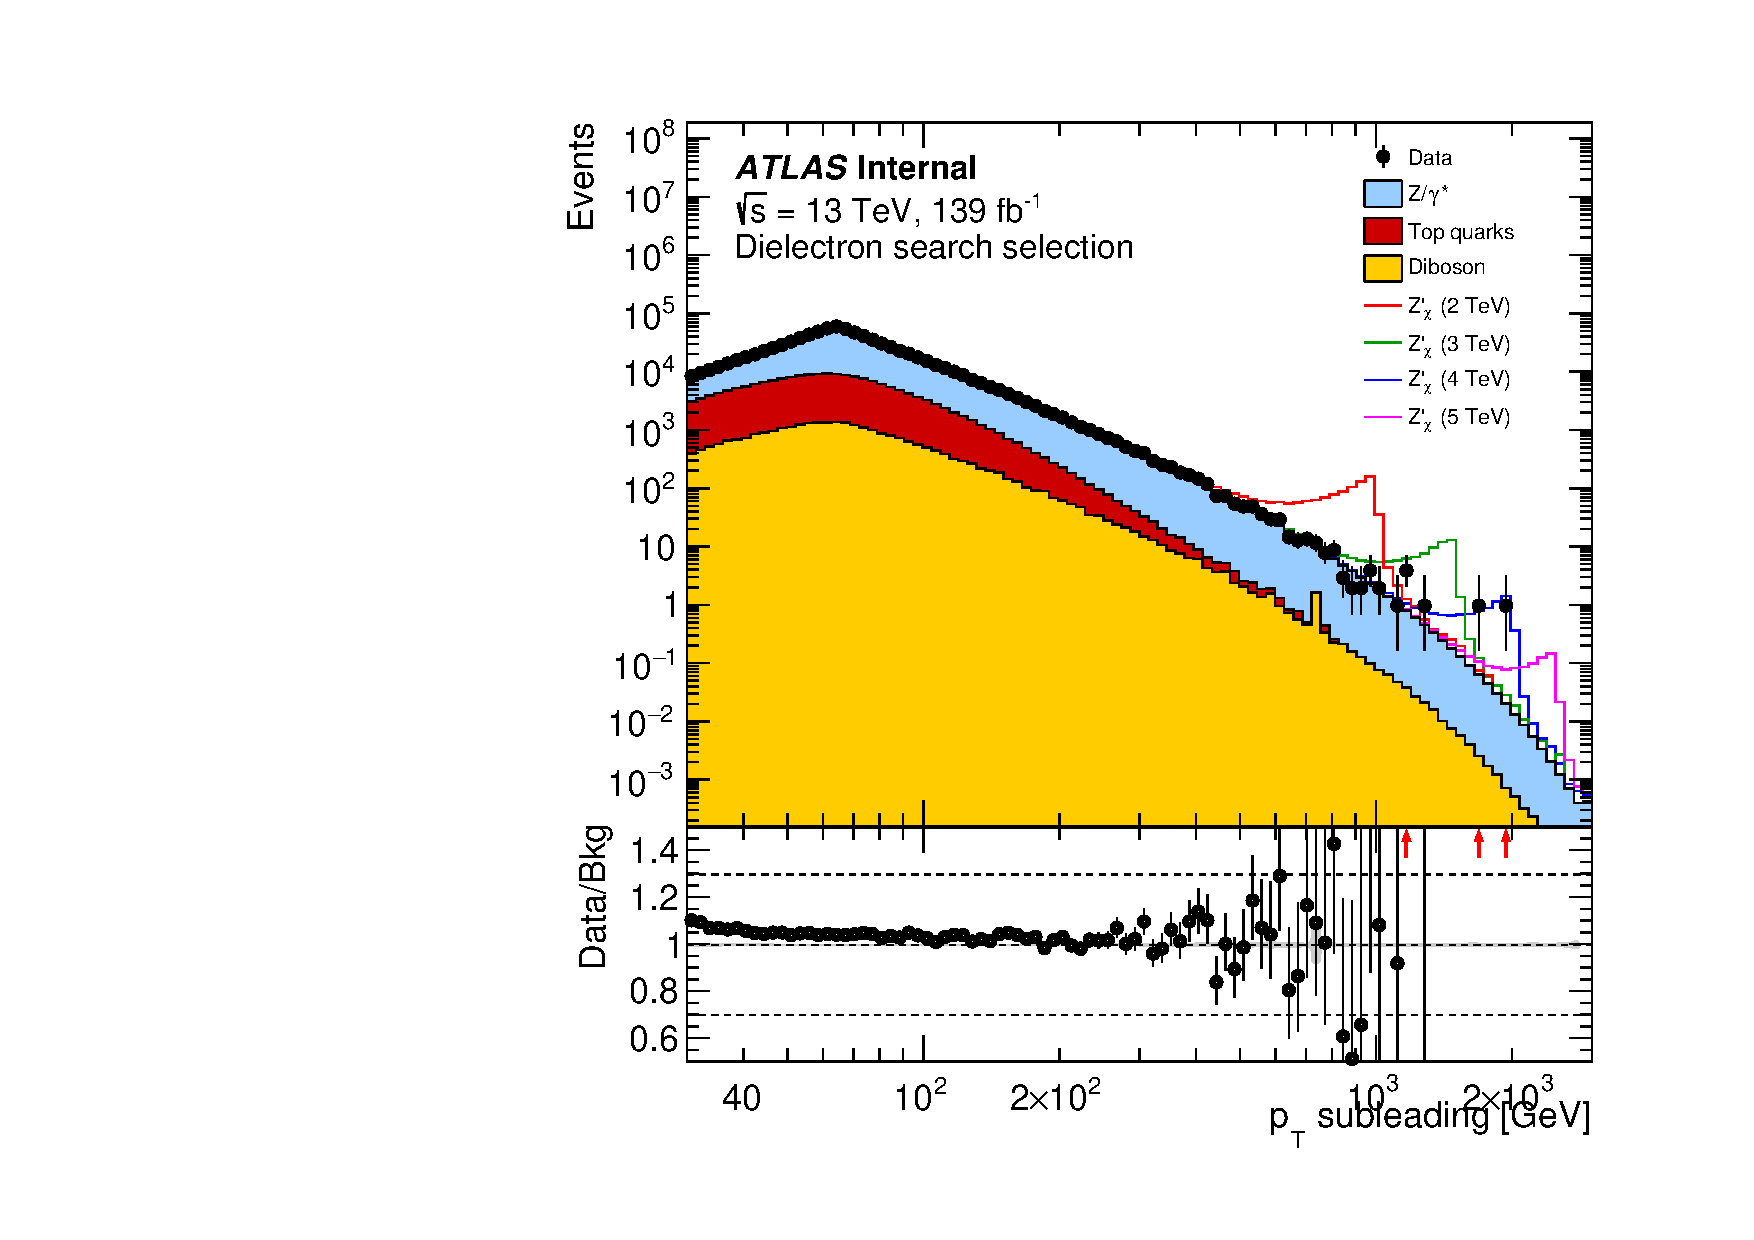
\includegraphics[width=1\textwidth]{figures/ci/dataMc/stacks_mc16e_2015-2018_ee_pt2_log100.pdf}
    \subcaption{}
\end{minipage}
\caption{Kinematic distributions in the $ee$ channel. (a) leading electron $\eta$, (b) subleading electron $\eta$, leading electron \pt, and subleading electron \pt.}
\label{fig:}
\end{figure}
\clearpage
}

\afterpage{
\begin{figure}[h!]
\captionsetup[subfigure]{position=b}
\centering
 \begin{minipage}[b]{.45\linewidth}
    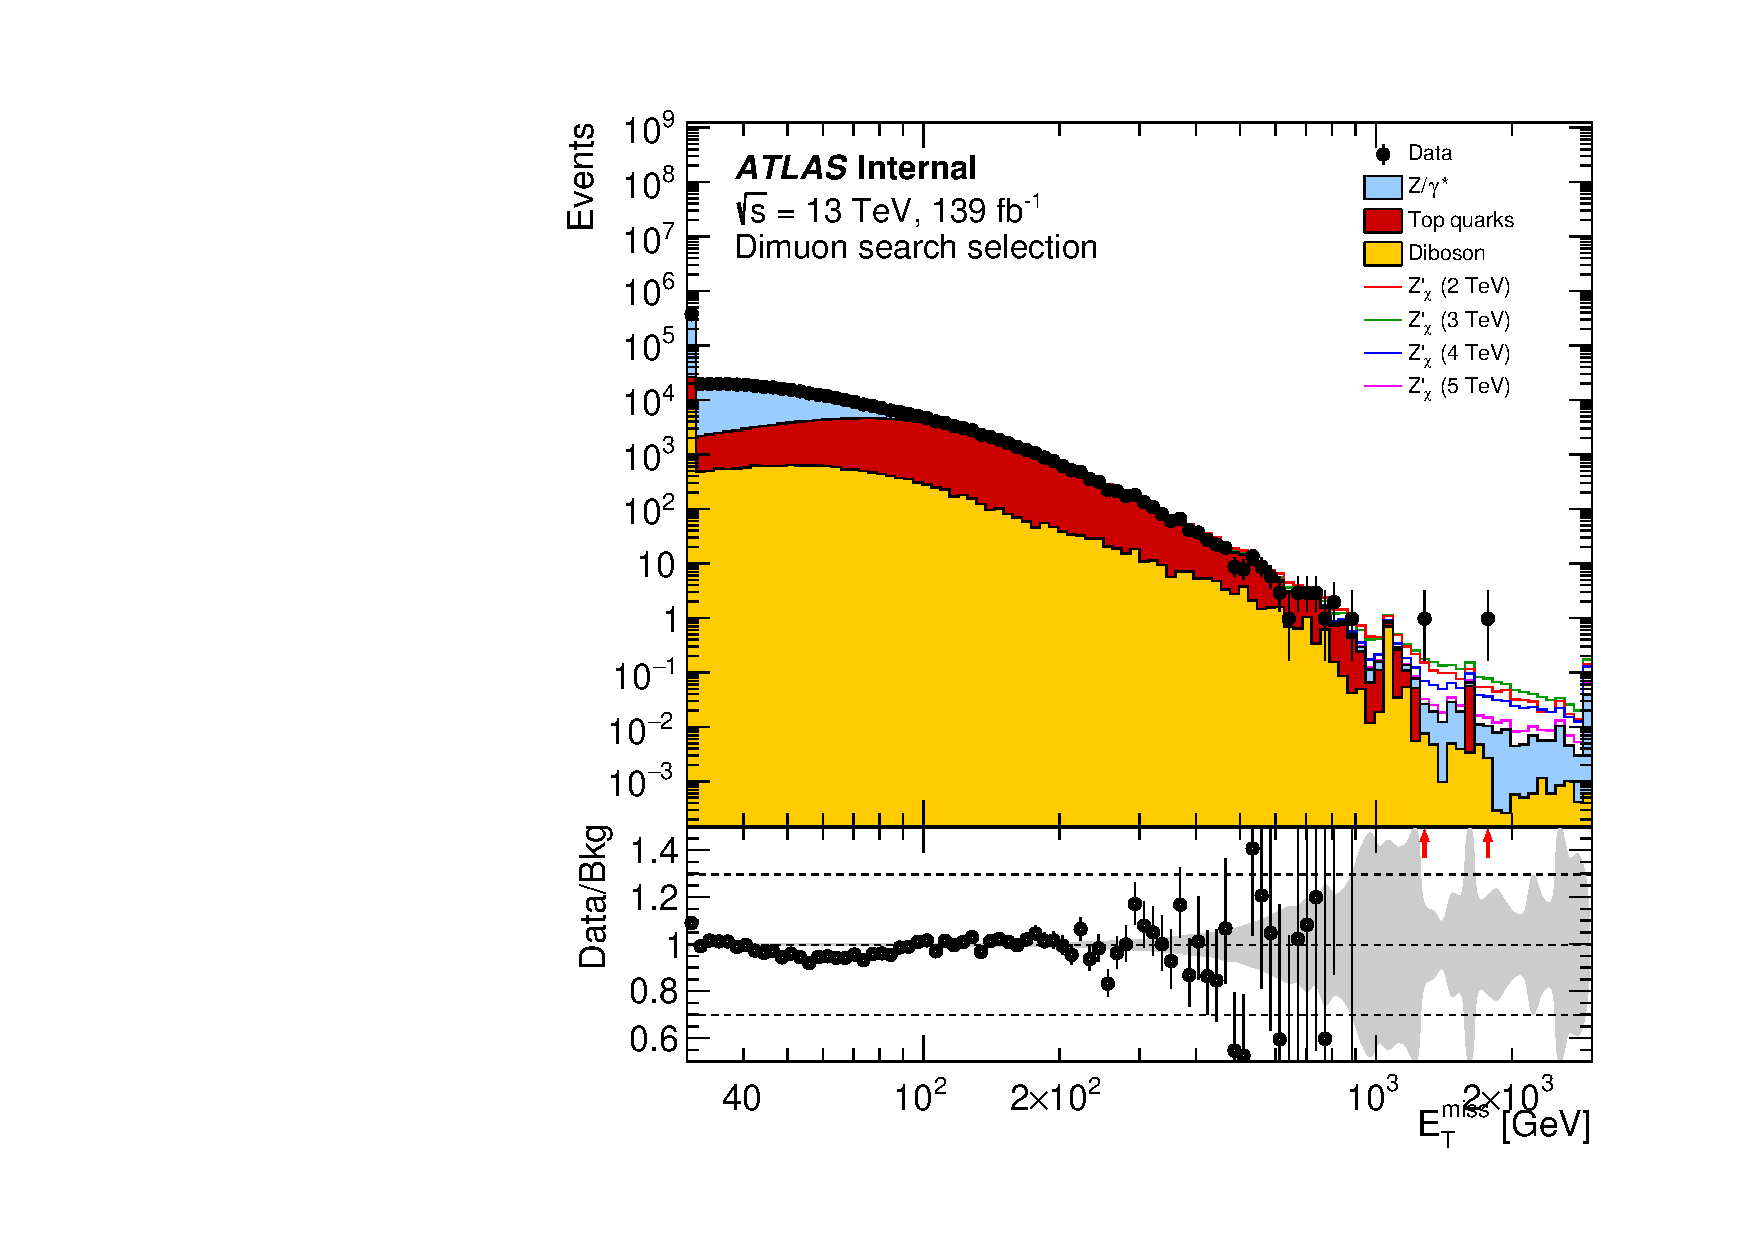
\includegraphics[width=1\textwidth]{figures/ci/dataMc/stacks_mc16e_2015-2018_uu_met_log100.pdf}
    \subcaption{}\label{fig:1a}
\end{minipage}
\begin{minipage}[b]{.45\linewidth}
    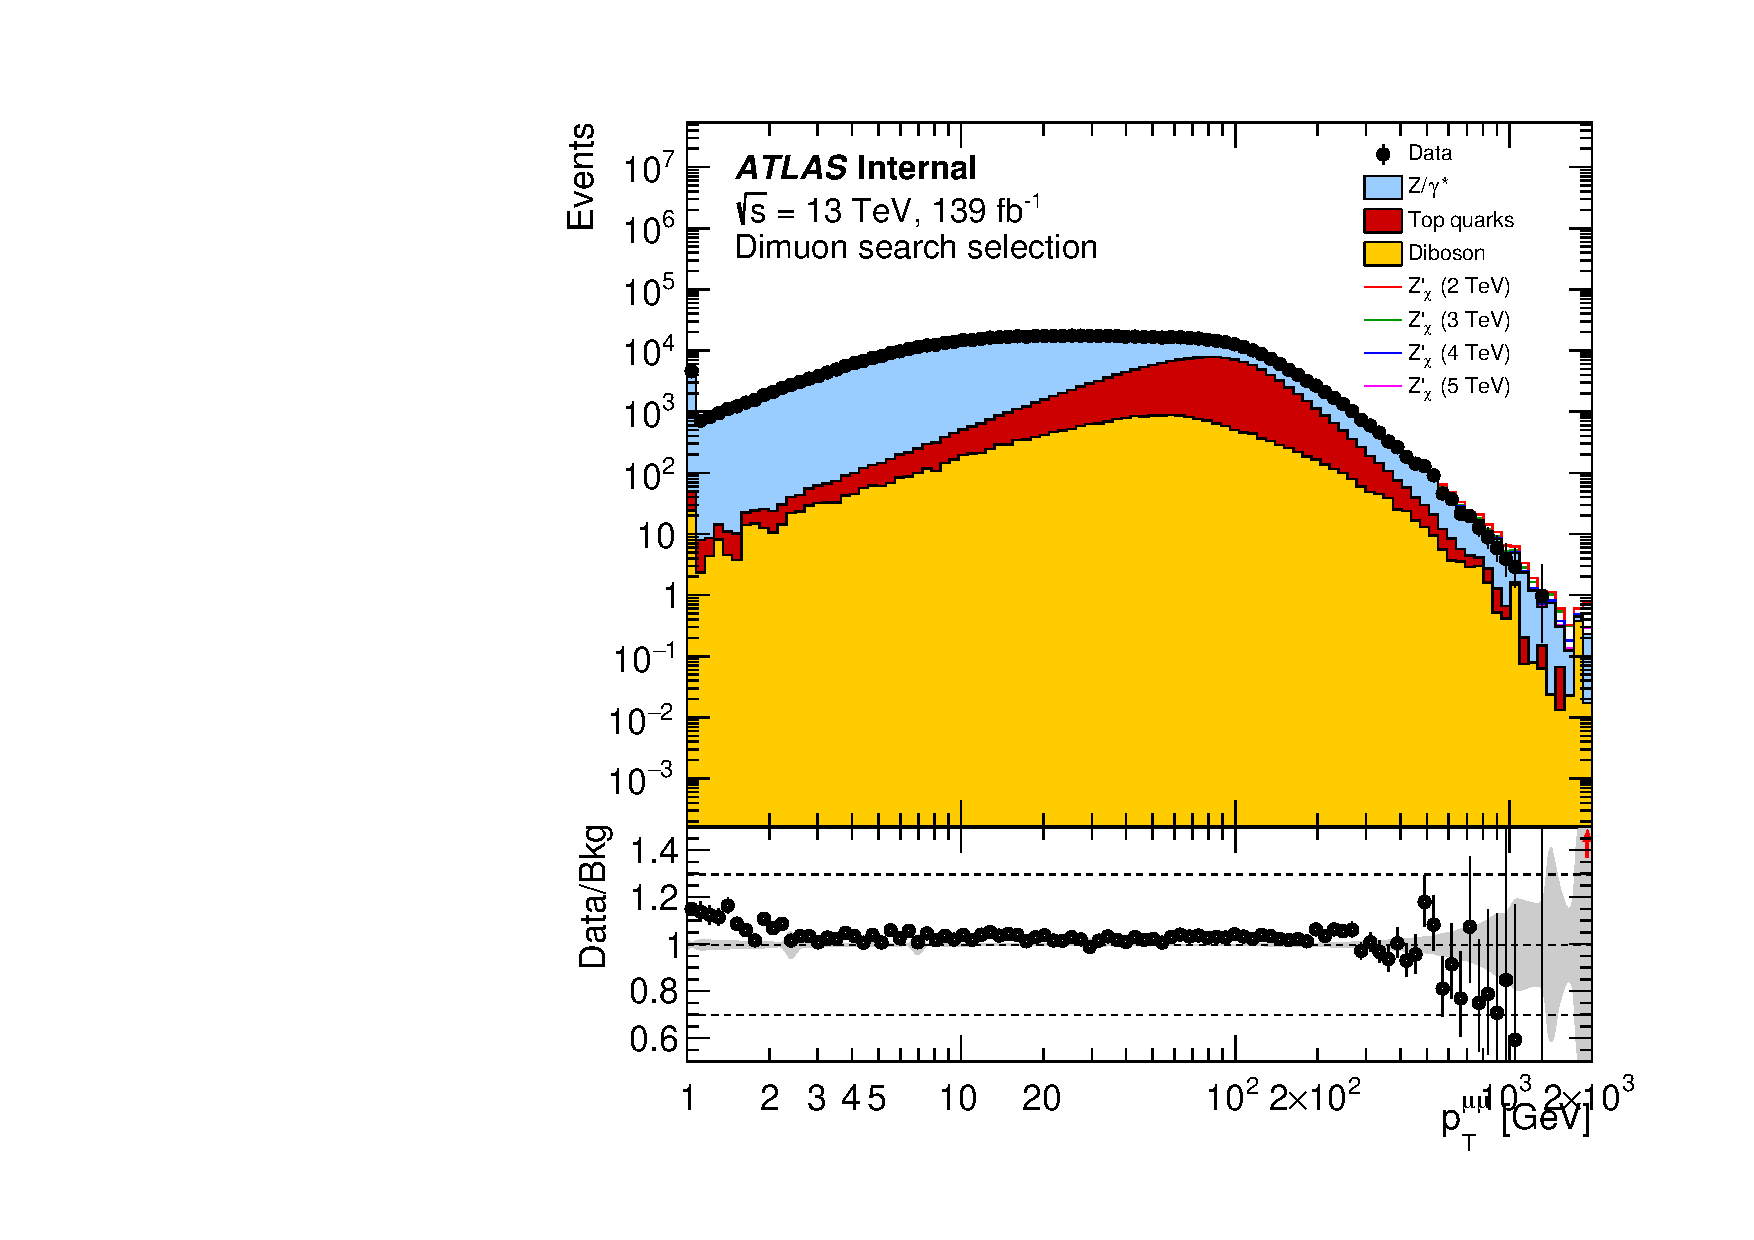
\includegraphics[width=1\textwidth]{figures/ci/dataMc/stacks_mc16e_2015-2018_uu_ptll_log100.pdf}
    \subcaption{}
\end{minipage} \\
\begin{minipage}[b]{.45\linewidth}
    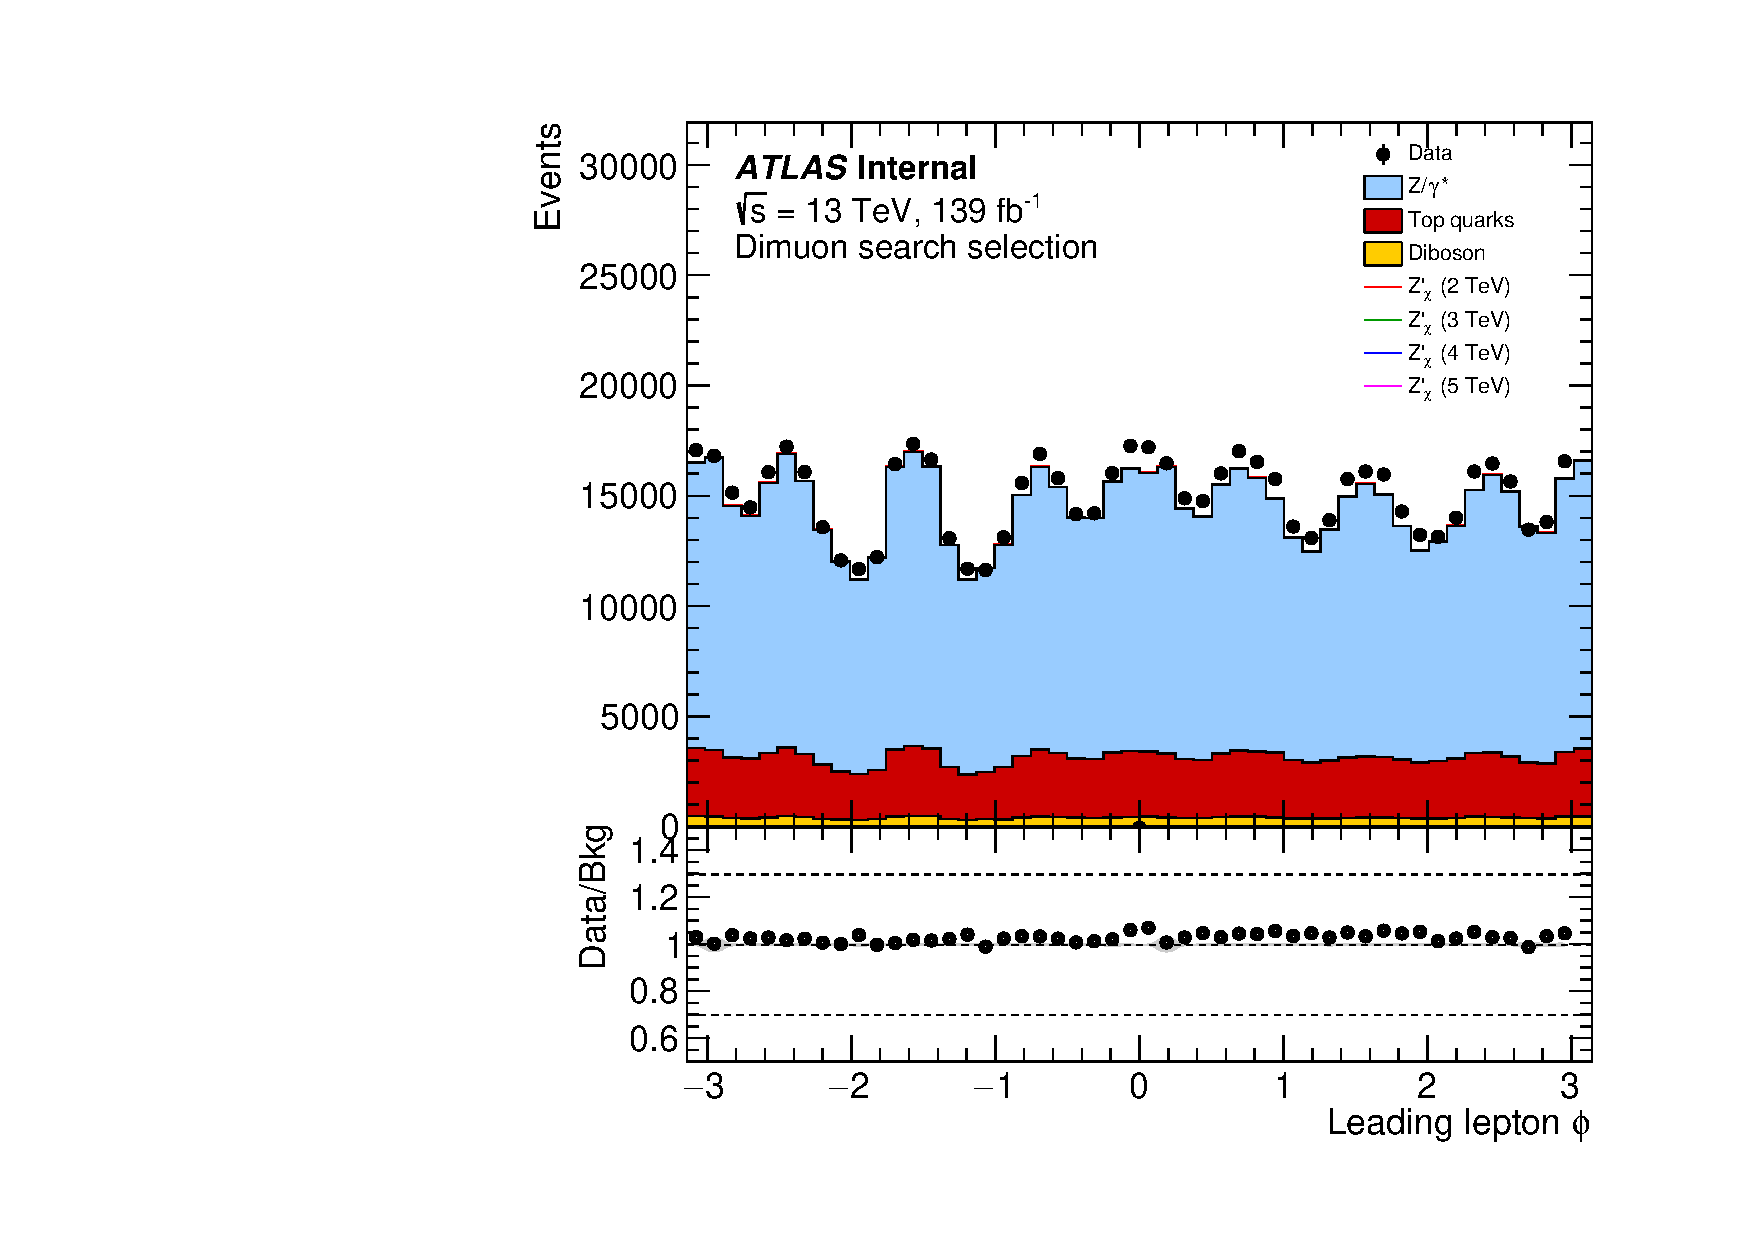
\includegraphics[width=1\textwidth]{figures/ci/dataMc/stacks_mc16e_2015-2018_uu_phi1.pdf}
    \subcaption{}
\end{minipage}
\begin{minipage}[b]{.45\linewidth}
    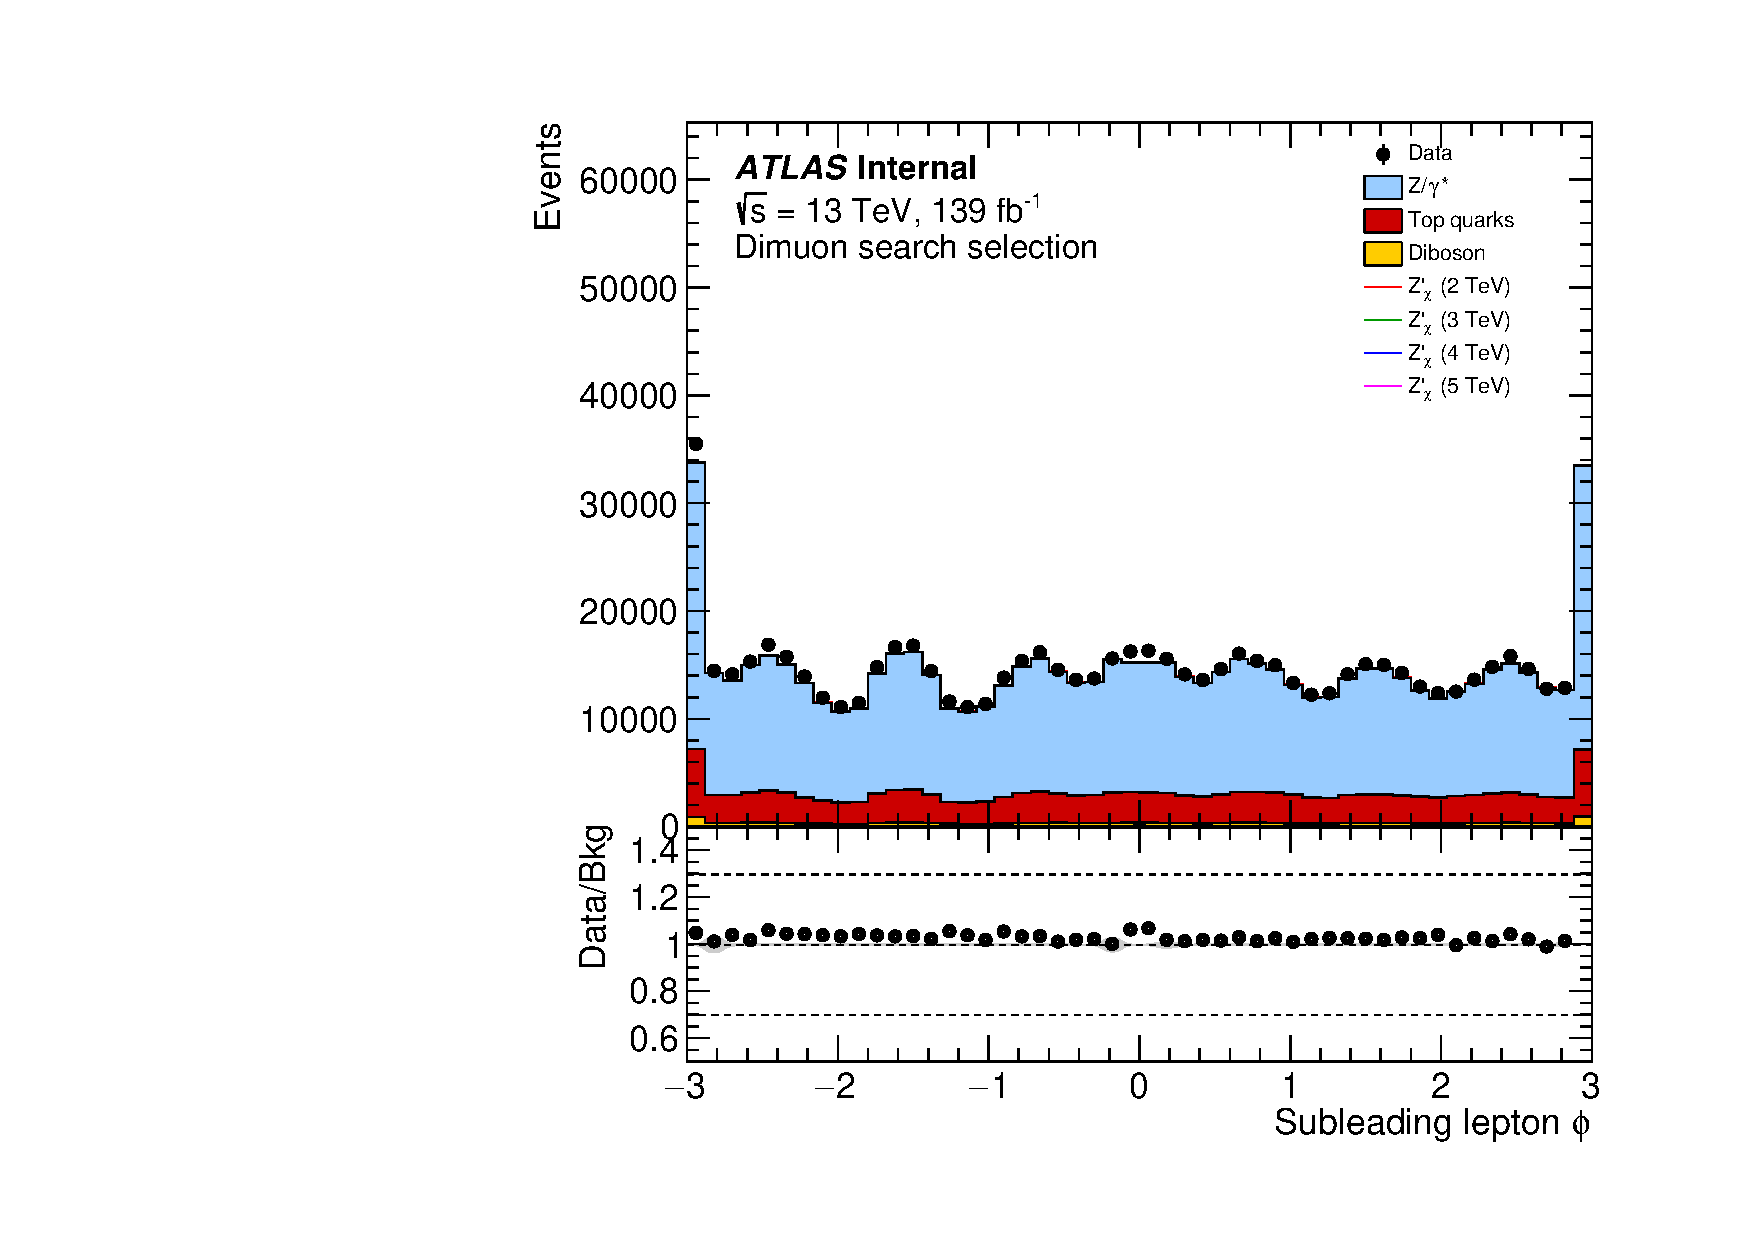
\includegraphics[width=1\textwidth]{figures/ci/dataMc/stacks_mc16e_2015-2018_uu_phi2.pdf}
    \subcaption{}
\end{minipage}
\caption{Kinematic distributions in the $\mu\mu$ channel. (a) $E_T^\text{miss}$, (b) dielectron \pt, leading muon $\phi$, and subleading muon $\phi$.}
\label{fig:}
\end{figure}
\clearpage
}

\afterpage{
\begin{figure}[h!]
\captionsetup[subfigure]{position=b}
\centering
\begin{minipage}[b]{.45\linewidth}
    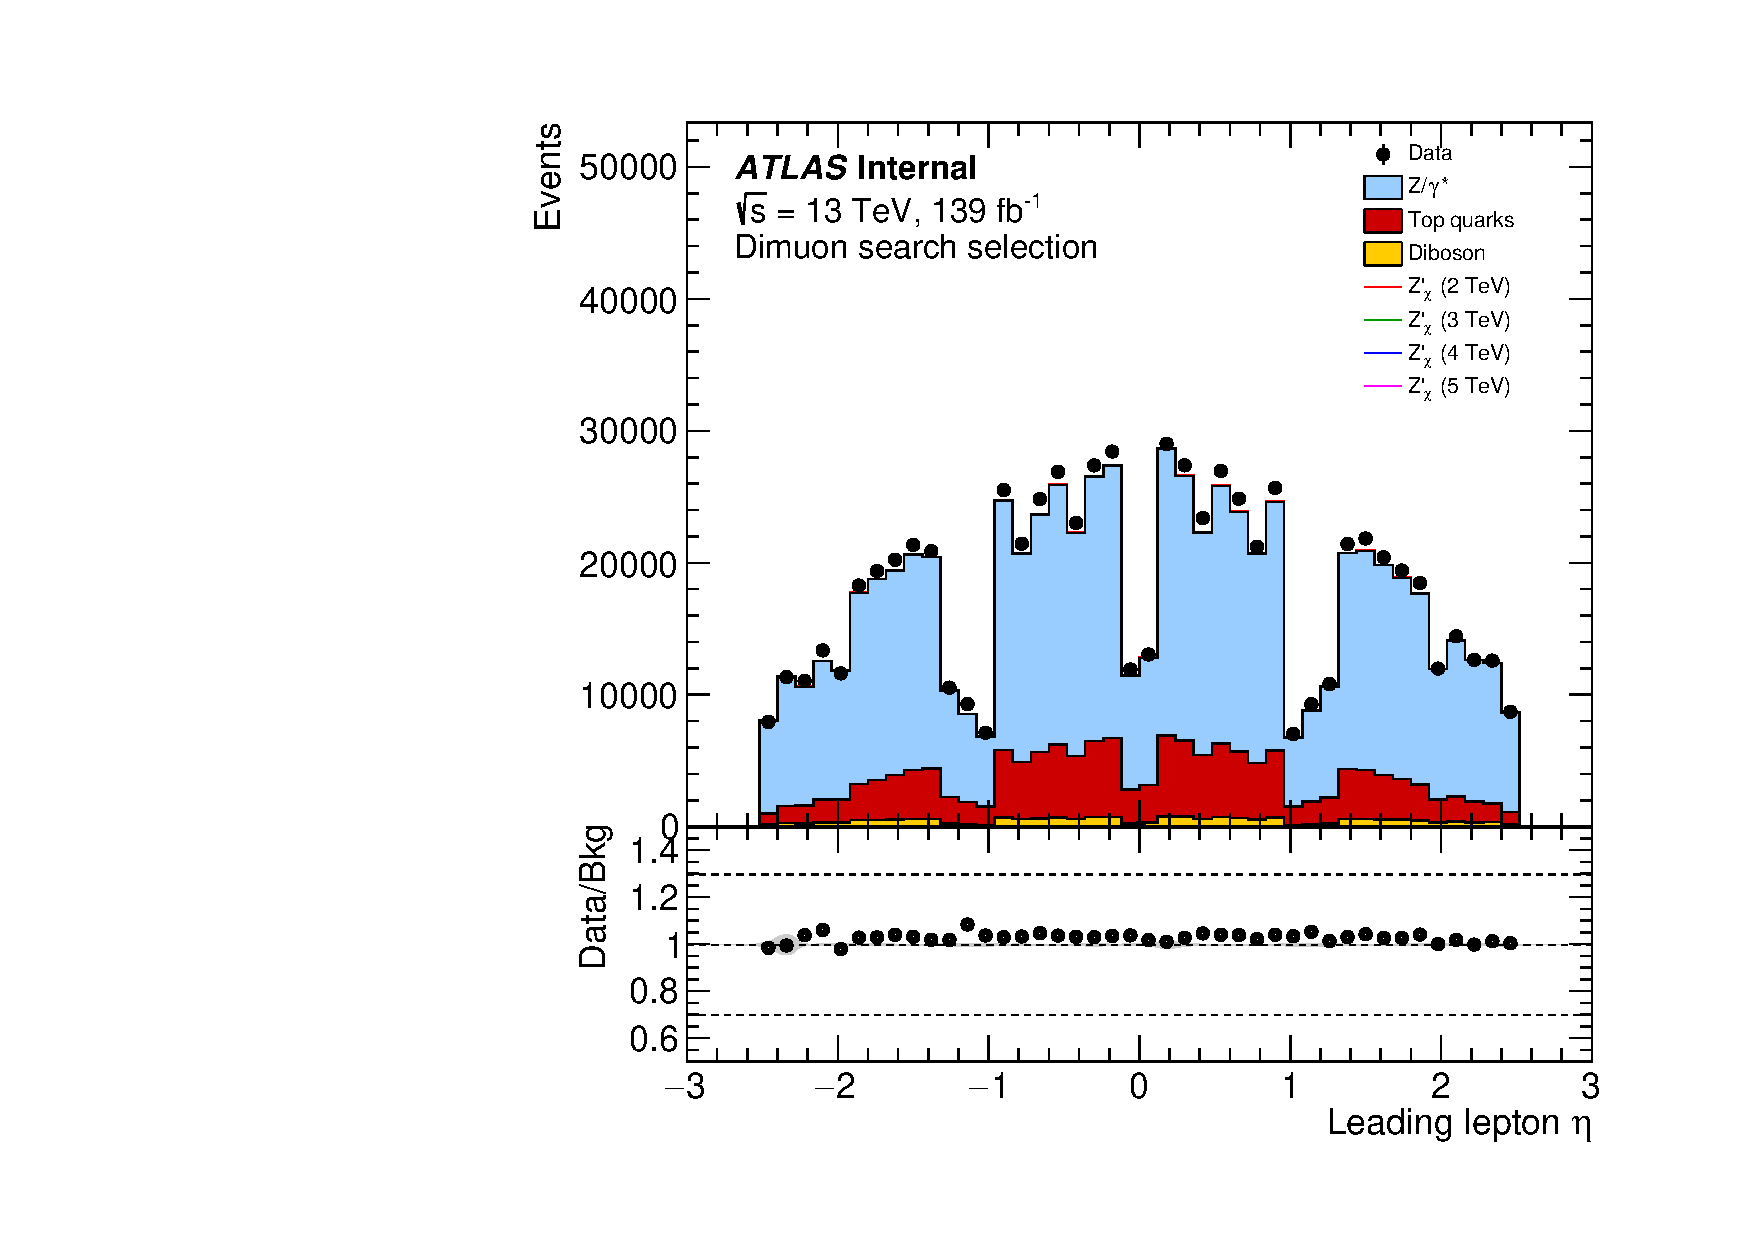
\includegraphics[width=1\textwidth]{figures/ci/dataMc/stacks_mc16e_2015-2018_uu_eta1.pdf}
    \subcaption{}
\end{minipage} 
\begin{minipage}[b]{.45\linewidth}
    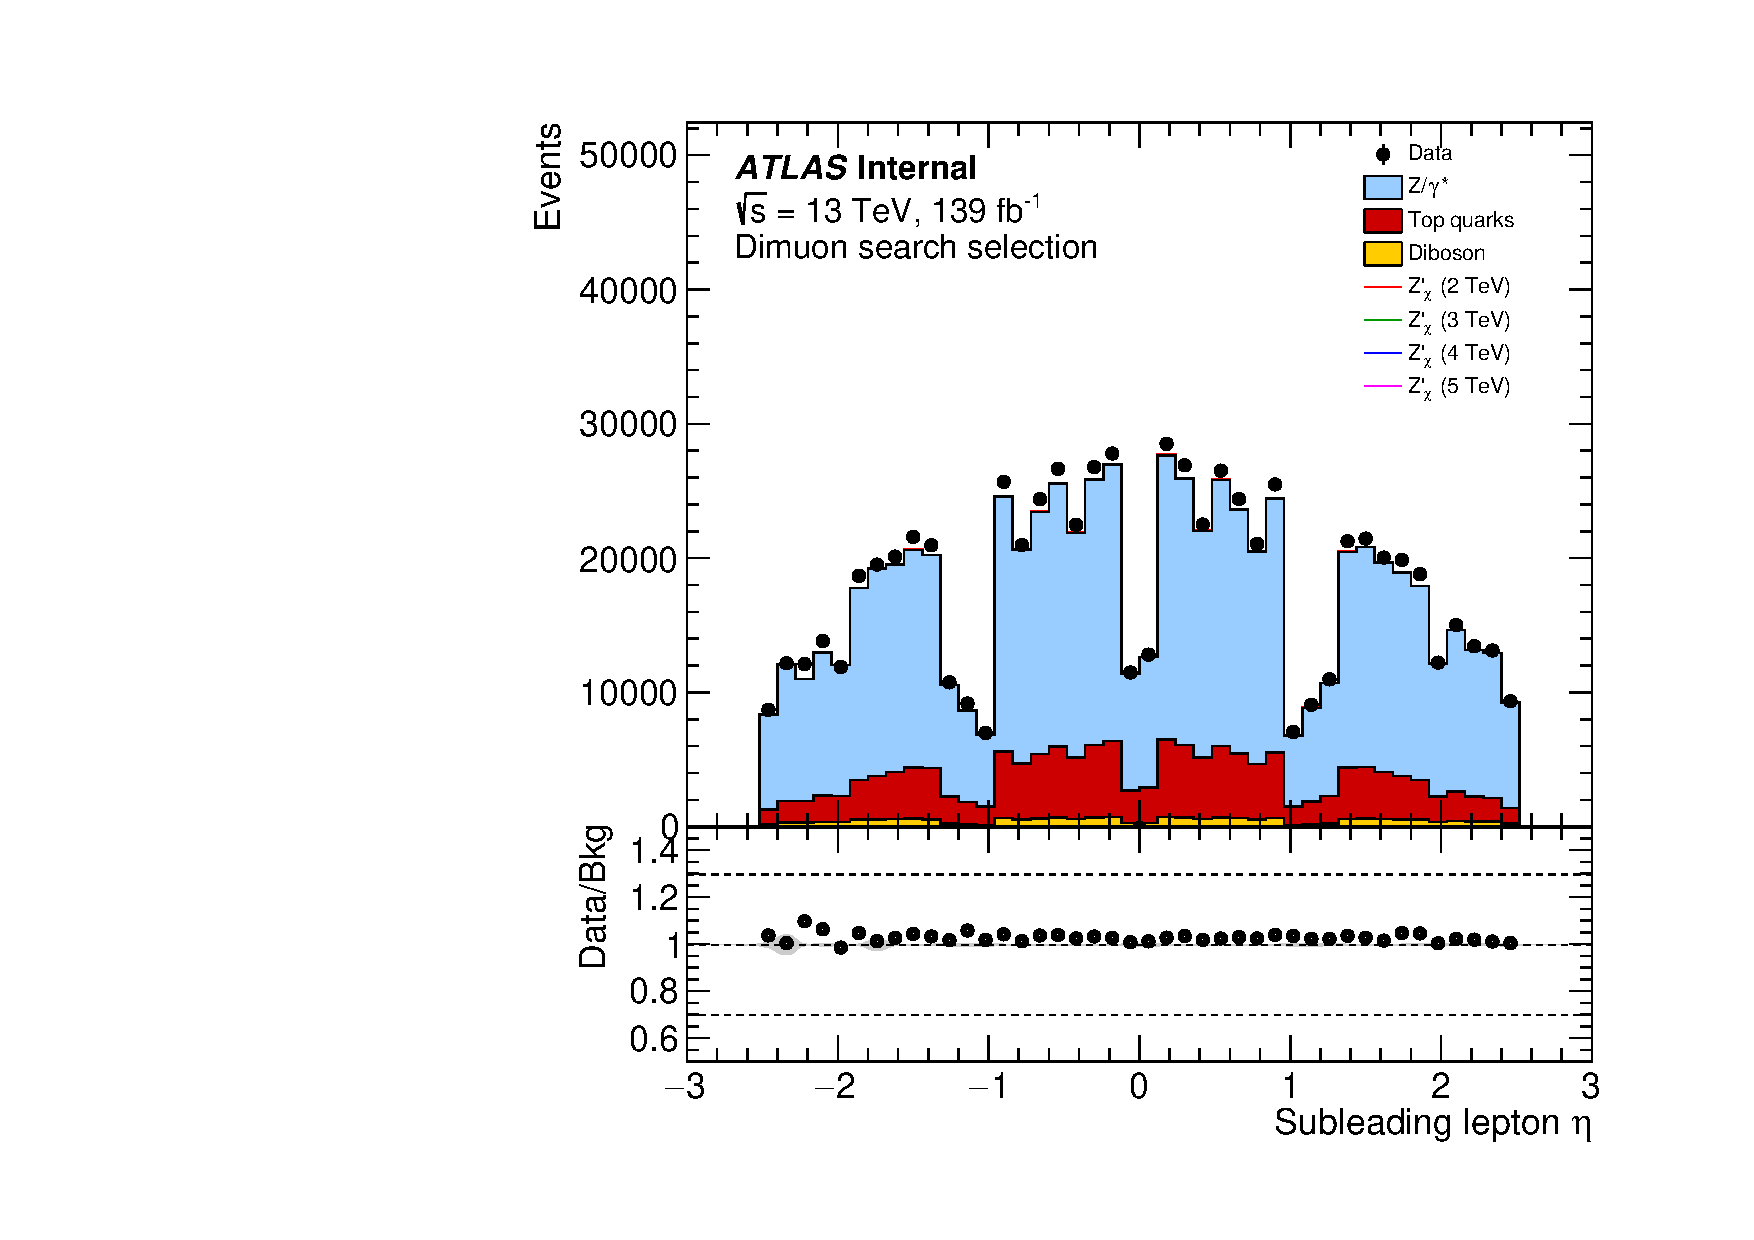
\includegraphics[width=1\textwidth]{figures/ci/dataMc/stacks_mc16e_2015-2018_uu_eta2.pdf}
    \subcaption{}
\end{minipage}\\
\begin{minipage}[b]{.45\linewidth}
    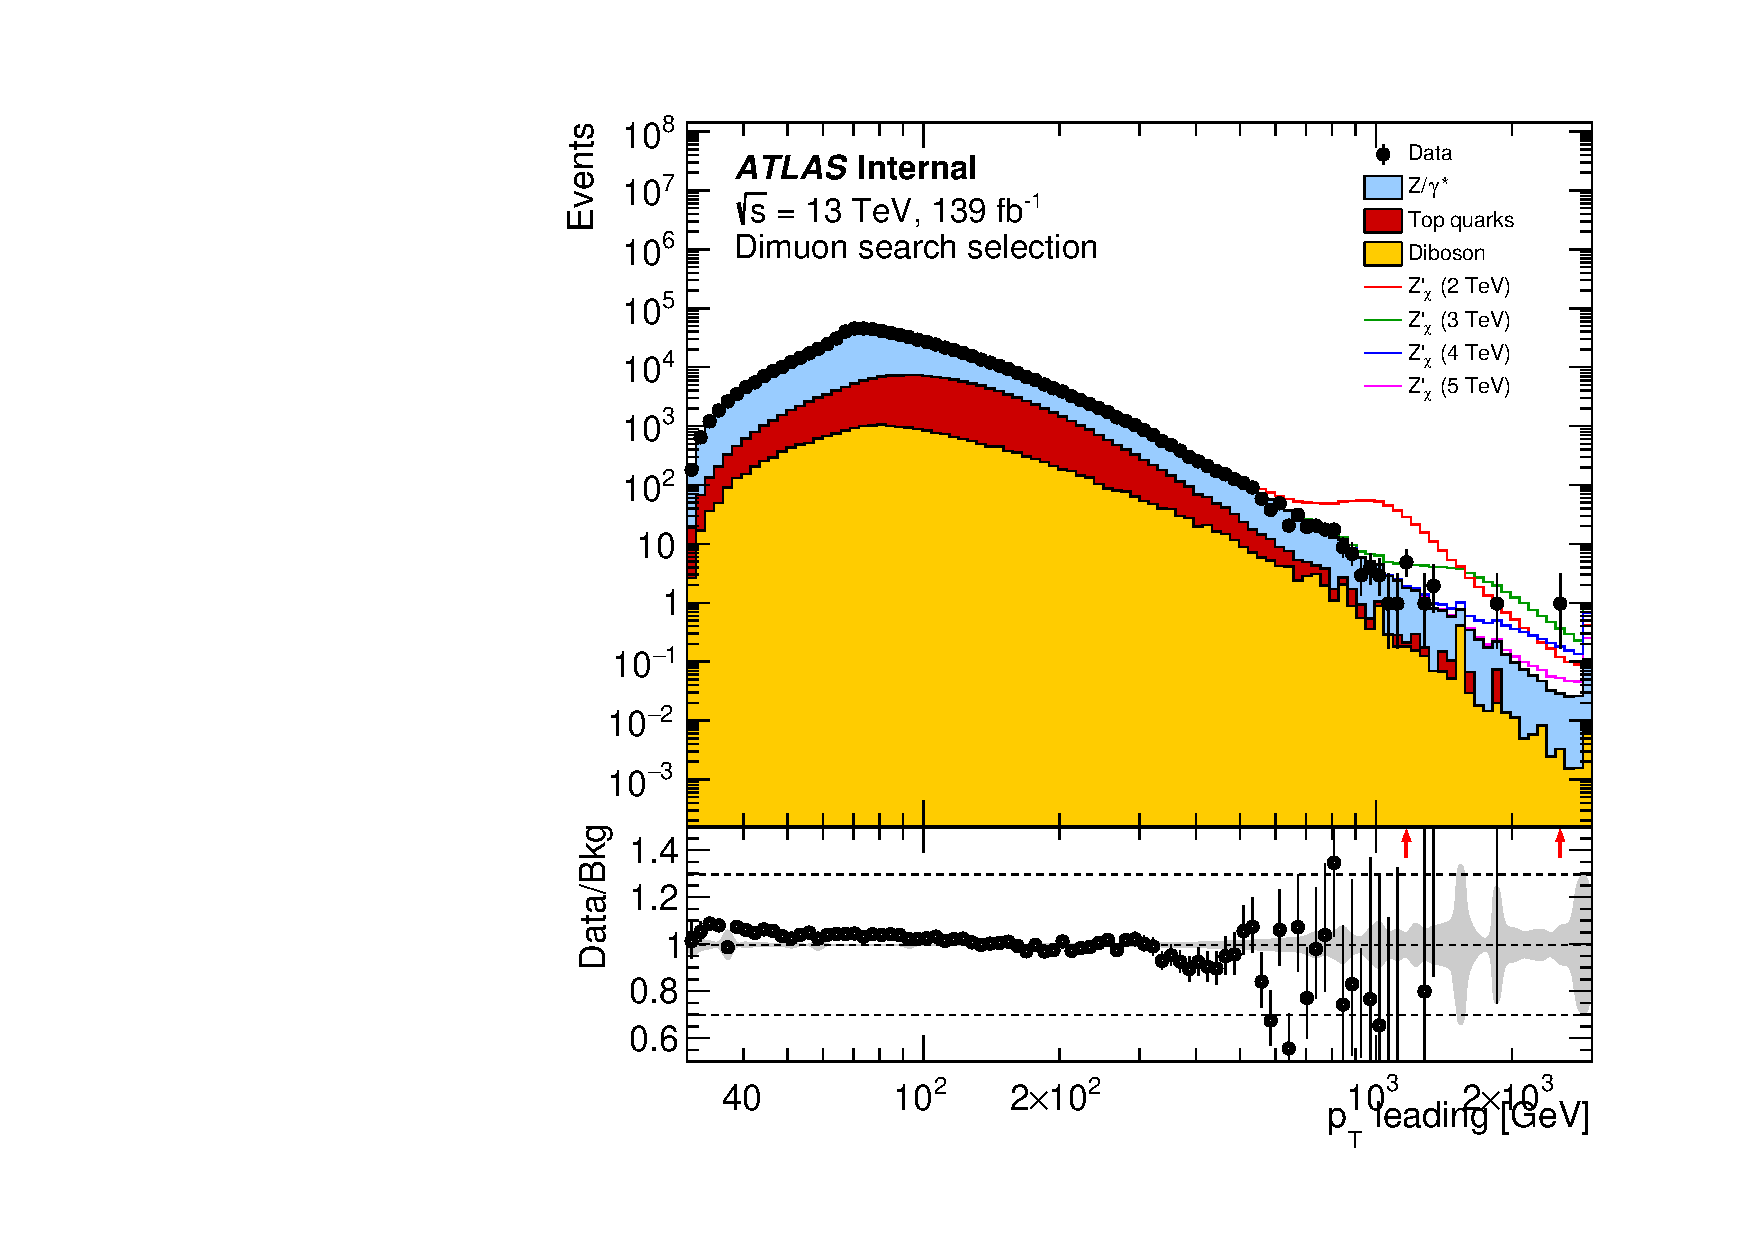
\includegraphics[width=1\textwidth]{figures/ci/dataMc/stacks_mc16e_2015-2018_uu_pt1_log100.pdf}
    \subcaption{}
\end{minipage}
\begin{minipage}[b]{.45\linewidth}
    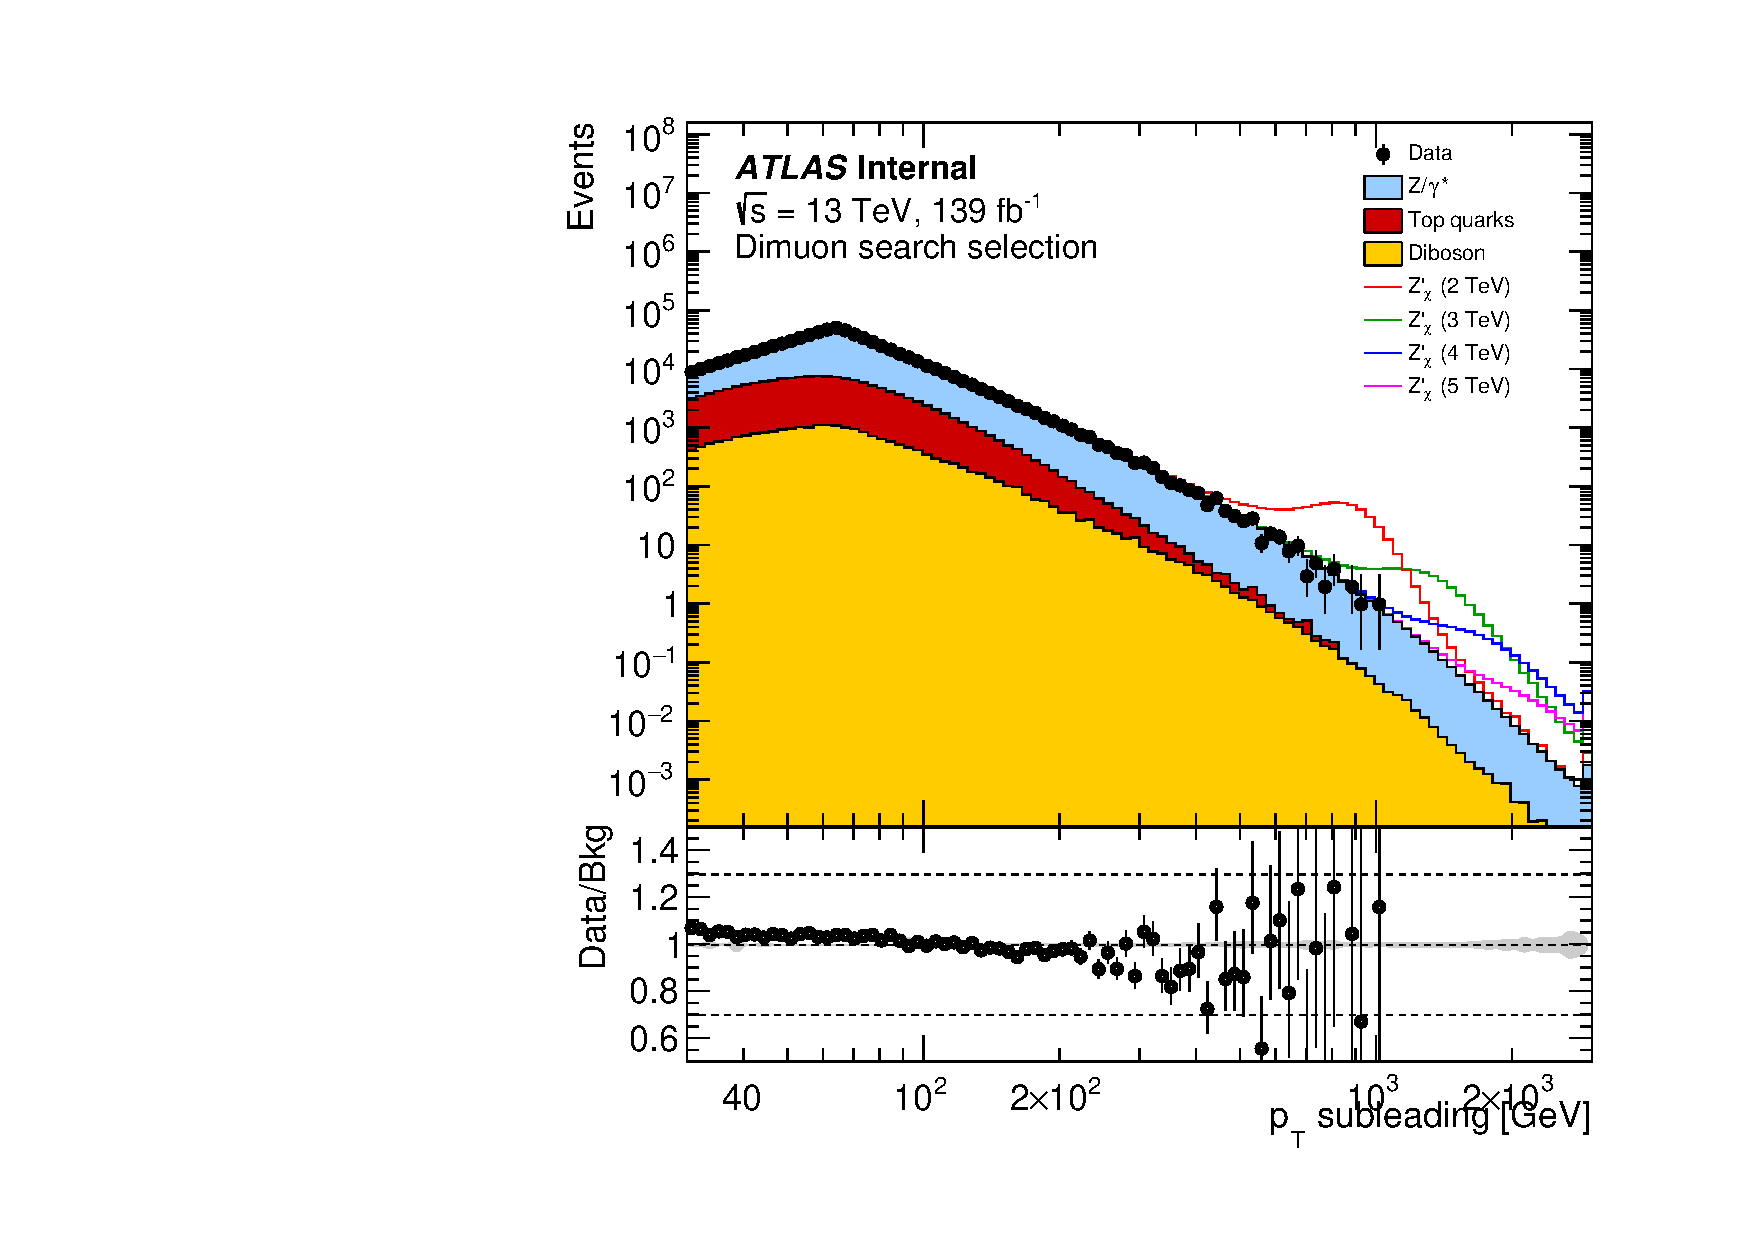
\includegraphics[width=1\textwidth]{figures/ci/dataMc/stacks_mc16e_2015-2018_uu_pt2_log100.pdf}
    \subcaption{}
\end{minipage}
\caption{Kinematic distributions in the $\mu\mu$ channel. (a) leading muon $\eta$, (b) subleading muon $\eta$, leading muon \pt, and subleading electron \pt.}
\label{fig:}
\end{figure}
\clearpage
}

\clearpage

\section{Background Modeling}\label{sec:ciBkg}

An expectation of the number of events under the background-only hypothesis is needed for each of the four signal regions.
This raises the question of what exactly is meant by \emph{background}.
In the full mass range, the observed data are considered to have been produced according to some PDF.
If the PDF does not contribute from a signal-like production mechanism, then this is a background-PDF.
This is emphatically not the same thing as the physical truth-PDF that has generated the collected data.
The background-only hypothesis predicts that the event yield in each signal region equals the yield predicted by the background-PDF, normalized to match the integrated luminosity.
Of course, this background-PDF is not explicitly known, and therefore a methodology for estimating it's predicted yield is needed.
This section describes how this is done using an estimate in the CR.

This search uses a functional form fit to the shape of the data in a low mass control region and extrapolated into the high mass signal region, where it is integrated.
In principle, any functional form is acceptable, as long as the uncertainties on the background estimate in the SR are properly measured.
In practice, to produce competitive results, it is necessary to select a functional form that well models the underlying distribution that has generated the background component of the data.

The functional form was chosen from an extensive list of candidates, drawn from similar studies, for its stability during extrapolations and the ability to model the simulated background. Here, stability refers to the function not to tend to behave nonphysically.
The procedure to determine the functional form of the background is as follows.
The smooth functional form used to model the background is chosen from about 50 candidate functions.
Each function is fit to the dilepton mass background template, consisting of the sum of all the simulated background contributions, in a variety of CRs, and extrapolated to the respective SRs.
The data and simulation are both fit using a binned-likelihood maximization with a bin width of 1~GeV.
The distribution of the pulls, defined as (fit--simulation)/fit for each bin, is obtained for each potential configuration of CR and SR.
A function that results in pulls below three across all the ranges considered (CRs and SRs) is marked as acceptable.
This requirement is particularly important in the SRs to veto functions that exhibit unphysical behavior at the tail.
Additionally, it is important to ensure a good description of the simulated background template in the CRs.
Out of about 50 initial functions, five are found to satisfy this requirement equally well.
The residual miss-modeling by the selected function is measured later and taken as an uncertainty.
The functions that were found to best satisfy these criteria are given in Equations \ref{eqn:ciBkgEe} and \ref{eqn:ciBkgMm} for $ee$ and $\mu\mu$ channels respectively.
\begin{equation}\begin{split} \label{eqn:ciBkgEe}
f_\textrm{b}(\mee) &= f_{\mathrm{BW},Z}(\mee) \cdot \left(1 - x\right)^{b} \cdot x^{\sum_{i=0}^3 p_i\log(x)^i} \\
\end{split}\end{equation} 
\begin{equation}\begin{split}\label{eqn:ciBkgMm}
f_\textrm{b}(\mee) &= f_{\mathrm{BW},Z}(\mee) \cdot \left(1 - x^{1/3}\right)^{b} \cdot x^{\sum_{i=0}^3 p_i\log(x)^i} \\
\end{split}\end{equation} 
where $x = m_{\ell\ell}/\sqrt{s}$.
The first term, $f_{\mathrm{BW},Z}(m_{\ell\ell})$, is a non-relativistic Breit--Wigner function with $m_Z = 91.1876$~GeV and $\Gamma_Z = 2.4952$~GeV.
This primarily dictates the function shape in the low-mass regime of the control region.
The second term, $(1-x^{c})^{b}$, shapes the high-mass behavior of the function by ensuring that the background shape evaluates to zero at $x\to 1$.
The parameter $b$ is fixed to values obtained from fits to the simulated background.
In the third term, the parameters $p_i$ with $i=0,..,3$ are left free in the fits.
The function $f_\textrm{b}(m_{\ell\ell})$ is treated as a probability density function in the fits performed in the CR.
This function is then normalized in the CR to $N_\textrm{CR}$, the number of events in the CR in data (or simulation where applicable), where it is assumed that the CR is completely dominated by background events.

The fits are performed using a binned likelihood maximization using the MINUIT algorithm \cite{minuit}.
The functional forms of Equations \ref{eqn:ciBkgEe} and \ref{eqn:ciBkgMm} are fit to a \emph{template}, which may is a histogram filled by either data or simulated data.
In this process, the total log-likelihood of the template is calculated as the sum of the log-likelihood of each template bin to have been generated by the functional form.
Then, each of the flexible parameters of the functional forms is adjusted with MINUIT until the total log-likelihood has reached a maximum.
The functional form with these parameter fitted values is the function with the highest likelihood to generate the observed data.

% Definitions of function vs ''background model''
It is worth explicating some nomenclature. 
The normalized and fitted functions of Equations \ref{eqn:ciBkgEe} and \ref{eqn:ciBkgMm} describe well the differential shape of the data in each CR.
To a lesser extent, these forms also describe the differential shape of the data in each SR.
The background estimate that is used for the purpose of this analysis, however, is the integral of these functions in the SR.

This number is interpreted as the mean number of events to expect in the SR under the background-only hypothesis.
This differs from the true prediction of that hypothesis on three counts.
First, the assumption of particular forms of Equations \ref{eqn:ciBkgEe} and \ref{eqn:ciBkgMm} implicitly assumes these match the shape of the background-PDF.
Second, the fits are performed to the finite data in the CR, not to the underlying PDF.
This means that statistical fluctuations in the CR influence the shape of the fitted function, and therefore background estimate.
Third, the fit performed in the CR is data generated by the truth-PDF, not the background-PDF. 
This implicitly assumes that no signal process contributes to the events in the CR. 
These three assumptions mean that the background estimate described here is, in fact, an approximation of the true underlying background yield in each SR.
The accuracy of this approximation is described by systematic uncertainties on the background estimate.



\section{Systematic Uncertainties}\label{sec:ciSyst}

For each hypothesis test performed in this analysis, the null hypothesis is termed ``background-only'' and the alternative hypothesis is termed ``signal+background''.
Both of these hypotheses predict an event yield in a signal region.
The background-only hypothesis is derived from the background model described in Section \ref{sec:ciSig}.
The uncertainties corresponding to its prediction are the uncertainties on the background model, and are described in Section \ref{sec:ciSystBkg}.
Alternatively, the signal+background hypothesis also predicts a contribution to the event yield from a signal process.
The uncertainties corresponding to its prediction come both from the background model and the signal process; these are described in Sections \ref{sec:ciSystBkg} and \ref{sec:ciSystSig} respectively.
The groundwork for these uncertainties is described first in Section \ref{sec:ciSystVars}.

\subsection{Simulated Background Variations}\label{sec:ciSystVars}

A number of experimental and theoretical variations on the background shape are used in constructing the uncertainties on the background model and the signal processes.
The variations considered are due to theoretical and experimental uncertainties in the simulated background, as well as the uncertainties in the backgrounds from multi-jet and $W$+jets processes.
The largest source of uncertainty in the simulated background is theoretical, and it is particularly large at the high end of the dilepton mass spectrum.
The second largest source of uncertainty in the simulated background is experimental, and is mostly due to high-$p_\text{T}$ muon identification in the dimuon channel.
The third largest source is the uncertainty in the multi-jet and $W$+jets background components, and is estimated from the data.
Together, these uncertainties are referred to as \emph{systematic variations}, and are used to study the signal and background uncertainties.

\subsubsection{Theoretical Simulated Systematics}\label{sec:ciThySyst}

\begin{figure}[htp]
\centering
\subfloat[][]{{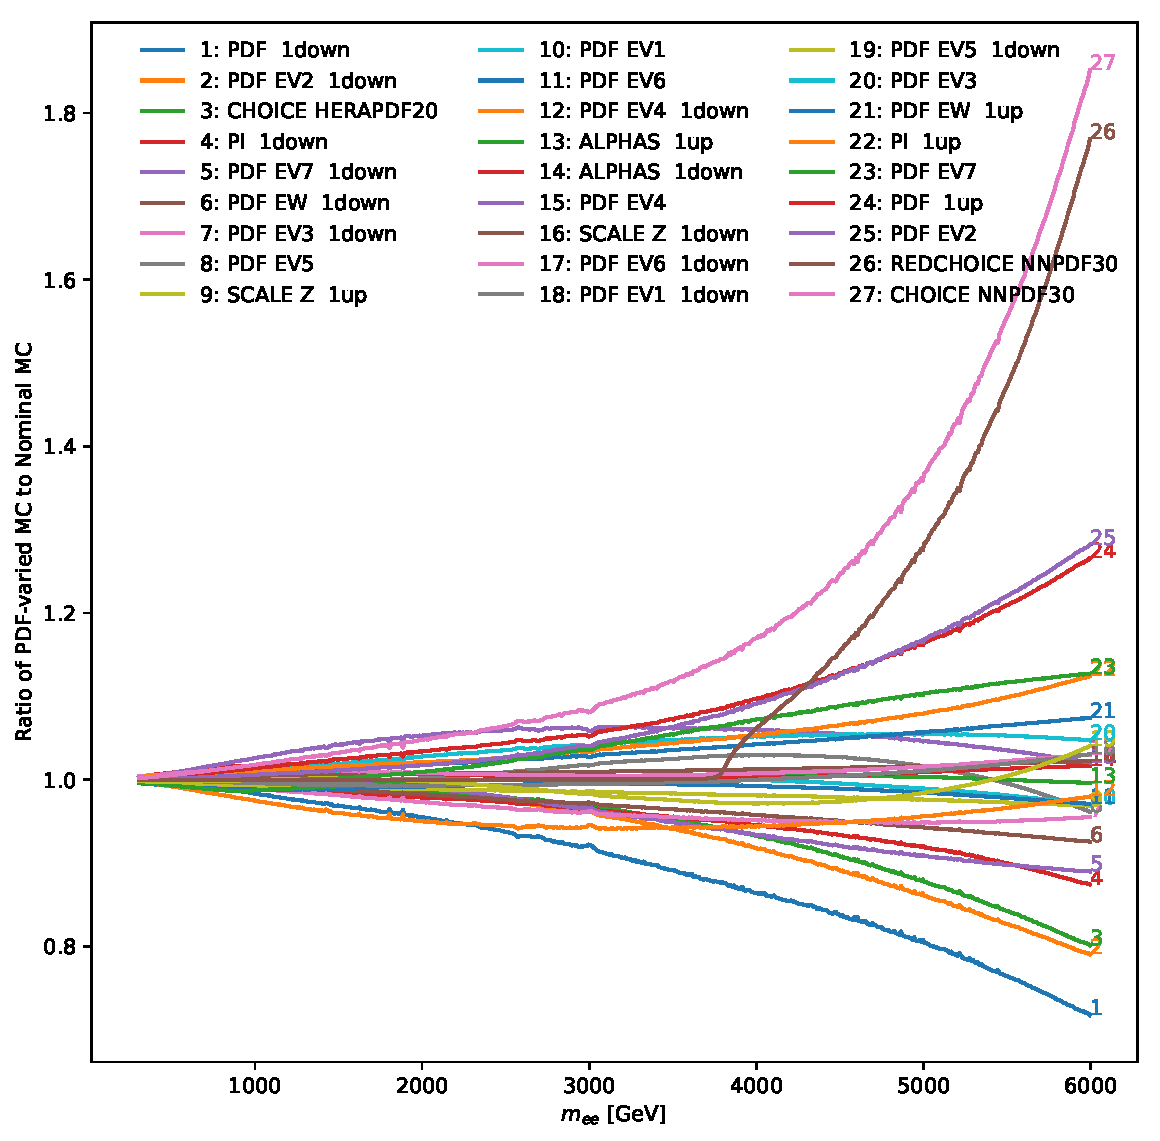
\includegraphics[width=0.45\textwidth]{figures/ci/bkgVarRatios/pdfComp-ee.pdf}}}
\subfloat[][]{{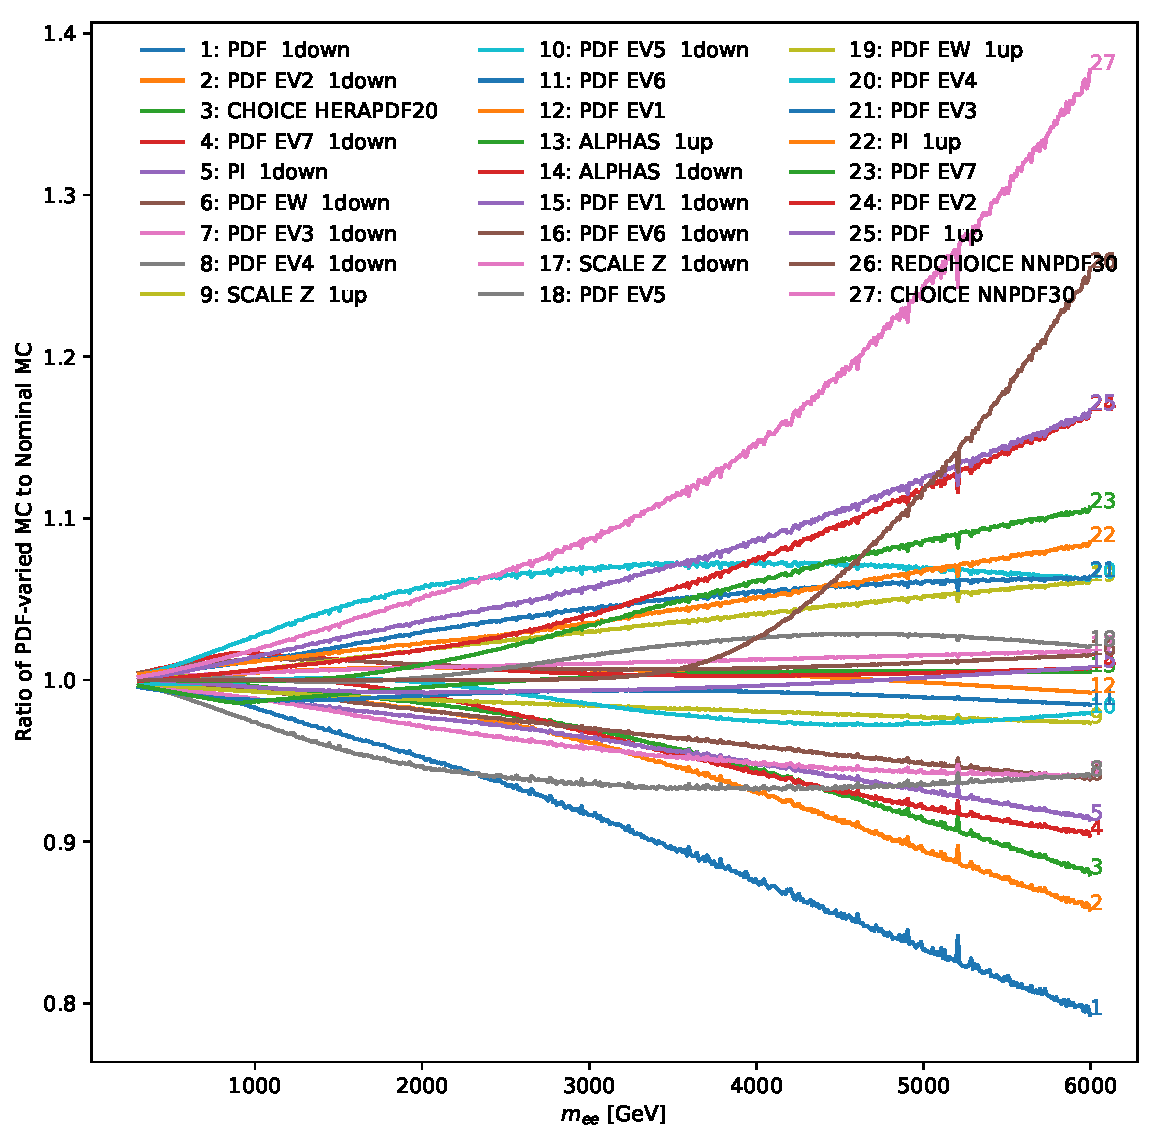
\includegraphics[width=0.45\textwidth]{figures/ci/bkgVarRatios/pdfComp-mm.pdf}}}
\caption{Illustration of theory variation shapes, shown as a ratio to the nominal MC, for $ee$ channel (a) and $\mu\mu$ channel (b). Two things are clear from these plots: the impact of the uncertainty in the PDF on $m_{ll}$, and that the impact grows with mass.}
\label{fig:ciThyVar}
\end{figure}

The following variations are considered for the theoretical uncertainties for the DY component only: the eigenvector variations of the nominal PDF set, variations of PDF scales, the strong coupling ($\alpha_{\textrm S}(M_Z)$), electroweak corrections, photon-induced corrections \cite{Martin:2005pi}, as well as the effect of choosing different PDF sets.
For all PDF variations, the modified DY component is used along with the other nominal background components.
These theoretical uncertainties are the same for both dilepton channels at generator level, but they result in different uncertainties at reconstruction level due to the different resolutions of the dielectron and dimuon channels.
% Further details of this procedure can be found in Ref.~\cite{EXOT-2016-05}.
The size of these uncertainties in the total simulated background is $\leq 19\%$ ($\leq 15\%$) below 4000~GeV for the dielectron (dimuon) channel.

The theoretical systematic uncertainties are used to produce variations on the invariant-mass spectra.
These are illustrated in Figure \ref{fig:ciThyVar}.


% \begin{table}[htp]
%     \centering
%     \begin{tabular}{c}
%     \toprule
%     PDF Variations \\
%     \midrule
%     ALPHAS \\
%     PDF EW \\
%     PI \\
%     PDF Eigenvector Variation 1 \\
%     PDF Eigenvector Variation 2 \\
%     PDF Eigenvector Variation 3 \\
%     PDF Eigenvector Variation 4 \\
%     PDF Eigenvector Variation 5 \\
%     PDF Eigenvector Variation 6 \\
%     PDF Eigenvector Variation 7 \\
%     SCALE Z \\
%     REDCHOICE NNPDF30 \\
%     CHOICE HERAPDF20  \\
%     CHOICE NNPDF30 \\
%     SCALE Z 1up \\
%     Without Run2 FakesTemplate \\
%     Run2 FakesTemplate x3 \\
%     Run2 FakesTemplate x2 \\
%     \bottomrule
%     \end{tabular}
%     \caption{Breakdown of variations of the nominal background included in the calculation of the ISS. These include the fake template variations, PDF choice, eigenvector and scale variations.}
%     \label{tab:ISSBreakdown}
% \end{table}

\subsubsection{Experimental Simulated Systematics}\ref{sec:ciExpSyst}

Uncertainty about the response and performance of the detector lead to systematic experimental uncertainties.
Among the experimental uncertainty sources in the dielectron channel, the dominant ones are the electron identification at low dielectron masses ($\leq 5\%$, below $\sim2000$~GeV) and the uncertainty in the electromagnetic energy scale at higher dielectron masses ($\leq 15\%$).
In the muon channel, the dominant experimental uncertainties arise from the muon reconstruction efficiency at low dimuon masses ($\leq 20\%$, below $\sim4000$~GeV) and from the identification of high-\pt muons at higher dimuon masses ($\leq 50\%$).
The full set of experimental uncertainties are illustrated for the electron channel in Figure \ref{fig:ciExpVarEe}, and for the muon channel in Figure \ref{fig:ciExpVarMm}.

\begin{figure}[htp]
\centering
\begin{overpic}[width=1\textwidth]{figures/ci/bkgVarRatios/pdfComp-ee-det.pdf}\put(85,0){}\end{overpic}
\caption{Ratio of the background variations to the nominal background estimate for the detector systematic variations in the electron channel. The prominent variations are numbered.}
\label{fig:ciExpVarEe}
\end{figure}

\begin{figure}[htp]
\centering
\begin{overpic}[width=1\textwidth]{figures/ci/bkgVarRatios/pdfComp-mm-det.pdf}\put(85,0){}\end{overpic}
\caption{Ratio of the background variations to the nominal background estimate for the detector systematic variations in the muon channel. The prominent variations are numbered.}
\label{fig:ciExpVarMm}
\end{figure}

\subsubsection{Multijet Electron Background}

The relative uncertainty of the simulated background due to the multi-jet and $W$+jets component rises from $\sim1\%$ at 1~TeV to $\sim10\%$ at 4~TeV.
For the multi-jet and $W$+jets component variations, the modified shape is used each time along with the other nominal background components from simulation.
This contribution is the smallest amongst all other variations in the CR.

\subsection{Background Estimate}\label{sec:ciSystBkg}
The background estimate describe in Section \ref{sec:ciBkg} predicts an event yield in the signal region, based on a functional form fit to the events observed in a control region.
Several assumptions are made in order to interpret this estimate as the prediction of the background hypothesis.
Each assumption is made with a degree of uncertainty.
This is quantified by the three systematic uncertainties described here: the extrapolation uncertainty, the induced spurious-signal (ISS) uncertainty, and the function bias uncertainty.

The extrapolation and ISS uncertainties are the dominant uncertainties on the background estimate.
These are both measured using statistical ensembles.

\subsubsection{Extrapolation Uncertainty}
\begin{figure}[h!]
\captionsetup[subfigure]{position=b}
\centering
\subfloat[][]{{\includegraphics[width=0.45\textwidth]{example-image-a}}}
\subfloat[][]{{\includegraphics[width=0.45\textwidth]{example-image-a}}} \\
\subfloat[][]{{\includegraphics[width=0.45\textwidth]{example-image-a}}}
\subfloat[][]{{\includegraphics[width=0.45\textwidth]{example-image-a}}}
\caption{Distributions of the differences between fits to the nominal dataset, and the toy datasets, for each SR.}
\label{fig:ciBkgEuSyst}
\end{figure}

The leading uncertainty on the estimated background is named the extrapolation uncertainty.
The functional form is fit in the CR to data collected in that region.
Since many events occupy each CR ($\approx$72k muons and $\approx$54k electrons), the shape of the \mll data distribution approximates the shape of the underlying truth-PDF that generated it.
However this approximation is not perfect due to statistical fluctuations in the CR.
The extrapolation uncertainty quantifies the degree to which statistical fluctuations in the CR may lead to varying background estimates in the SR.

This sort of uncertainty is present in other searches, and is sometimes called a ``function choice'' uncertainty.
Previously this has been estimated by comparing the result of choosing different functional forms to fit to the data.  {\color{red} [add citations, eg W']}
It is also possible to estimate this impact by looking at the constraints on and covariance of individual parameters of the functional form.
The procedure detailed here forgoes these estimates for a more direct measurement of the impact of statistical fluctuations on the estimated background.

To measure this impact, the background functional form is fit to the data in each CR.
This produces a smooth, \emph{nominal-PDF} that is the best available estimate of truth-PDF.
The background estimate from this fit in the SR defines $N_\text{bkg}^\text{Fit Nominal}$.
The nominal-PDF is used to generate an ensemble of \emph{pseudo-experiments}: toy datasets in the CR invariant-mass region with a multiplicity matching the dataset.
\footnote{There is no uncertainty as to the multiplicity of the actual dataset, and so this exactly determines the toy dataset multiplicity. An alternative option would be to allow $\sqrt{N}$ fluctuation of the multiplicity of each toys. In this case, the toy datasets correspond to the thought experiment: ``if Run 2 had been repeated, lasting for the same duration, what dataset may have been collected?'' This is not the precise thought experiment of interest. Instead, because a fixed number of events have already been sampled from the truth-PDF, it is asked: ``if an alternative sampling of the truth-PDF had taken place, what dataset may have been collected?''}
Each toy dataset is then fit using the background functional form and the resulting function is extrapolated to the SR to provide a toy background estimate $N_{\text{bkg},i}^\text{Fit Toy}$.
A comparison is made between the background estimate from the fit to the toy dataset and the nominal fit for each toy $i$:
\begin{equation*}
    \Delta_i^\text{stat}=N_{\text{bkg},i}^\text{Fit Toy}-N_\text{bkg}^\text{Fit Nominal}.
\end{equation*}
This defines the degree, $\Delta_i^\text{stat}$, to which statistical effects in the CR have altered the background estimate.


This procedure is repeated with an ensemble of 2000 toy datasets.
The distribution of $\Delta_i^\text{stat}$ values is built from each fit. These are shown in Figure \ref{eqn:ciBkgEuSyst} for each SR.
The standard deviation of these distributions is taken to define the systematic error on the background expectation due to the extrapolation uncertainty.

\subsubsection{Induced Spurious-Signal}
\begin{figure}[h!]
\captionsetup[subfigure]{position=b}
\centering
\subfloat[][]{{\includegraphics[width=0.45\textwidth]{example-image-a}}}
\subfloat[][]{{\includegraphics[width=0.45\textwidth]{example-image-a}}} \\
\subfloat[][]{{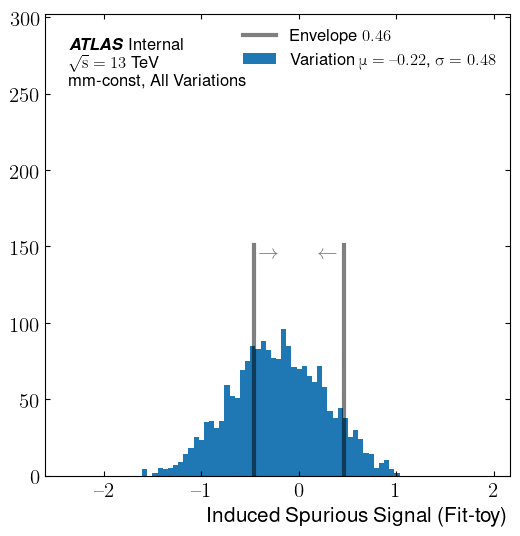
\includegraphics[width=0.45\textwidth]{figures/ci/iss/toyNSSDist-mm-const-all-noGaus.png}}}
\subfloat[][]{{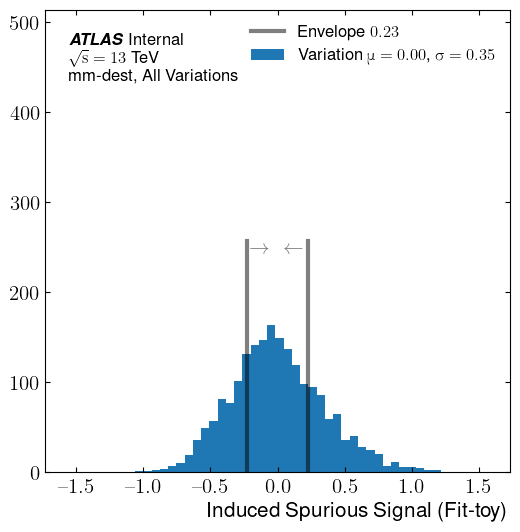
\includegraphics[width=0.45\textwidth]{figures/ci/iss/toyNSSDist-mm-dest-all-noGaus.png}}}
\caption{Distributions of the Induced Spurious-Signal.}
\label{fig:ciBkgIssSyst}
\end{figure}

% What needs to be measured
The sub-leading uncertainty on the background estimate is called the induced spurious-signal (ISS) uncertainty.
This quantifies the systematic difference between the background model and the true underlying background-only distribution in the SR.
The ISS how well the background model can be expected to model the underlying physical distribution from which the data has been sampled.
If the background functional form were to be fit to the true background-PDF, then the difference between the fitted function and normalized PDF in the CR is the ISS.
Since any missmodeling of the background, on average, leads to the identification of a signal even in the background-only scenario, this is missmodeling is called a \emph{spurious-signal}.

% Challenge with measuring it
The ISS can not be measured directly, since the background-PDF is unknown.
It is furthermore inaccurate to use the simulated background-only dataset to measure the ISS because this makes the improper assumption that the nominal simulation matches the shape of the true background-PDF.
Instead, a new methodology called the \emph{statistical background ensemble} was developed to measure the ISS.
The general theoretical motivation for the methodology is described in Appendix \ref{sec:backgroundEnsamble}.
The method seeks to measure the ISS from an ensemble of possible background shapes, each weighted by a prior likelihood.
The prior likelihoods are derived from the systematic variations discussed in Section \ref{sec:ciSystVars}.

The space of all plausible background shapes is described by linear combinations of the $n$ systematic variations.
Each of these is identified by a corresponding $n$-vector $\vec{\theta}$.
Each choice of $\vec{\theta}$ corresponds to a background shape $B'$:
\begin{equation}\begin{split}
    B'(\mll,\vec{\theta}) = B_\text{Nominal}(\mll) + \sum_{i=1}^n \omega_i(\mll)*\theta_i,
\end{split}\end{equation} 
where $\omega_i$ correspond to the shapes of the systematic variations.
The $\omega_i$ shapes can be normalized to correspond to $1\sigma$ deviations from the nominal shape.
In this case, $\theta_i=1$ corresponds to a $+1\sigma$ deviation, while $\theta_i=-1$ corresponds to a $-1\sigma$ deviation.
If the systematic variations are taken to define prior probabilities for nuisance parameters $\theta_i$, then the prior probability of $\vec{\theta}$ corresponding to the true background shape is:
\begin{equation}\begin{split}
    P(\vec{\theta})=\prod_{i=1}^n \text{G}(\theta_i),
\end{split}\end{equation} 
where $\text{G}(\theta_i)$ are standard normal functions.

In many cases, the systematic uncertainty shape is measured separately for upward and downward fluctuations.
For these systematics, the two shapes $\omega^+_i$ and $\omega^-_i$ are used as appropriate depending on whether $\theta_i$ is positive or negative.

Ideally, the ISS could be measured across the full space of $\vec{\theta}$.
This can be approximated numerically using an ensemble of backgrounds drawn from space of $\vec{\theta}$ randomly weighted by their prior likelihood.
For each of the $n$ systematic variations, a standard Gaussian PDF is sampled to determine the corresponding element of $\vec{\theta}$. \footnote{At the request of the ATLAS Publications Committee, the Gaussians are restricted to $[-1,1]$. This restriction is not impactful.}
The result is that each $\vec{\theta}$ of the ensemble is drawn with a probability proportional to the prior probability of the corresponding background shape.
Then, the background shapes $B'(\mll,\vec{\theta})$ and $B'(\mll,-\vec{\theta})$ are constructed.
The use of both $\vec{\theta}$ and $-\vec{\theta}$ forces a symmetric sampling of the space of $\vec{\theta}$. 
This reduces size of the ensemble required to sample the vector space.

This process is repeated to build an ensemble of background shapes, which are used to create 2000 Asimov toy datasets.
Each toy dataset is fit with the nominal background functional form.
A comparison is made between SR yields of the fitted function and the Asimov dataset for each toy $i$:
\begin{equation*}
    \Delta_i^\text{ISS}=N_{\text{bkg},i}^\text{Fit}-N_\text{bkg}^\text{Asimov}.
\end{equation*}
The distribution of $\Delta_i^\text{ISS}$ is built up through 2000 background shape toys for each SR, as shown in Figure \ref{fig:ciBkgIssSyst}.
The mean of these distributions defines the measurement of the ISS of the background model in each SR.
The width of these distributions is the uncertainty corresponding to that measurement.
The mean and standard deviation of the distribution are added in quadrature as the estimate of the ISS for the underlying background-PDF.

\subsubsection{Function Bias Uncertainty}

The final uncertainty on the background estimate is the function bias uncertainty.
This uncertainty constrains the degree to which a signal, if present in the CR, may bias the background expectation in the SR.
This is accomplished with the help of the S+B functional form of Equation \ref{eqn:ciSB}.
The results in Section \ref{sec:ciLinearity} establish that fits of the S+B functional form predict background yields in the SR that are not measurably distorted by the presence of a signal.
A comparison between the background expectations in the SR of the background-only and the S+B functional forms, when fitted to the data in the CR.
The difference between these two backgrounds expectations is taken to provide the function bias uncertainty.

The function bias uncertainty is small by construction.
If, when measured on data for a given control region, the value had been significant compared to extrapolation and ISS uncertainties, then this would have invalidated the choice of CR by indicating the presence of a signal-like feature.
In this case, a procedure was defined before unblinding the data in the SR.
The high-mass limit of the CR would be lowered until the bias vanished, with no adjustment to the SR. 
Because the non-resonant signals of interest vanish towards low-mass, reducing the upper limit of the CR would eventually remove the contribution from such a signal.

The results of the function bias measurement are shown in Figure \ref{fig:ciFuncBias}.
This measurement is repeated for each SR and for each chirality model.
A conservative choice of the largest bias for any given chirality is selected.
None of the function bias measurements are significant compared to the dominant uncertainties on the background model.
Indeed, the impact on the final results is under 2\%.

This uncertainty is only considered for the limits on the contact interaction energy scale \lam, since it depends on the shape of those signals.

\afterpage{
\begin{figure}[!htb]
\begin{center}
\subfloat[][]{{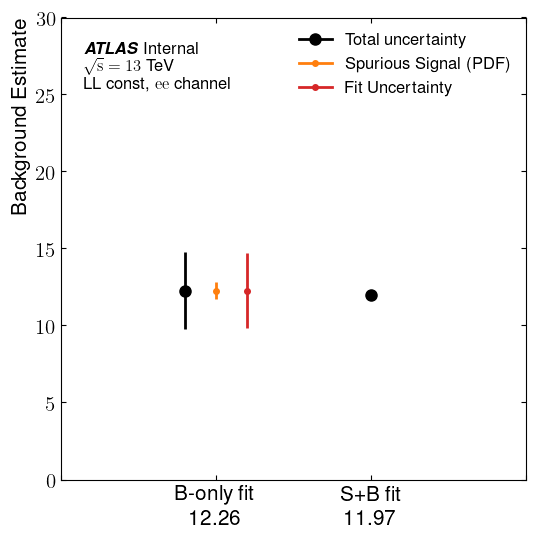
\includegraphics[width=0.24\textwidth]{figures/ci/bkgCompat-final/nbkg-LL-const-ee.png}}}
\subfloat[][]{{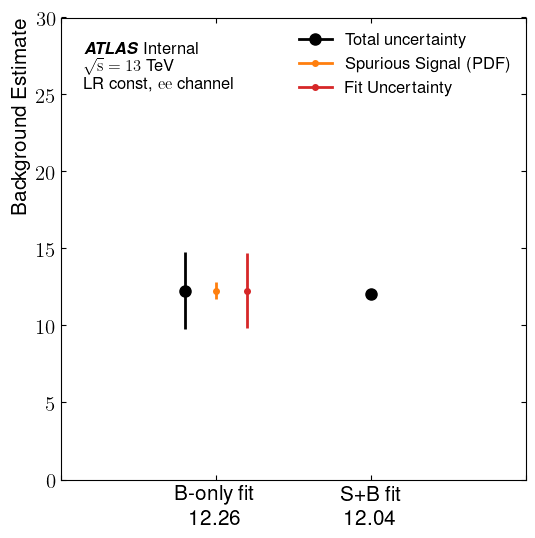
\includegraphics[width=0.24\textwidth]{figures/ci/bkgCompat-final/nbkg-LR-const-ee.png}}}
\subfloat[][]{{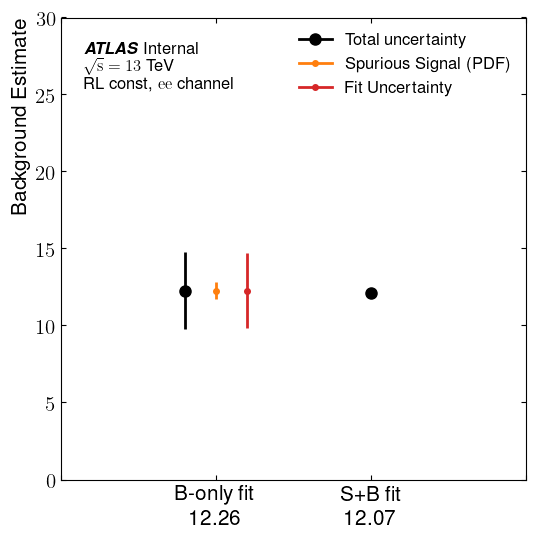
\includegraphics[width=0.24\textwidth]{figures/ci/bkgCompat-final/nbkg-RL-const-ee.png}}}
\subfloat[][]{{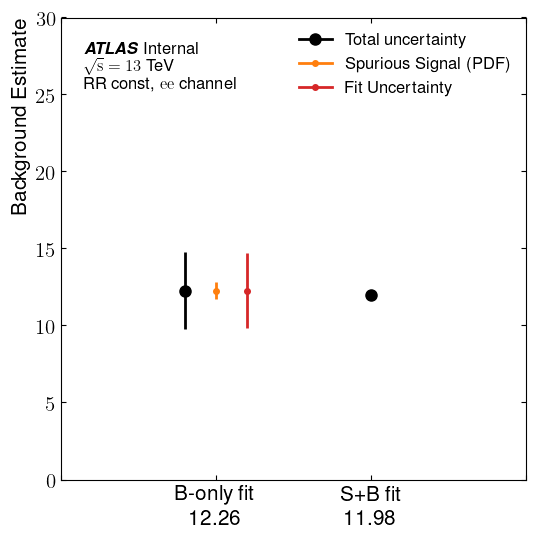
\includegraphics[width=0.24\textwidth]{figures/ci/bkgCompat-final/nbkg-RR-const-ee.png}}} \\
\subfloat[][]{{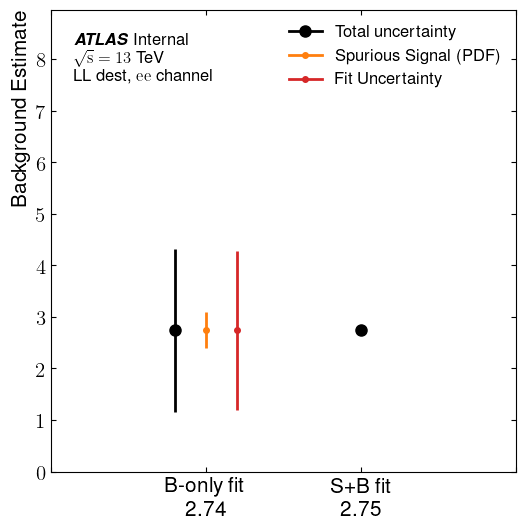
\includegraphics[width=0.24\textwidth]{figures/ci/bkgCompat-final/nbkg-LL-dest-ee.png}}}
\subfloat[][]{{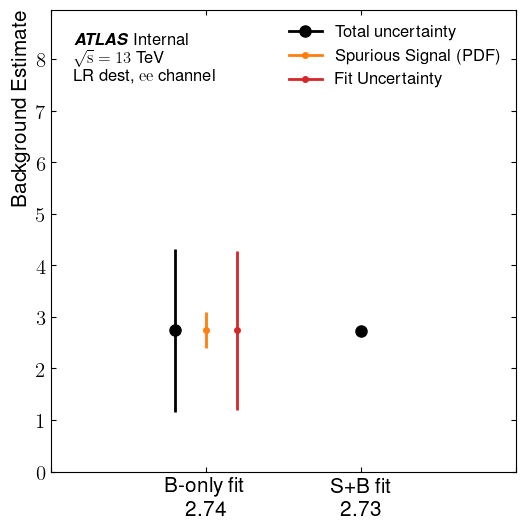
\includegraphics[width=0.24\textwidth]{figures/ci/bkgCompat-final/nbkg-LR-dest-ee.png}}}
\subfloat[][]{{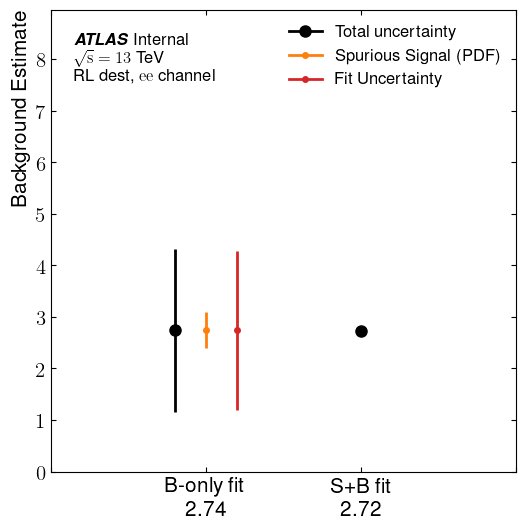
\includegraphics[width=0.24\textwidth]{figures/ci/bkgCompat-final/nbkg-RL-dest-ee.png}}}
\subfloat[][]{{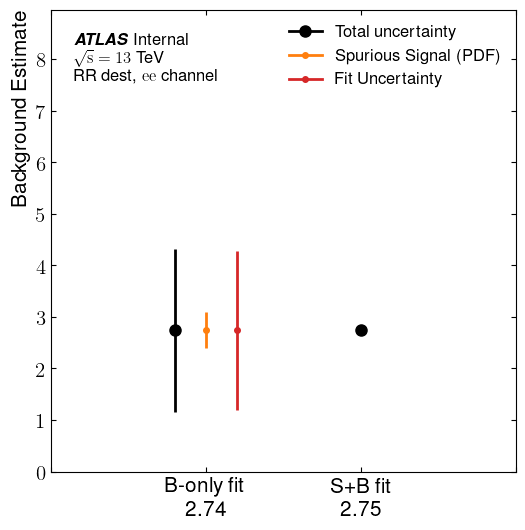
\includegraphics[width=0.24\textwidth]{figures/ci/bkgCompat-final/nbkg-RR-dest-ee.png}}} \\
\subfloat[][]{{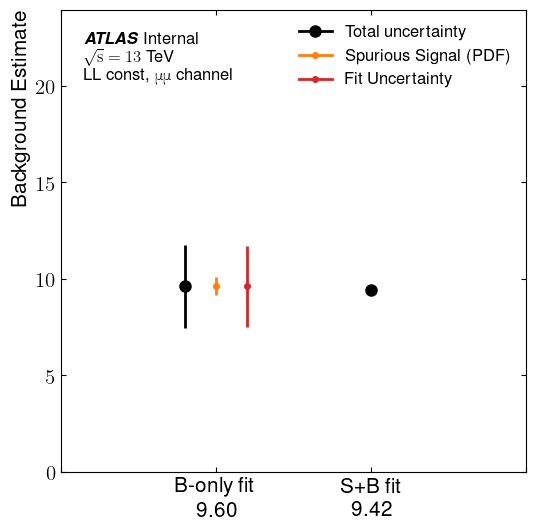
\includegraphics[width=0.24\textwidth]{figures/ci/bkgCompat-final/nbkg-LL-const-mm.png}}}
\subfloat[][]{{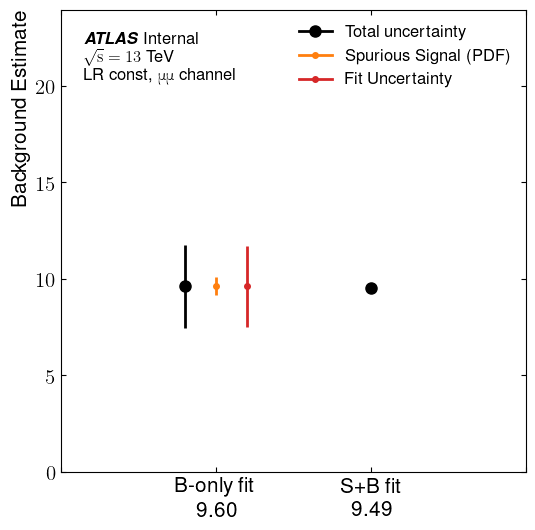
\includegraphics[width=0.24\textwidth]{figures/ci/bkgCompat-final/nbkg-LR-const-mm.png}}}
\subfloat[][]{{\includegraphics[width=0.24\textwidth]{figures/ci/bkgCompat-final/nbkg-RL-const-mm.png}}}
\subfloat[][]{{\includegraphics[width=0.24\textwidth]{figures/ci/bkgCompat-final/nbkg-RR-const-mm.png}}} \\
\subfloat[][]{{\includegraphics[width=0.24\textwidth]{figures/ci/bkgCompat-final/nbkg-LL-dest-mm.png}}}
\subfloat[][]{{\includegraphics[width=0.24\textwidth]{figures/ci/bkgCompat-final/nbkg-LR-dest-mm.png}}}
\subfloat[][]{{\includegraphics[width=0.24\textwidth]{figures/ci/bkgCompat-final/nbkg-RL-dest-mm.png}}}
\subfloat[][]{{\includegraphics[width=0.24\textwidth]{figures/ci/bkgCompat-final/nbkg-RR-dest-mm.png}}}
\caption{Background estimate compared in the SR, for B-only and S+B fits to data in each channel. (a-d) show constructive \ee fits for LL, LR, RL, and RR chiralities. (d-h) show the same for destructive \ee. (i-l) show the same for constructive \mm, and (m-p) show the same for destructive \mm.}
\label{fig:ciFuncBias}
\end{center}
\end{figure}
\clearpage
}


\subsection{Signal Model}\label{sec:ciSystSig}
The signal models used in this analysis are more traditional than the background model, and therefore the corresponding systematic uncertainties are fairly standard.
There are both experimental and theoretical uncertainties to consider.
The experimental uncertainties, described in Section \ref{sec:ciSigExpSyst}, are applied similarly to the CI signal model, and the model-independent signal production.
The theoretical uncertainties, described in Section \ref{sec:ciSigThySyst}, must be considered differently.
The hypothesis test performed by this analysis compares the background hypothesis to the signal+background hypothesis.
The choice of the signal model unambiguous: there is no uncertainty in what signal model is being tested.
Theoretical variations, like the PDF choice and $\alpha_s$ scale are part of this signal model choice.
Different theoretical choices describe different signal models.
Therefore, these different signal models are tested for in separate hypothesis tests.

\subsubsection{Experimental}\label{sec:ciSigExpSyst}

The experimental uncertainties under consideration are described in Section \ref{sec:ciExpSyst}.
These are produced as functions of invariant-mass \mll.
The impact of each systematic on the CI signal model is the convolution of the CI shape in \mll and the systematic shape in \mll, but this is relatively independent of the signal shape.
For different contact interactions, the impact of experimental systematics generally varies by less than 1\%.
Thus for simplicity these are calculated for the LO DY shape in the CR and applied equally for each CI model.
The experimental uncertainties are given in Table \ref{tab:ciExpVariationBonanza}.
The sum in quadrature of the experimental uncertainties is used to constrain the signal prediction.
The experimental uncertainties of the signal are $\leq 9\%$ for the electron channel and $\leq 22\%$ for the muon channel.

\afterpage{
\begin{table}[]
\begin{center}
\caption{Impact of experimental uncertainties on NLO DY yield in CI signal regions. The sum in quadruature row includes only contributions from sources of impact $\geq 1\%$.}
\tiny
\begin{tabular}{|c|c|c|c|}
\hline
\hline
Process & Signal region & Uncertainty & \# events in SR \\
\hline
DY$\rightarrow ee$ & const. ($m_{ee} \geq 2200$ GeV) & nominal & $0.9824$ \\
DY$\rightarrow ee$ & const. ($m_{ee} \geq 2200$ GeV) & EG\_RES & $\sim 0.0\% \ \sim 0.0\%$ \\
DY$\rightarrow ee$ & const. ($m_{ee} \geq 2200$ GeV) & EG\_SCALE & $+ 5.9\% \   -5.8\%$ \\
DY$\rightarrow ee$ & const. ($m_{ee} \geq 2200$ GeV) & EL\_ChargeID & $\sim 0.0\% \ \sim 0.0\%$ \\
DY$\rightarrow ee$ & const. ($m_{ee} \geq 2200$ GeV) & EL\_ID & $+ 5.9\% \   -5.8\%$ \\
DY$\rightarrow ee$ & const. ($m_{ee} \geq 2200$ GeV) & EL\_Iso & $+ 0.8\% \   -0.8\%$ \\
DY$\rightarrow ee$ & const. ($m_{ee} \geq 2200$ GeV) & EL\_Reco & $+ 0.4\% \   -0.4\%$ \\
DY$\rightarrow ee$ & const. ($m_{ee} \geq 2200$ GeV) & EL\_TRIG\_EFF & $\sim 0.0\% \ \sim 0.0\%$ \\
DY$\rightarrow ee$ & const. ($m_{ee} \geq 2200$ GeV) & EL\_TRIG\_TOTAL & $\sim 0.0\% \ \sim 0.0\%$ \\
DY$\rightarrow ee$ & const. ($m_{ee} \geq 2200$ GeV) & PRW & $\sim 0.0\% \   -0.1\%$ \\
\hline
 & & Quad. sum (impact $\geq 1\%$) & $+ 8.4\% \   -8.2\%$ \\
\hline
DY$\rightarrow ee$ & dest. ($m_{ee} \geq 2770$ GeV) & nominal & $4.4867$ \\
DY$\rightarrow ee$ & dest. ($m_{ee} \geq 2770$ GeV) & EG\_RES & $\sim 0.0\% \ \sim 0.0\%$ \\
DY$\rightarrow ee$ & dest. ($m_{ee} \geq 2770$ GeV) & EG\_SCALE & $+ 5.2\% \   -4.9\%$ \\
DY$\rightarrow ee$ & dest. ($m_{ee} \geq 2770$ GeV) & EL\_ChargeID & $\sim 0.0\% \ \sim 0.0\%$ \\
DY$\rightarrow ee$ & dest. ($m_{ee} \geq 2770$ GeV) & EL\_ID & $+ 5.9\% \   -5.8\%$ \\
DY$\rightarrow ee$ & dest. ($m_{ee} \geq 2770$ GeV) & EL\_Iso & $+ 0.8\% \   -0.8\%$ \\
DY$\rightarrow ee$ & dest. ($m_{ee} \geq 2770$ GeV) & EL\_Reco & $+ 0.4\% \   -0.4\%$ \\
DY$\rightarrow ee$ & dest. ($m_{ee} \geq 2770$ GeV) & EL\_TRIG\_EFF & $\sim 0.0\% \ \sim 0.0\%$ \\
DY$\rightarrow ee$ & dest. ($m_{ee} \geq 2770$ GeV) & EL\_TRIG\_TOTAL & $\sim 0.0\% \ \sim 0.0\%$ \\
DY$\rightarrow ee$ & dest. ($m_{ee} \geq 2770$ GeV) & PRW & $\sim 0.0\% \ \sim 0.0\%$ \\
\hline
 & & Quad. sum (impact $\geq 1\%$) & $+ 7.9\% \   -7.6\%$ \\
\hline
\hline
DY$\rightarrow \mu\mu$ & const. ($m_{\mu\mu} \geq 2070$ GeV) & nominal & $1.3524$ \\
DY$\rightarrow \mu\mu$ & const. ($m_{\mu\mu} \geq 2070$ GeV) & MUON\_BADMUON\_STAT & $\sim 0.0\% \ \sim 0.0\%$ \\
DY$\rightarrow \mu\mu$ & const. ($m_{\mu\mu} \geq 2070$ GeV) & MUON\_BADMUON\_SYS & $+ 7.8\% \   -7.6\%$ \\
DY$\rightarrow \mu\mu$ & const. ($m_{\mu\mu} \geq 2070$ GeV) & MUON\_ISO\_STAT & $+ 0.3\% \   -0.3\%$ \\
DY$\rightarrow \mu\mu$ & const. ($m_{\mu\mu} \geq 2070$ GeV) & MUON\_ISO\_SYS & $+ 0.4\% \   -0.4\%$ \\
DY$\rightarrow \mu\mu$ & const. ($m_{\mu\mu} \geq 2070$ GeV) & MUON\_RECO\_STAT & $+ 0.6\% \   -0.6\%$ \\
DY$\rightarrow \mu\mu$ & const. ($m_{\mu\mu} \geq 2070$ GeV) & MUON\_RECO\_SYS & $+ 21.7\% \   -19.4\%$ \\
DY$\rightarrow \mu\mu$ & const. ($m_{\mu\mu} \geq 2070$ GeV) & MUON\_TTVA\_STAT & $\sim 0.0\% \ \sim 0.0\%$ \\
DY$\rightarrow \mu\mu$ & const. ($m_{\mu\mu} \geq 2070$ GeV) & MUON\_TTVA\_SYS & $\sim 0.0\% \ \sim 0.0\%$ \\
DY$\rightarrow \mu\mu$ & const. ($m_{\mu\mu} \geq 2070$ GeV) & MUON\_TRIG\_STAT & $\sim 0.0\% \ \sim 0.0\%$ \\
DY$\rightarrow \mu\mu$ & const. ($m_{\mu\mu} \geq 2070$ GeV) & MUON\_TRIG\_SYS & $+ 0.1\% \   -0.1\%$ \\
DY$\rightarrow \mu\mu$ & const. ($m_{\mu\mu} \geq 2070$ GeV) & MUON\_ID & $+ 1.0\% \   -1.1\%$ \\
DY$\rightarrow \mu\mu$ & const. ($m_{\mu\mu} \geq 2070$ GeV) & MUON\_MS & $+ 4.6\% \   -3.7\%$ \\
DY$\rightarrow \mu\mu$ & const. ($m_{\mu\mu} \geq 2070$ GeV) & MUON\_SAGITTA\_RESBIAS & $+ 12.8\% \ + 5.5\%$ \\
DY$\rightarrow \mu\mu$ & const. ($m_{\mu\mu} \geq 2070$ GeV) & MUON\_SAGITTA\_RHO & $\sim 0.0\% \ \sim 0.0\%$ \\
DY$\rightarrow \mu\mu$ & const. ($m_{\mu\mu} \geq 2070$ GeV) & MUON\_SCALE & $  -0.4\% \ + 0.3\%$ \\
DY$\rightarrow \mu\mu$ & const. ($m_{\mu\mu} \geq 2070$ GeV) & PRW & $\sim 0.0\% \ \sim 0.0\%$ \\
\hline
 & & Quad. sum (impact $\geq 1\%$) & $+ 26.7\% \   -21.9\%$ \\
\hline
DY$\rightarrow \mu\mu$ & dest. ($m_{\mu\mu} \geq 2570$ GeV) & nominal & $4.7216$ \\
DY$\rightarrow \mu\mu$ & dest. ($m_{\mu\mu} \geq 2570$ GeV) & MUON\_BADMUON\_STAT & $\sim 0.0\% \ \sim 0.0\%$ \\
DY$\rightarrow \mu\mu$ & dest. ($m_{\mu\mu} \geq 2570$ GeV) & MUON\_BADMUON\_SYS & $+ 4.0\% \   -3.8\%$ \\
DY$\rightarrow \mu\mu$ & dest. ($m_{\mu\mu} \geq 2570$ GeV) & MUON\_ISO\_STAT & $+ 0.3\% \   -0.2\%$ \\
DY$\rightarrow \mu\mu$ & dest. ($m_{\mu\mu} \geq 2570$ GeV) & MUON\_ISO\_SYS & $+ 0.5\% \   -0.3\%$ \\
DY$\rightarrow \mu\mu$ & dest. ($m_{\mu\mu} \geq 2570$ GeV) & MUON\_RECO\_STAT & $+ 0.6\% \   -0.5\%$ \\
DY$\rightarrow \mu\mu$ & dest. ($m_{\mu\mu} \geq 2570$ GeV) & MUON\_RECO\_SYS & $+ 17.9\% \   -16.1\%$ \\
DY$\rightarrow \mu\mu$ & dest. ($m_{\mu\mu} \geq 2570$ GeV) & MUON\_TTVA\_STAT & $+ 0.1\% \ \sim 0.0\%$ \\
DY$\rightarrow \mu\mu$ & dest. ($m_{\mu\mu} \geq 2570$ GeV) & MUON\_TTVA\_SYS & $\sim 0.0\% \ \sim 0.0\%$ \\
DY$\rightarrow \mu\mu$ & dest. ($m_{\mu\mu} \geq 2570$ GeV) & MUON\_TRIG\_STAT & $+ 0.2\% \ \sim 0.0\%$ \\
DY$\rightarrow \mu\mu$ & dest. ($m_{\mu\mu} \geq 2570$ GeV) & MUON\_TRIG\_SYS & $+ 0.2\% \ \sim 0.0\%$ \\
DY$\rightarrow \mu\mu$ & dest. ($m_{\mu\mu} \geq 2570$ GeV) & MUON\_ID & $+ 0.7\% \   -0.7\%$ \\
DY$\rightarrow \mu\mu$ & dest. ($m_{\mu\mu} \geq 2570$ GeV) & MUON\_MS & $+ 2.7\% \   -2.2\%$ \\
DY$\rightarrow \mu\mu$ & dest. ($m_{\mu\mu} \geq 2570$ GeV) & MUON\_SAGITTA\_RESBIAS & $+ 8.0\% \ + 1.8\%$ \\
DY$\rightarrow \mu\mu$ & dest. ($m_{\mu\mu} \geq 2570$ GeV) & MUON\_SAGITTA\_RHO & $\sim 0.0\% \ \sim 0.0\%$ \\
DY$\rightarrow \mu\mu$ & dest. ($m_{\mu\mu} \geq 2570$ GeV) & MUON\_SCALE & $  -0.4\% \ + 0.4\%$ \\
DY$\rightarrow \mu\mu$ & dest. ($m_{\mu\mu} \geq 2570$ GeV) & PRW & $\sim 0.0\% \ + 0.2\%$ \\
\hline
\hline
\end{tabular}
\label{tab:ciExpVariationBonanza}
\end{center}
\end{table}
\clearpage
}

\subsubsection{Theoretical}\label{sec:ciSigThySyst}
The theoretical uncertainties under consideration are described in Section \ref{sec:ciThySyst}.
These are useful in order to provide alternative signal models that correspond to the $1\sigma$ limits on theoretical parameters.
The impact of the theoretical uncertainties on the signal yield is calculated in each SR.
It is equal to the sum in quadrature of the convolution of the theory systematic shapes with the LO DY shape.


\subsection{Summary}

The numerical values of the uncertainties are given in Table \ref{tab:ciUncerts}.
For all cases, the relative uncertainties in the destructive SRs are larger than those in the constructive SRs.
This is due to both the smaller size of the SR leading to less background and hence larger relative uncertainty, and the smaller size of the CR leading to a weaker constraint on the background model.
For the background estimates, the leading uncertainty in each SR is the extrapolation uncertainty, followed by the ISS uncertainty.
Many of the experimental and theoretical systematics are measured separately for upward and downward fluctuations.


\begin{table}[!h]
\begin{center}
\caption{Summary of the relative uncertainties in the background estimate and signal in each SR, where EU is the `extrapolation uncertainty', ISS is the `induced spurious-signal uncertainty' and FB is the `function bias uncertainty'. Experimental and theoretical uncertainties are shown as well, with the latter averaged across CI chirality scenarios and quoted for $\Lambda=30$~TeV only.}
\begingroup
\setlength{\tabcolsep}{10pt} % Default value: 6pt
\renewcommand{\arraystretch}{1.5} % Default value: 1
{\small
% \begin{tabular}{l l | r r r | r r r r}
\begin{tabular}{l l | r r r | r@{}l r@{}l}
% \Xhline{2\arrayrulewidth}
\toprule
\multirow{2}{*}{Channel} & \multirow{2}{*}{Interference} & \multicolumn{3}{c|}{Background uncertainties} & \multicolumn{4}{c}{Signal uncertainties}\\
        &              & $\sigma_b^\text{EU}$ & $\sigma_b^\text{ISS}$ & $\sigma_b^\text{FB}$ & \multicolumn{2}{c}{$\sigma_s^\text{Experiment}$} & \multicolumn{2}{c}{$\sigma_s^\text{Theory}$} \\
\midrule
\ee     & Constructive & 14\% & 4\%  & 2\% & 8&\%                               & \makecell[r]{+11 \\ --10}&\makecell[l]{\% \\ \%} \\
\ee     & Destructive  & 34\% & 7\% & 1\%  & 8&\%                               & \makecell[r]{+14 \\ --13}&\makecell[l]{\% \\ \%} \\
$\mm$ & Constructive & 21\% & 6\%  & 2\% & \makecell[r]{+20 \\ --17}&\makecell[l]{\% \\ \%} & \makecell[r]{+10 \\ --9}&\makecell[l]{\% \\ \%} \\
$\mm$ & Destructive  & 58\% & 24\% & 4\% & \makecell[r]{+27 \\ --22}&\makecell[l]{\% \\ \%} & \makecell[r]{+13 \\ --12}&\makecell[l]{\% \\ \%} \\
% \Xhline{2\arrayrulewidth}
\bottomrule
\end{tabular}
}
\endgroup
\label{tab:ciUncerts}
\end{center}
\end{table}

\section{Statistical Analysis}\label{sec:ciStat}

Statistical methods are used to distill two types of information from the collected dataset.
First, what is the probability that the observed data is incompatible with the background-only hypothesis.
Second, what is smallest putative signal such that, if extant, would produce a signal+background hypothesis that is incompatible with the observed data.
The former is answered by a significance test, described in Section \ref{sec:ciSigTest}, while the latter is answered by setting a limit, described in Section \ref{sec:ciLimitSetting}.

\subsection{CLs}

The fundamental tool used to compare two hypotheses is the \emph{test statistic}.
While this can be any quantity calculated from data, an optimal choice for the test statistic may be made to best resolve the difference between the two hypotheses.
The Neyman-Person lemma states that the likelihood ratio test is the most likely to reject the null hypotheses given the alternate hypotheses is true.
The likelihood ratio is defined:
\begin{equation}\begin{split}
\Lambda(x)=\frac{\mathcal{L}(\theta_1|x)}{\mathcal{L}(\theta_0|x)},
\end{split}\end{equation} 
where $\mathcal{L}(\theta_0|x)$ and $\mathcal{L}(\theta_1|x)$ are the likelihoods to observe data $x$ under the null and alternate hypotheses, respectively.
Data measured at larger values of $\Lambda(x)$ are \emph{less compatible} with the background hypothesis.

The PDF of $\Lambda(x)$ is defined under both the null and alternate hypotheses.
Taking first the PDF under the null hypothesis, $\Lambda_0(x)$.
The integral of the test statistic $\Lambda_0(x)$ above a given observed value of $x$, $x_\text{obs}$, defines the \emph{p-value} $p_0$ of the observation.
This is the probability to observe a value of $x$ that is \emph{less} compatible with the null hypothesis than the observed value.
The complement of the p-value, calculated under the null hypothesis, defines the value $\clb\equiv1-p_0$.
An analogous value, $\clsb$, is defined for the likelihood ratio under the alternative hypothesis, $\Lambda_1(x)$.
For a measured $x_\text{obs}$, $p_1$ is the integral of $\Lambda_1(x)$ above that point, and $\clsb\equiv1-p_1$
Finally the ratio of these two values defines $\cls\equiv \clsb/\clb$.
The motivation 

\subsection{Statistical Model}

Each statistical question is answered through the comparison of null and alternate hypotheses.
% The 


\subsection{Significance test}\label{sec:ciSigTest}

A hypothesis test is performed in each of the four signal regions of the analysis.
The null hypothesis predicts the number of background events in the signal region, using the integral of the extrapolated fitted background-only functional form (Equations \ref{eqn:ciBkgEe} and \ref{eqn:ciBkgMm}).
The alternative hypothesis predicts the same number of background events as the null hypothesis, with the addition of a number of signal events.
The alternative hypothesis is fit to the observed data.


\subsection{Limit test}\label{sec:ciLimitSetting}

\section{Results}\label{sec:ciResults}

This analysis inspects the high-mass tails of the \ee and \mm invariant mass spectra.
Four signal regions are considered, two each for \ee and \mm selections.
For each signal region, the differential mass distribution in a lower mass control region is fit to produce a background estimate in the signal region.
This section presents the statistical investigation performed on the observation in each signal region and their physical interpretation.

\subsection{Data}

The data collected and analyzed is presented here for each signal region. 
First Table \ref{tab:ciData} presents the data and background expectations, along with the significance of the background-only hypothesis in each SR.

\begin{table}[H]
    \centering
    \begin{tabular}{l   r r@{}l c }
    \toprule
    \multicolumn{1}{c}{SR} & Data & \multicolumn{2}{c}{Background} & Significance \\
    \midrule
    \ee   Constructive & 19 & 12.4 & $\pm1.9$ & ~~~1.28 \\
    \ee   Destructive  & 2  & 3.1  & $\pm1.1$  & --~0.72 \\
    \midrule
    \mm Constructive & 6  & 9.6  & $\pm2.1$  & --~0.99 \\
    \mm Destructive  & 1  & 1.4  & $\pm0.9$  & --~0.58 \\
    \bottomrule
    \end{tabular}
    \caption{The dielectron and dimuon event yields for the data, the expected background and the respective significance in the different SRs used in the analysis.  The p-value of each observation is defined as the probability, given the background-only hypothesis, of an observation at least as large as that seen in the data.  The significance is the Gaussian cumulative density function of the p-value, and negative significances correspond to deficits. }
    \label{tab:ciData}
\end{table}

Small deficits compared to the expected background, are seen in the \mm SRs and the \ee destructive SR.
A moderate excess is observed in the \ee constructive SR.
None of these significances are judged to be significant enough to reject the background-only hypothesis.

\afterpage{
\begin{figure}[h!]
\centering
\subfloat[][]{{\includegraphics[width=0.5\textwidth]{figures/ci/results/fig_02a.pdf}}} % will be fig_02a.pdf
\subfloat[][]{{\includegraphics[width=0.5\textwidth]{figures/ci/results/fig_02b.pdf}}}\\ % will be fig_02b.pdf
\subfloat[][]{{\includegraphics[width=0.5\textwidth]{figures/ci/results/fig_02c.pdf}}} % will be fig_02c.pdf
\subfloat[][]{{\includegraphics[width=0.5\textwidth]{figures/ci/results/fig_02d.pdf}}} % will be fig_02d.pdf
\caption{
Distributions of the invariant mass of dilepton pairs passing the full selection for dielectrons (left) and dimuons (right), and showing CR and SR for constructive interference (top) and destructive interference (bottom).
Figures (c) and (d) show the region between the SR and CR, but the fit does not use this.
The data points are plotted at the center of each bin as the number of events divided by the bin width, which is constant in $\log{(m_{\ell\ell})}$.
The error bars indicate statistical uncertainties only.
A few CI benchmark signal shapes are shown, scaled to the data luminosity, and superimposed by subtracting the LO DY component and adding the resulting shape to the background shape obtained from the fit.
These signals have LL chirality with $\Lambda=$ 18, 22, and 26~TeV for the constructive case and $\Lambda=$16, 20, and $26$~TeV for the destructive case.
The background-only fit is shown in solid red, with the light red area being its uncertainty.
The boundaries of the CR and SR corresponding to the signals used are shown in dotted vertical lines for reference and marked by arrows.
%In the destructive interference case, the signal shapes do not differ much on the scale used for these plots.
The differences between the data and the fit results in units of standard deviations of the statistical uncertainty are shown in the bottom panels.
}
\label{fig:ciDist}
\end{figure}
\clearpage
}

The signal regions and control regions are illustrated in the plots of Figure \ref{fig:ciDist}.
Several observations follow.
First, the agreement between the fitted background function and the data is consistent in each CR.
The agreement is also reasonable in the gap between the CR and destructive SRs.
Next, the excesses and deficits listed in Table \ref{tab:ciData} appear in the signal regions of the plots.
For comparison, the predictions of several CI signal models are imposed on top of the background estimate.

The parameters of the fitted background shape are given in Table \ref{tab:fitpars}.
\begin{table}[htp]
\centering
\caption{Parameters for the functional form given in Equations \ref{eqn:ciBkgEe} and \ref{eqn:ciBkgMm}. The uncertainties are statistical only.}
{\footnotesize
 \begin{tabular}{l  r@{}c@{}l r@{}c@{}l  r@{}c@{}l r@{}c@{}l }
\toprule
Parameter  &  \multicolumn{3}{c}{\ee Constructive} &  \multicolumn{3}{c}{\ee Destructive} &  \multicolumn{3}{c}{\mm Constructive} &  \multicolumn{3}{c}{\mm Destructive} \\
\midrule
 Normalization & \multicolumn{3}{c}{$(6.17 \pm 0.02)\times 10^\text{-3}$} & \multicolumn{3}{c}{$(7.87\pm 0.03)\times 10^\text{-3}$} & \multicolumn{3}{c}{$(6.90\pm 0.03)\times 10^\text{-6}$} & \multicolumn{3}{c}{$(4.39\pm 0.02)\times 10^\text{-7}$} \\
 b (fixed) & \multicolumn{3}{c}{6.1} & \multicolumn{3}{c}{6.1} & \multicolumn{3}{c}{1.3} & \multicolumn{3}{c}{1.3} \\
 % c (fixed) & \multicolumn{3}{c}{1/2} & \multicolumn{3}{c}{1/2} & \multicolumn{3}{c}{1/3} & \multicolumn{3}{c}{1/3} \\
 $p_0$ &  ~~~~-12.2   & $\pm$ & 0.1       & ~~~~~-12.1  &$\pm$& 0.1   & ~~~~~-14.9  &$\pm$& 0.2   & ~~~~~-17.0 &$\pm$& 0.2 \\
 $p_1$ &  ~~~~-4.14   & $\pm$ & 0.02      & ~~~~~-4.16  &$\pm$& 0.03  & ~~~~~-4.42 &$\pm$& 0.04  &  ~~~~~-4.70 &$\pm$& 0.04 \\
 $p_2$ &  ~~~~-0.948  & $\pm$ & 0.005     & ~~~~~-0.945 &$\pm$& 0.006 & ~~~~~-0.927 &$\pm$& 0.008 & ~~~~~-0.846 &$\pm$& 0.008 \\
 $p_3$ &  ~~~~-0.0840 & $\pm$ & 0.0008    & ~~~~~-0.082 &$\pm$& 0.001 & ~~~~~-0.081 &$\pm$& 0.001 & ~~~~~-0.064 &$\pm$& 0.001 \\
\bottomrule\end{tabular}}
\label{tab:fitpars}
\end{table}

Although the background expectations from the simulation are not used explicitly for hypothesis tests, they are provided in Table \ref{tab:ciMcVsFit} along with the nominal background expectations.
The systematic uncertainty on the simulated \nbkg takes into account experimental and theoretical uncertainties, however, and these are not well known in the SR.
No significant difference is observed between the nominal background estimate and the simulated background estimate.

\begin{table}[H]
\centering
\caption{Comparison between the background estimate in the SR, as derived from fitting the data ($N_\text{fit}$), and the estimation from simulated background ($N_\text{sim}$). The yields observed in data ($N_\text{obs}$) are also given. All systematic uncertainties are included.}
\begin{tabular}{l | r r r }\toprule
SR & $N_\text{sim}\pm\sigma_\text{sim}$ & $N_\text{fit}\pm\sigma_\text{fit}$ & $N_\text{obs}$ \\
\hline
\ee Constructive   & $13.3  \pm 1.9$  & $12.4 \pm 1.9$ & 19 \\
\ee Destructive    & $2.9   \pm 0.6$  & $3.1  \pm 1.1$ & 2  \\ % fixed ee
\mm Constructive & $11.9  \pm 2.8$  & $9.6  \pm 2.1$ & 6  \\
\mm Destructive  & $3.3   \pm 1.0$  & $1.4  \pm 0.9$ & 1  \\
\bottomrule\end{tabular}\\ %remember cline{1-2}
\label{tab:ciMcVsFit}
\end{table}


A further comparison of the background differential shapes made in Figure \ref{fig:ciCiFitVsMc}.
These plots show a comparison between the fitted background function and the simulated background distribution in both the CR and SR.
The fitted background function is produced using the fit to data, not the simulation.

\begin{figure}[!htpb]
\centering
\subfloat[][]{{\includegraphics[width=0.45\textwidth]{figures/ci/results/figaux_08a.pdf}}}
\subfloat[][]{{\includegraphics[width=0.45\textwidth]{figures/ci/results/figaux_08b.pdf}}} \\
\subfloat[][]{{\includegraphics[width=0.45\textwidth]{figures/ci/results/figaux_08c.pdf}}}
\subfloat[][]{{\includegraphics[width=0.45\textwidth]{figures/ci/results/figaux_08d.pdf}}}
\caption{Fits performed on data (red) are compared to the background simulation. The background simulation is used only to study performance and systematics. The uncertainties on the background simulation are theory only, and are provided as a rough estimate.
Shown for \ee constructive (a), \ee destructive (b), \mm constructive (c), and \mm destructive (d).}
\label{fig:ciCiFitVsMc}
\end{figure}




\subsection{Limits on signal events}\label{sec:limNSig}

\begin{figure}[h!]
\begin{center}
\includegraphics[width=0.5\linewidth]{figures/ci/results/fig_03a.pdf}
\end{center}
\vspace{-.4cm}
\caption{Limits on the number of signal events in the respective signal region for each model. }
\label{fig:ciCiLimNSig}
\end{figure}

In the absence of significant deviations of the data from the background expectation, the observations are used to set limits on signal production in each SR.
The limits in this section use the hypotheses defined in Equations \ref{eqn:ciNullLikelihoodNSig} and \ref{eqn:ciAltLikelihoodNSig}.
The parameter of interest is the number of signal events to pass the event selection, \nsig.
This is trivially converted to limits on the visible component of a signal production mechanism, \xsbr, with the division by the integrated luminosity.
The expected and observed upper limits on both \nsig and \xsbr at 95\% confidence level are given in Table \ref{tab:ciNsigLimits}.
Because these limits do not make strict assumptions about the signal production mechanism, they can be directly reinterpreted for different new physics models that predict dilepton production in the SRs.

\begin{table}[h!]
\begin{center}
\caption{The observed model-independent upper limit at 95\% CL on the visible cross-section times branching fraction \xsbr and the number of signal events $(N_\textrm{sig})$ in the dielectron and dimuon SRs used in the analysis.}
{
\begin{tabular}{l  c c  c d{1}  d{1} c d{1} c d{1} c}
% \Xhline{2\arrayrulewidth}
\toprule
\multicolumn{1}{c}{\multirow{2}{*}{SR}}           & \multicolumn{2}{c}{Limit on \xsbr [fb]} & \multicolumn{2}{c}{Limit on \nsig} \\
             &  {Exp.} & {Obs.}  & {Exp.} & \multicolumn{1}{r}{{Obs.}} \\
\midrule
\ee   Constructive & 0.067   & 0.115 & 9.3  & 16.0 \\
\ee   Destructive  & 0.036   & 0.032 & 5.0  & 4.4  \\
\midrule
\mm Constructive & 0.057   & 0.042 & 8.0 & 5.8   \\
\mm Destructive  & 0.029   & 0.027 & 4.0 & 3.8   \\
\bottomrule
\end{tabular}
}
\label{tab:ciNsigLimits}
\end{center}
\end{table}

The results in Table \ref{tab:ciNsigLimits} are illustrated and complemented by Figure \ref{fig:ciCiLimNSig}.
This plot shows the observed limits on \nsig in each SR.
The expected limits, which are the limits expected when the observed yield equals the background expectation, are shown.
Bands of $\pm1\sigma$ and $\pm2\sigma$ intervals are drawn around each expected limit, which contain 68\% and 95\% of the expected limits generated by pseudo-observations.

The excesses and deficits from Table \ref{tab:ciData} are seen to manifest themselves in this plot.
The excess of \ee events in the constructive SR has weakened the corresponding observed limit.
In the other limits, the deficits of events are seen to have allowed slightly stronger limits than expected.
None of the observed limits differ significantly from the expected limits. 
\footnote{This statement is, in fact, distinct from the statement given earlier that none of the observations are significantly different from the expected background. The limits are computed using \cls, while the earlier statement considers only the p-value of the background-only hypothesis. In any case, both statements share a consistent message.}

\begin{table}[h!]
\begin{center}
\caption{The expected yields for a few CI signal points (LL chirality only) are listed along with the signal acceptance times efficiency \acceff values for reference.}
{
\begin{tabular}{l  c c  c d{1}  d{1} c d{1} c d{1} c}
% \Xhline{2\arrayrulewidth}
\toprule
\multicolumn{1}{c}{\multirow{3}{*}{SR}} &  \multicolumn{2}{c}{$\Lambda=20~$TeV} & \multicolumn{2}{c}{$\Lambda=30~$TeV}  & \multicolumn{2}{c}{$\Lambda=40~$TeV} \\
             &  \nsig & \acceff & \nsig & \acceff & \nsig & \acceff \\
\midrule
\ee   Constructive & 39.1 & 0.69  & 10.3 & 0.69  &  4.4  & 0.69 \\
\ee   Destructive  & 9.6  & 0.70  & 1.0  & 0.70  & -0.1 & 0.69 \\
\midrule
\mm Constructive & 28.5 & 0.43  & 7.7  & 0.43  &  3.4  & 0.43 \\
\mm Destructive  & 7.1  & 0.43  & 0.6 & 0.42  & -0.2 & 0.44 \\
\bottomrule
\end{tabular}
}
\label{tab:ciYields_sig}
\end{center}
\end{table}

The limits in Table \ref{tab:ciNsigLimits} are placed in context with the signal yields for CI models in Table \ref{tab:ciYields_sig}.
The signal models that predict signal event yields above the corresponding limits on \nsig in Table \ref{tab:ciNsigLimits} are excluded.
Next to each \nsig yield is the product of the detector acceptance and efficiency: the fraction of produced signal events expected to be reconstructed in the SR.
% reinterpretation
Although these values are provided for CI signal shapes, an inspection of their variance shows that these are relatively shape-independent.
The number of \nsig events to appear in an SR for a new physics model may be approximated by multiplying the number of events produced according to the model by the corresponding \xsbr fraction given.
Then, this \nsig can be compared to the limits on \nsig to determine whether the observed data is incompatible with the model under consideration.

\subsection{Limits on $\Lambda$}
\label{sec:limLambda}

\begin{table}[h!]
\begin{center}
\caption{Expected and observed lower limits at 95$\%$ CL on $\Lambda$ in TeV for the dielectron and dimuon channels separately and the combined dilepton channel and for CI signal hypotheses with constructive and destructive interference and different chiralities.}
{\begin{tabular}{c c c c c c c c c c c c}\toprule
Int. & Channel & Exp./Obs. & LL & LR & RL & RR \\
\midrule
\multirow{3}{*}[-1.5em]{\begin{sideways}Constructive\end{sideways}} & \multirow{2}{*}{$ee$} & Expected & 31.1 & 28.9 & 28.7 & 30.9 \\
& & Observed & 26.1 & 24.7 & 24.6 & 26.0 \\
\cmidrule{2-7}
 & \multirow{2}{*}{$\mu\mu$} & Expected & 29.2 & 27.1 & 27.0 & 29.0 \\
& & Observed & 32.7 & 30.0 & 29.8 & 32.6 \\
\cmidrule{2-7}
 & \multirow{2}{*}{$\ell\ell$} & Expected & 37.6 & 34.0 & 33.7 & 37.3 \\
& & Observed & 35.8 & 32.5 & 32.3 & 35.5 \\
\midrule
\multirow{3}{*}[-1.5em]{\begin{sideways}Destructive\end{sideways}} & \multirow{2}{*}{$ee$} & Expected & 23.0 & 24.4 & 24.4 & 23.2 \\
& & Observed & 23.5 & 25.1 & 25.1 & 23.7 \\
\cmidrule{2-7}
 & \multirow{2}{*}{$\mu\mu$} & Expected & 22.0 & 23.6 & 23.6 & 22.2 \\
& & Observed & 22.3 & 23.9 & 23.9 & 22.5 \\
\cmidrule{2-7}
 & \multirow{2}{*}{$\ell\ell$} & Expected & 25.6 & 28.0 & 28.0 & 25.9 \\
& & Observed & 26.0 & 28.8 & 28.8 & 26.5 \\
\bottomrule\end{tabular}}
\label{tab:lambdaLimits1}
\end{center}
\end{table}

The observations in the signal regions are incompatible with many contact interaction models.
The following tables assess which signal models may be counted as excluded.
To this end, the hypotheses defined in \ref{eqn:ciNullLikelihood} and \ref{eqn:ciAltLikelihood} are compared to the observed data.
Both the single lepton channel hypotheses (\ee and \mm), as well as the dilepton combination (\ll), are considered.
The observed and expected limits set at 95\% confidence level on the contact interaction scale \lam are shown in Table \ref{tab:lambdaLimits1}.
The highest limit is the exclusion of \lam below 35.8~TeV for \ll constructive CI with left-left chirality.
This is an incredible energy scale, equivalent to the energy needed to transport an electron through a stack of AA batteries reaching from the earth to the sun, and then on past Jupiter.
Also notable is the exclusion of \lam below 28.8~TeV for \ll destructive CI with left-right and right-left chiralities.


The limits shown in table \ref{tab:lambdaLimits1} are set without theoretical uncertainty on the signal model.
The choice of the signal model corresponds to the choice of the signal+background hypothesis, and consequently, there is no uncertainty related to that definition.
Alternative signal models, corresponding to possible theoretical variations, may also be used to set limits on \lam.
These alternative models predict either enhanced or diminished signal event yields to the SR.
Two models are considered: one with $+1\sigma$ theoretical increase to the event yield, and one with $-1\sigma$ theoretical reduction to the event yield.
The limits set on these alternative models are given in Table \ref{tab:limits_on_lambda_theoryUp} for $+1\sigma$ Table \ref{tab:limits_on_lambda_theoryDn} for $-1\sigma$.

\afterpage{
\begin{minipage}{\textwidth}
% \begin{table}[htp]
\begin{center}
\label{tab:limits_on_lambda_theoryUp}
\captionof{table}{Expected and observed lower limits at 95$\%$ CL on $\Lambda$ in TeV where the CI signal hypothesis has been increased by $+1\sigma_\text{s}^\text{Theory}$.}
{\begin{tabular}{r c c c c c c c c c c c}\toprule
Int. & Channel & Exp./Obs. & LL & LR & RL & RR \\
\midrule
\multirow{3}{*}[-1.5em]{\begin{sideways}Constructive\end{sideways}} & \multirow{2}{*}{$ee$} & Expected & 31.9 & 29.4 & 29.4 & 31.7 \\
& & Observed & 26.8 & 25.2 & 25.2 & 26.6 \\
\cmidrule{2-7}
 & \multirow{2}{*}{$\mu\mu$} & Expected & 31.1 & 28.8 & 28.6 & 30.9 \\
& & Observed & 35.1 & 31.8 & 31.6 & 34.7 \\
\cmidrule{2-7}
 & \multirow{2}{*}{$\ell\ell$} & Expected & 39.6 & 35.6 & 35.4 & 39.3 \\
& & Observed & 38.6 & 34.7 & 34.4 & 38.2 \\
\midrule
\multirow{3}{*}[-1.5em]{\begin{sideways}Destructive\end{sideways}} & \multirow{2}{*}{$ee$} & Expected & 23.3 & 24.9 & 24.9 & 23.5 \\
& & Observed & 23.8 & 25.5 & 25.5 & 24.0 \\
\cmidrule{2-7}
 & \multirow{2}{*}{$\mu\mu$} & Expected & 23.2 & 25.2 & 25.1 & 23.5 \\
& & Observed & 23.5 & 25.4 & 25.4 & 23.7 \\
\cmidrule{2-7}
 & \multirow{2}{*}{$\ell\ell$} & Expected & 26.5 & 29.2 & 29.2 & 26.9 \\
& & Observed & 26.9 & 29.9 & 29.9 & 27.3 \\
\bottomrule\end{tabular}}\\
\vspace{1em}
\captionof{table}{Expected and observed lower limits at 95$\%$ CL on $\Lambda$ in TeV where the CI signal hypothesis has been reduced by $-1\sigma_\text{s}^\text{Theory}$.}
\label{tab:limits_on_lambda_theoryDn}
{\begin{tabular}{r c c c c c c c c c c c}\toprule
Int. & Channel & Exp./Obs. & LL & LR & RL & RR \\
\midrule
\multirow{3}{*}[-1.5em]{\begin{sideways}Constructive\end{sideways}} & \multirow{2}{*}{$ee$} & Expected & 30.3 & 28.1 & 28.0 & 30.0 \\
& & Observed & 25.5 & 24.0 & 24.0 & 25.3 \\
\cmidrule{2-7}
 & \multirow{2}{*}{$\mu\mu$} & Expected & 26.7 & 25.1 & 25.0 & 26.6 \\
& & Observed & 30.3 & 27.9 & 27.7 & 30.0 \\
\cmidrule{2-7}
 & \multirow{2}{*}{$\ell\ell$} & Expected & 35.4 & 32.1 & 31.9 & 35.0 \\
& & Observed & 32.7 & 30.1 & 30.0 & 32.5 \\
\midrule
\multirow{3}{*}[-1.5em]{\begin{sideways}Destructive\end{sideways}} & \multirow{2}{*}{$ee$} & Expected & 22.5 & 23.9 & 23.9 & 22.7 \\
& & Observed & 23.0 & 24.5 & 24.5 & 23.3 \\
\cmidrule{2-7}
 & \multirow{2}{*}{$\mu\mu$} & Expected & 18.7 & 18.3 & 18.3 & 18.7 \\
& & Observed & 20.7 & 21.8 & 21.7 & 20.8 \\
\cmidrule{2-7}
 & \multirow{2}{*}{$\ell\ell$} & Expected & 24.5 & 26.5 & 26.5 & 24.8 \\
& & Observed & 25.1 & 27.4 & 27.4 & 25.4 \\
\bottomrule\end{tabular}} \\
\end{center}
% \end{table}
\end{minipage}
\clearpage
}

The limits on \lam shown in Table \ref{tab:lambdaLimits1} are shown in the plots of Figure \ref{fig:limLamb}.
The plots (a) and (b) show the limits set in the \ee and \mm channels.
Four limits, corresponding to the four chirality combinations, are set in each SR.
Since each of these limits relies on the same observation, the pattern of the observed limits with respect to the expectation is the same in each SR.
For example, the excess of dielectron events in the \ee constructive SR leads to lower limits on the left side of Figure \ref{fig:limLamb} (a).
The deficits in the other SRs lead to slightly stronger limits on destructive \lam in plot (a), and also stronger \mm limits in plot (b).

Next, Figure \ref{fig:limLamb} (c) shows the limits on dilepton models using the statistical combination of both \ee and \mm channels.
The combination leads to higher expected limits for all chiralities and interferences.
Since both \ee and \mm destructive limits are stronger than expected, the dilepton combination for destructive limits is stronger as well.
This is not the case for the combined constructive limits, where the excess in the \ee SR works against the deficit in the \mm SR.
Here, the combined limit is weaker than the expectation.
This is a result of the relatively small systematic uncertainties for the \ee channel, which cause the dielectron observation to dominate the combination.

\afterpage{
\begin{figure}[h!]
\captionsetup[subfigure]{position=b}
\centering
\subfloat[][]{{\includegraphics[width=0.5\textwidth]{figures/ci/results/fig_04b.pdf}}}
\subfloat[][]{{\includegraphics[width=0.5\textwidth]{figures/ci/results/fig_04a.pdf}}} \\
\vspace{2em}
\subfloat[][]{{\includegraphics[width=0.5\textwidth]{figures/ci/results/fig_04c.pdf}}}
\vspace{1em}
\caption{Limits on the contact interaction scale \lam for the (a) the \ee channel, (b) the \mm channel, and (c) the statistical combination of both channels..
For each interference and chiral model shown in the bottom axis, the expected and observed limits are shown. The dotted line shows the expected limits, and the green and yellow error bars show the $1\sigma$ and $2\sigma$ uncertainty bands on the expectation. The black points show the observed limits.}
\label{fig:limLamb}
\end{figure}
\clearpage
}


\newpage
\section{Conclusion}\label{sec:ciConclusion}


A search for new non-resonant dilepton production in the dielectron and dimuon invariant-mass spectra has been presented.
This search made use of the full 139 fb$^{-1}$ of proton--proton collision data collected by ATLAS during Run~2 of the LHC at $\sqrt{s}=13$~TeV.
No significant excess is observed above the expected background.
Upper limits are set on the \xsbr of new signal processes, as well as lower limits on the CI scale \lam.
The limits on \xsbr are easily reinterpreted in terms of new physics models.
This is the first time such results have been made available.
The limits on \lam are the strongest frequentist limits ever set on contact interaction models.

% Improvements
A number of new techniques were developed in order to enable the production of this result.
% Data driven
Most significantly, the results make use of a background estimate derived from the data in a low mass control region.
This approach replaces theoretical and experimental uncertainties with well studied statistical uncertainties on the background estimate.
These uncertainties are measured directly and robustly.
In particular, a new method for measuring spurious signal has been introduced with the ISS procedure.
% Frequentest
Additionally, the limits on both \xsbr and \lam are set using a frequentist approach.
This eliminates arbitrary prior probabilities on signal models.
These techniques, along with the integrated luminosity of the full Run~2 dataset, allow this search to probe unprecedented energy and length scales.
The strongest limits are set on the combined left-left chirality constructive model.
These observed (expected) limits exclude this model for \lam up to 35.8(27.6)~TeV at 95\% CL.

\begin{figure}[h!]
\centering
\includegraphics[width=0.70\textwidth]{figures/ci/results/figaux_05.pdf}
\caption{Comparison of the $\ell\ell$ constructive (blue) and destructive (red) LL chirality limits with previous ATLAS results. For results with Bayesian limits, the $\Lambda^{-4}$ prior is used. ($\sqrt{s}=13$~TeV 36.1 fb$^{-1}$ result: \cite{EXOT-2016-05}, $\sqrt{s}=13$~TeV 3.1 fb$^{-1}$ result: \cite{EXOT-2015-07}, $\sqrt{s}=8$~TeV 20 fb$^{-1}$ result: \cite{EXOT-2013-19}, $\sqrt{s}=7$~TeV 5.0 fb$^{-1}$ result: \cite{EXOT-2012-17}.)}
\label{fig:ciCiHistoricalLimits}
\end{figure}

The results of this analysis are placed in context in Figure \ref{ciCiHistoricalLimits}.
Here the evolution of ATLAS results is shown, using various collision energies and luminosities.
The results are arranged chronologically based on their publication.
The steady progression of the expected limits can be seen over time, and the left-left chirality results of this analysis appear in the final bin.






\chapter{Summary}\label{sec:summary}

\chapter{Prospect}



\bibliography{resources}{}
\bibliographystyle{plain,unsrt}

\appendix
% \addcontentsline{toc}{chapter}{Appendices}

% 
The extent to which these components are described by mathematics is the profound, and historically unintuitive, foundation on which the field of physics is based.




% \section{Cannonical Quantization}\label{sec:canQuant}
% Promised in theory section.

% \section{The vector field $A_\mu$}\label{sec:appendixVectorField}
% \url{http://www-personal.umich.edu/~jbourj/peskin/group%20project.pdf}

% \chapter{Detector Electronics Development}

% \chapter{Additional Dilepton Studies}

% \chapter{Higgs Decay to Two Muons}

\section{Motivation}
\section{Event Selection}
\section{Signal Modeling}
\section{Background Modeling}
\section{Uncertainties}
\section{Statistical Analysis}
\section{Results}


% \chapter{Combination of VH with ggH/VBF production}

% \chapter{Reinterpreting model independent limits on non-resonant production.}

The limits on $N_\text{sig}$ shown in Table~\ref{tab:ciYields_sig} can be applied to new physics models predicting non-resonant enhancement in the SRs, assuming that the impact on the background expectation in the corresponding CRs is negligible.
To do this, the truth-level number of signal events (for 139~\fb) in the SR, $N_\text{truth}$, should be multiplied by the signal acceptance times efficiency (shown here and in Table~\ref{tab:ciYields_sig}) to obtain the expected signal events, $N'_\text{sig}$.
Models predicting $N'_\text{sig}$ greater than or equal to the observed limit on $N_\text{sig}$ can be excluded with a confidence level of 95\%.
The acceptance times efficiency values are given for the CI models, while the acceptance for a model featuring e.g. a spin-2 particle is expected to be slightly different.
\\
    This table provides signal yields for each chirality. The uncertainties on the signal yield correspond to the theoretical uncertainties on the simulation. The corresponding acceptance times efficiency ($\mathcal{A}\times\epsilon_\textrm{sig}$) are for reference.

\begin{table}[htp]
\centering
\caption{Illustration}
{scriptsize\begin{tabular}{l l c c c c c c c c c c}\toprule
Channel & Interference & \multicolumn{2}{c}{$\Lambda=20 $ TeV} & \multicolumn{2}{c}{$\Lambda=30 $ TeV}  & \multicolumn{2}{c}{$\Lambda=40 $ TeV} \\
& & $N_\text{sig}$ & $\mathcal{A}\times\epsilon_\textrm{sig}$~[\%] & $N_\text{sig}$ & $\mathcal{A}\times\epsilon_\textrm{sig}$~[\%] & $N_\text{sig}$ & $\mathcal{A}\times\epsilon_\textrm{sig}$~[\%] \\
\midrule
\multicolumn{2}{c}{Signal(LL)} \\
\ee & const  & 39.1$\pm3.1$ & 69 & 10.3$\pm0.8$ & 69  & 4.4$\pm0.4$ & 69 \\
\ee & dest   & 9.6$\pm0.8$ & 70  & 0.96$\pm0.08$ & 70 & -0.10$\pm0.01$ & 69 \\
\mm & const  & 28.5$\pm5.8$ & 43 & 7.7$\pm1.6$ & 43   & 3.4$\pm0.7$ & 43 \\
\mm & dest   & 7.1$\pm1.9$ & 43  & 0.55$\pm0.15$ & 42 & -0.21$\pm0.05$ & 44 \\
\midrule
\multicolumn{2}{c}{Signal(LR)} \\
\ee & const  & 34.0$\pm2.7$ & 69 & 8.0$\pm0.6$ & 69 & 3.1$\pm0.25$ & 69 \\
\ee & dest   & 11.7$\pm1.0$ & 70 & 1.9$\pm0.2$ & 70 & 0.41$\pm0.03$ & 70 \\
\mm & const  & 24.6$\pm5.0$ & 43 & 5.9$\pm1.2$ & 43 & 2.4$\pm0.5$ & 43 \\
\mm & dest   & 9.0$\pm2.4$ & 43  & 1.4$\pm0.4$ & 43 & 0.25$\pm0.07$ & 42 \\
\midrule
\multicolumn{2}{c}{Signal(RL)} \\
\ee & const  & 33.8$\pm2.7$ & 69 & 7.9$\pm0.6$ & 69 & 3.1$\pm0.2$ & 69 \\
\ee & dest   & 11.7$\pm1.0$ & 70 & 1.9$\pm0.2$ & 70 & 0.40$\pm0.03$ & 70 \\
\mm & const  & 24.3$\pm4.9$ & 43 & 5.8$\pm1.2$ & 43 & 2.3$\pm0.5$ & 43 \\
\mm & dest   & 9.0$\pm2.4$ & 43  & 1.4$\pm0.4$ & 43 & 0.26$\pm0.07$ & 42 \\
\midrule
\multicolumn{2}{c}{Signal(RR)} \\
\ee & const  & 38.6$\pm3.1$ & 69 & 10.1$\pm0.8$ & 69 & 4.3$\pm0.3$ & 69 \\
\ee & dest   & 9.9$\pm0.8$ & 70  & 1.1$\pm0.1$ & 70  & $|N_\text{sig}|<0.01$ & 67 \\
\mm & const  & 28.2$\pm5.7$ & 43 & 7.6$\pm1.5$ & 43  & 3.3$\pm0.7$ & 43 \\
\mm & dest   & 7.3$\pm2.0$ & 43  & 0.65$\pm0.17$ & 42 & -0.15$\pm0.04$ & 44 \\
\bottomrule\end{tabular}}
\label{tab:signalYields}
\end{table}


\chapter{Vector Field} \label{sec:appendixVectorField}

\chapter{Background Ensemble}\label{sec:backgroundEnsamble}

This note discusses a strategy for estimating the spurious signal. This analysis uses a background estimation defined with a fit to data. This note describes how the spurious signal is estimated for this data-driven background.
This procedure is described in detail, however the essential idea is as follows: the spurious signal is measured from an ensemble of \emph{plausible} background shapes that are informed by systematic uncertainties.

\subsection*{Challenge}

We define our expected background using a PDF, \func, fit to a dataset \template with dimension \ddata. The full analysis procedure of fitting the dataset and obtaining a background estimate is described by the function \eeNbkg, with a range of dimension \dbkg and domain of dimension \ddata. The output of \eeNbkg is the expected background, given the provided dataset \template. The remainder of this procedure is agnostic with regard to the particular definition of \eeNbkg. In the case of the Non-Resonant search, \eeNbkg is the fitting and extrapolation procedure, where \ddata is the number of bins in the Control Region, and \dbkg is the single bin of the Signal Region.

A main uncertainty on \eeNbkg is the spurious signal \spur.
We define \spur as the number of signal events measured via \eeNbkg, given \template is a background-only Asimov dataset.
As with \eeNbkg, we consider $\spur(\template)$ to be a function of a potential background shape \template.
To discuss this, let's define the potential background-only distributions on which \eeNbkg can operate:
\begin{enumerate}
    \item \mc, the nominal simulated background, with enough events to mitigate statistical fluctuations.
    \item \syst, a set of simulated systematic variations on the nominal background.
    \item \data, the recorded dataset which will be used for the final background estimation. We consider this recorded data to be randomly sampled from a ``true'' PDF, \truth.
    \item \truthdata, the Asimov dataset generated by \truth. In practice, this is not known.
\end{enumerate}
For illustration purposes, examples of these are shown in figure \ref{fig:datasets}.

\begin{figure}[!htpb]
\centering
\subfloat[][]{{\includegraphics[width=0.3\textwidth]{figures/backgroundEnsamble/mc.png}}}
\subfloat[][]{{\includegraphics[width=0.3\textwidth]{figures/backgroundEnsamble/data.png}}}
\subfloat[][]{{\includegraphics[width=0.3\textwidth]{figures/backgroundEnsamble/asimov.png}}}
\caption{Examples of \mc (a), \data (b), and \truthdata (c). \mc is shown to diverge from the true underlying distribution that has generated the data.}
\label{fig:datasets}
\end{figure}


It is trivial to measure the \spur that corresponds to \mc, denoted $\spur(\mc)$. This is usually done by computing \nbkgmc, and measuring the number of signal events spuriously recovered from the procedure.
However if we want to measure $\spur(\data)$ and use it in the analysis, we are faced with three main concerns:
\begin{enumerate}
    \item \data may not be a background-only distribution, and we certainly do not want to assume that it is before making a measurement.
    \item Due to limited statistics, \data is not an Asimov dataset, and therefore \nbkgdata will be influenced by the statistical fluctuations of the recorded data.
    \item The most fundamental issue is that the \spur measured from \nbkgdata is essentially our signal measurement.
\end{enumerate}

If we want to use \nbkgdata for the expected background, we need an alternative way to estimate \spur.
We cannot use \spur estimated from \nbkgdata for the reasons listed above.
We prefer not to simply use \spur estimated from \nbkgmc, since this makes the assumption that \mc was sampled from a PDF matching \truth.
Instead, we would like to use \spur measured from \nbkgtruth.
Since we do not know \truthdata, we use the procedure described here to obtain our best estimate of \truthdata given our available prior knowledge.

\subsection*{Approach}

The exact form of \truthdata is not known. While our best theoretical estimate of the exact shape of \truthdata may be \mc, this does not encompass our all of our information. Since \truthdata is a \dbkg dimensional vector, we know that $\truthdata\in\realsBkg$. Likewise, $\mc\in\realsBkg$. Going further, we have a strong suspicion that \truthdata is ``close'' to \mc within \realsBkg. One could consider the systematic uncertainties \syst as a description of how close \truthdata is to \mc. Instead, we would like to use \syst to define a PDF \map corresponding to the estimated likelihood of finding \truthdata to be at a particular point in \realsBkg. In the future, we would like to rework this Bayesian reasoning to a more frequentist one.

For each systematic variation \syst, we define a nuisance parameter $\np\in\eeReal$. For simplicity, consider that \np are defined such that have $1\sigma$ confidence that the value of \npmeasured measured on \truthdata is $\in[-1,1]$, and $\np=0$ corresponds to \mc. This allows us to define \emph{Standard Gaussian} priors for each systematic, \npprob. (If the upward and downward variations are measured separately, \npprob can still be a Standard Gaussian and the impact of $\np>0$ can be treated differently than $\np<0$.) Taken together, \np define a vector $\nps\in\realsSyst$. This leads to a simplification wherein we now consider the dimensionally smaller $\nps\in\realsSyst$ instead of the full $\template\in\realsBkg$, as long as $\dsyst<\dbkg$. The measured shapes of the systematics, \systs, are used to map choice of \nps onto a full background shape: \mapThetaToBkg. An example of this map is shown later in Equation \ref{map}.

Each choice of $\nps\in\realsSyst$ has a prior expected probability of:
\begin{equation}\label{thetaProb}
p(\nps) = \prod_{i=0}^{\dsyst}\npprob.
\end{equation}

We should also keep in mind that we are essentially assigning a prior probability to each choice of $\template\in\realsBkg$:
\begin{equation}\label{dataProb}
\begin{split}
% p(\template) =& \sum_{\{j|g(\nps_j)=\template\}} p(\nps_j) \\
p(\template) =& \oint_{\realsSyst} p(\nps)~\delta(g(\nps_j)-\template)~d\nps \\
\end{split}
\end{equation}
This $p(\template)$ is zero for many non-physical choices of \template, since these cannot be represented by a choice of nuisance parameters.

Now we can return to the goal of approximating $\spur(\truthdata)$. As a substitute, we propose to calculate $\spur(\template)$ for every $\template\in\realsBkg$. These are then weighted by the corresponding probability $p(\template)$:
\begin{equation}\label{weighted}
\deltaD(\template) = p(\template) \times \spur(\template).
\end{equation}
The resulting distribution of \deltaD represents the spurious signal for every possible background shape \template, weighted by the likelihood that each the $\template=\truthdata$.
We consider the mean of this distribution, \meanD, to be our best estimate of $\spur(\truthdata)$, and the width of this distribution, \stdD, to be our uncertainty on that estimate.

Every choice of \nps maps onto a \template. Therefore, we can measure the spurious signal as $\spur(\nps)=\spur(g(\nps))$, and define a quantity analogous to Equation \ref{weighted}:
\begin{equation}\label{weighted2}
\begin{split}
\deltaTheta(\nps) =& p(\nps) \times \spur(\nps).
\end{split}
\end{equation}

The value of \meanD is measured over the volume of potential values of \template. The denominator of the mean is $\oint_{\realsBkg} p(\template)=1$. A couple of substitutions show that we can calculate \meanTheta instead of \meanD.
\begin{equation}\label{meansEqual}
\begin{split}
\mathrm{\meanD} =& \oint_{\realsBkg} p(\template)~\spur(\template) ~d\template  \\
           % =& \oint_{\realsBkg} \left(\sum_{\{j|g(\nps_j)=\template\}} p(\nps_j)\times \spur(\template)\right) d\template / \oint_\realsBkg d\template \\
           =& \oint_{\realsBkg} \left(\oint_{\realsSyst} p(\nps)~\delta(g(\nps)-\template)~d\nps\right)~\spur(\template) ~d\template  \\
           =& \oint_{\realsSyst} p(\nps)~\spur(\nps)~d\nps  \\
\mathrm{\meanD} =& \mathrm{\meanTheta} \\
\end{split}
\end{equation}

The value of \stdD can be replaced with \stdTheta using similar substitutions from Equation \ref{meansEqual}:
\begin{equation}\label{stdevsEqual}
\begin{split}
\stdD =& \sqrt{\meanDSquared-(\meanD)^2} \\
             =& \sqrt{\meanThetaSquared-(\meanTheta)^2} \\
\stdD =& \mathrm{\stdTheta} \\
\end{split}
\end{equation}

Based on Equations \ref{meansEqual} and \ref{stdevsEqual}, we will measure \meanTheta and \stdTheta as an estimate of $\spur(\truthdata)$.

\subsection*{Implementation}

Our goal is to compute \meanTheta and \stdTheta. Since \deltaTheta is weighted by a probability p(\nps), we take the straight forward approach of obtaining the distribution of \deltaTheta via a Monte-Carlo random sampling of the possible values of $\nps\in\realsSyst$. We choose values for \nps selected randomly based on the priors \npprob for each nuisance parameter \np. Each choice of \nps corresponds to a ``toy'' dataset \template, where the probability of being selected corresponds to $p(\nps)$.

For each toy $\nps_j$, we calculate $\spur(\nps_j)$. The distribution of $\spur(\nps_j)$ toy measurements, in the limit of many toys, approaches the distribution of \deltaTheta. The enumerated procedure to build a distribution of $\spur(\nps_j)$ is as follows:
\begin{enumerate}
    \item For each \np a random value is sampled from the PDF \npprob. This selects a point $\nps_j$.
    \item Using the information from \mc and \systs, $\nps_j$ determines a toy background shape $\template_j$. For example,
            \begin{equation}\label{map}
               \template_j = \mc + \sum_{i=0}^{\dsyst} (\syst-\mc)\times(\nps_j)_i.
            \end{equation}
    \item Compute $\spur(\template_j)$, the spurious signal measured on the toy dataset $\template_j$.
\end{enumerate}

Next, we measure the mean and standard deviation of the toy measurements, as an approximation of \meanTheta and \stdTheta respectively. We then use these to approximate $\spur(\truthdata)$ with a corresponding uncertainty. This allows us to estimate our background from the data using \nbkgdata, and with this use a \spur that we believe corresponds to the underlying PDF that generated \data.

\subsection*{Caveats}

The following is a brief discussion about some of the complexities that arise when implementing this procedure.

\subsubsection*{The $1\sigma$ approximation}

In this procedure, we represent our systematic uncertainties as prior PDFs.
Ideally, these PDFs would be measured for many different confidence intervals.
In practice, these are often measured as the $\pm 1\sigma$ intervals in which the systematic variation is expected.
We then make the assumption that the $\pm n\sigma$ interval is n-times the size of the $\pm 1\sigma$ interval.
In doing this, we are making the assumption that the shape of the prior PDF is Gaussian.
In some cases this assumption may be unreasonable; for example if the $-3\sigma$ $p_T$ variation is negative.

\subsubsection*{Asymmetric systematics}

Equation \ref{map} shows one form of \thetaToBkg, a map from \nps to a background shape. In practice, a more nuanced version should be used because systematics are measured in different ways.
A subset of systematics with indices $\mathbb{A}\in\{1,2,...,\dsyst\}$ may be measured separately to produce upper, \systUp, and lower, \systDn, uncertainty bands. We still consider these to be described by one nuisance parameter \np with a Standard Gaussian prior:
\begin{equation*}
   p(\np) = \npprob.
\end{equation*}
To handle the asymmetry of \systUp and \systDn, we modify the impact of \np on each toy ($j$) template $\template_j$. We are sculpting the impact of \np on the toy shape in order to preserve the symmetrical Gaussian prior. Equation \ref{map} is expanded to treat symmetric and asymmetric systematics separately:
\begin{equation}
\begin{split}
   \template_j =& \mc + \sum_{i\in~\mathbb{B}}(\systUp-\mc)\times(\nps_j)_i + \sum_{i\in~\mathbb{C}}(\systDn-\mc)\times(\nps_j)_i + \sum_{i\in~\mathbb{D}}(\syst-\mc)\times(\nps_j)_i \\
\end{split}
\end{equation}
\vspace{-1em}
\begin{equation*}
\begin{split}
   \mathbb{B}           =& \{i\in \mathbb{A}|(\nps_j)_i>0\} \\
   \mathbb{C}           =& \{i\in \mathbb{A}|(\nps_j)_i<0\} \\
   \mathbb{D}           =& \{i\notin \mathbb{A}\} \\
\end{split}.
\end{equation*}
Here, symmetric systematics are treated as before, while asymmetric systematics use the uncertainty band corresponding to whether $(\nps_j)_i$ is positive or negative.
This is straightforwardly implemented with conditionals when building the toy template $\template_j$.

\subsubsection*{Envelope uncertainties}

In the Non-Resonant search, the many dominant systematics (PDC\_Choice, Bad-Muon-Veto, etc.) are measured as \emph{envelopes}. These are statements that \truthdata falls within a particular range. This formulation of systematic uncertainty does not lend itself easily to a simple description of a prior on a corresponding nuisance parameter. One choice of the prior $G'$ be a flat step function:
\begin{equation*}
    G'(\np)=
\begin{cases}
    1/2             & \text{if }|\np|\le1 \\
    0               & \text{otherwise}
\end{cases}.
\end{equation*}
This choice does not reflect our belief that the nominal \mc is more likely than the extreme bounds of the envelope. Another choice of the prior would be a Gaussian, such as is appropriate for Gaussian distributed nuisance parameters. This leads to an enlarged impact from the envelope systematics, since now large deviations corresponding to $\np>1$ are allowed. This is in conflict with the statement of the envelope, that such shapes are excluded (though to what level is not clear). The third option is a compromise is a Gaussian prior restricted to the confines of the envelope:
\begin{equation*}
    G'(\np)=
\begin{cases}
    \frac{G(\np)}{\text{erf}(\sqrt{0.5})}            & \text{if }|\np|\le1 \\
    0                                                & \text{otherwise}
\end{cases}.
\end{equation*}
While this choice of PDF is not ideal (as mentioned above, we would prefer to measure the PDF at a number of intervals when assessing the impact of the systematic), it is a compromise between our physical intuitions and the requirement that the allowed variation fall within the measured envelope.


\chapter{Linearity of CI S+B Model}\label{sec:ciLinearity}

% Describe signal injection study


The shape of the non-resonant contact interaction signals, are broad and extend even into the low-mass region. If such a signal is present, it would appear in a low-mass CR and has the potential to effect the shape of the background model fit. The signal injection study described in this section is used to ensure that this doesn't happen.

\begin{equation}\label{eq:bModel}
f_\text{B}(p_i,m_{ll}) = {\color{blue} N_\text{bkg}*B(p_i,m_{ll})}
\end{equation}

\begin{equation}\label{eq:sbModel}
f_\text{SB}(p_i,m_{ll},\Lambda') = {\color{blue} N_\text{bkg}*B(p_i,m_{ll})} + {\color{red} N_\text{sig}(\Lambda')*S(\Lambda',m_{ll})}
\end{equation}

\begin{figure}[H]
\centering
\begin{overpic}[width=0.449\textwidth]{figures/injections/sbVsBOnlyInj/sb.pdf}\put(85,25){\textrm{(a)}}\end{overpic}
\begin{overpic}[width=0.449\textwidth]{figures/injections/sbVsBOnlyInj/bOnly.pdf}\put(85,25){\textrm{(b)}}\end{overpic}
\caption{Illustration of the linearity test for the S+B background model (a) and the B-only background model (b). Both show fits of the respective models to B-only MC with signal shapes added on top. The B-only model becomes increasingly deflected as more signal is injected. The S+B model does not get deflected when injecting signal.}
\label{fig:sbVsBOnlyInjection}
\end{figure}


In the case that a contribution to the $m_{ll}$ spectra is present in the control region, this signal may deflect fit of a background only model, such as $f_\text{B}$ in equation \ref{eq:bModel}. Here $N_\text{bkg}$ is the normalization of the PDF, and $B(p_i,m_{ll}$ is the background model, described in Section \ref{sec:extrapolation}. Instead, a signal+background model such as $f_\text{SB}$ in equation \ref{eq:sbModel} has been developed in order to not deflect in the presence of an injected signal. Here, $N_\text{sig}(\Lambda')$ is the normalization expected from signal MC described in \ref{sec:signal}. The normalization has been linearly interpolated between the generated signal MC, and is a function of $\Lambda'$. Likewise, $S(\Lambda',m_{ll})$ is the signal shape linearly interpolated between signal MC shapes. The purpose of the term $N_\text{sig}(\Lambda')*S(\Lambda',m_{ll})$ is to absorb a signal shape if it is present in spectrum. In this case, the background component of the model, $N_\text{bkg}*B(p_i,m_{ll})$ can model the background component with minimal deflection from the signal shape.

Signal injection tests are used to validate the requirement that $f_\text{SB}$ can provide an accurate background estimate, regardless of whether a signal is present or not. The primary criteria is that the background model not be deflected by the injected signal, thereby changing the expected background in the SR. This is tested by checking that the ``signal recovered'' scales proportionally with the ``signal injected'' in the SR. This is done using a background-only MC, and adding the signal contributions described in Section \ref{sec:signal} to make an S+B MC. The signal recovered is simply the difference in the SR of the number of observed events from the S+B MC, and the number of expected background events from $N_\text{bkg}*B(p_i,m_{ll})$ in equation \ref{eq:sbModel}. The signal injected is the integral in the SR of the signal histogram added to the template.

An illustration of the linearity of the S+B model in comparison to the B-only model is shown in figure \ref{fig:sbVsBOnlyInjection}.

The results of the test are shown in Figures \ref{fig:injConst1} and \ref{fig:injDest1} for models of various $\Lambda$ scales injected. 

The performance of the injection tests are checked. The injection curves should intersect with the origin, indicating a small spurious signal recovered from the background only case. The curves should also be strait lines, indicating the background model is consistent over the range of $\Lambda$ of interest present in the CR.

\clearpage

\begin{figure}[H]
\centering
\begin{overpic}[width=0.449\textwidth]{figures/injections/finalInjections/inj-const-LL-ee.pdf}\put(85,25){\textrm{(a)}}\end{overpic}
\begin{overpic}[width=0.449\textwidth]{figures/injections/finalInjections/inj-const-LR-ee.pdf}\put(85,25){\textrm{(b)}}\end{overpic}
\begin{overpic}[width=0.449\textwidth]{figures/injections/finalInjections/inj-const-RL-ee.pdf}\put(85,25){\textrm{(c)}}\end{overpic}
\begin{overpic}[width=0.449\textwidth]{figures/injections/finalInjections/inj-const-RR-ee.pdf}\put(85,25){\textrm{(d)}}\end{overpic}
\caption{Constructive LL (a), LR (b), LL (c) and LR (d) S+B injection tests for the $ee$ channel. \emph{Signal Injected} corresponds to the number of signal events in the SR injected by that model. \emph{Signal Recovered} corresponds to the number of events in the SR above the background expectation. Each point on the plot is labeled for a different $\Lambda$ scale, and corresponds to that particular model being injected. The error bands are the $1\sigma$ and $2\sigma$ errors on the background only estimate.}
\label{fig:injConst1}
\end{figure}

\begin{figure}[H]
\centering
\begin{overpic}[width=0.449\textwidth]{figures/injections/finalInjections/inj-dest-LL-ee.pdf}\put(85,25){\textrm{(a)}}\end{overpic}
\begin{overpic}[width=0.449\textwidth]{figures/injections/finalInjections/inj-dest-LR-ee.pdf}\put(85,25){\textrm{(b)}}\end{overpic}
\begin{overpic}[width=0.449\textwidth]{figures/injections/finalInjections/inj-dest-RL-ee.pdf}\put(85,25){\textrm{(c)}}\end{overpic}
\begin{overpic}[width=0.449\textwidth]{figures/injections/finalInjections/inj-dest-RR-ee.pdf}\put(85,25){\textrm{(d)}}\end{overpic}
\caption{Destructive LL (a), LR (b), LL (c) and LR (d) S+B injection tests for the $ee$ channel. \emph{Signal Injected} corresponds to the number of signal events in the SR injected by that model. \emph{Signal Recovered} corresponds to the number of events in the SR above the background expectation. Each point on the plot is labeled for a different $\Lambda$ scale, and corresponds to that particular model being injected. The error bands are the $1\sigma$ and $2\sigma$ errors on the background only estimate.}
\label{fig:injDest1}
\end{figure}

\begin{figure}[H]
\centering
\begin{overpic}[width=0.449\textwidth]{figures/injections/finalInjections/inj-const-LL-mm.pdf}\put(85,25){\textrm{(a)}}\end{overpic}
\begin{overpic}[width=0.449\textwidth]{figures/injections/finalInjections/inj-const-LR-mm.pdf}\put(85,25){\textrm{(b)}}\end{overpic}
\begin{overpic}[width=0.449\textwidth]{figures/injections/finalInjections/inj-const-RL-mm.pdf}\put(85,25){\textrm{(c)}}\end{overpic}
\begin{overpic}[width=0.449\textwidth]{figures/injections/finalInjections/inj-const-RR-mm.pdf}\put(85,25){\textrm{(d)}}\end{overpic}
\caption{Constructive LL (a), LR (b), LL (c) and LR (d) S+B injection tests for the $\mu\mu$ channel. \emph{Signal Injected} corresponds to the number of signal events in the SR injected by that model. \emph{Signal Recovered} corresponds to the number of events in the SR above the background expectation. Each point on the plot is labeled for a different $\Lambda$ scale, and corresponds to that particular model being injected. The error bands are the $1\sigma$ and $2\sigma$ errors on the background only estimate.}
\label{fig:injConst1}
\end{figure}

\begin{figure}[H]
\centering
\begin{overpic}[width=0.449\textwidth]{figures/injections/finalInjections/inj-dest-LL-mm.pdf}\put(85,25){\textrm{(a)}}\end{overpic}
\begin{overpic}[width=0.449\textwidth]{figures/injections/finalInjections/inj-dest-LR-mm.pdf}\put(85,25){\textrm{(b)}}\end{overpic}
\begin{overpic}[width=0.449\textwidth]{figures/injections/finalInjections/inj-dest-RL-mm.pdf}\put(85,25){\textrm{(c)}}\end{overpic}
\begin{overpic}[width=0.449\textwidth]{figures/injections/finalInjections/inj-dest-RR-mm.pdf}\put(85,25){\textrm{(d)}}\end{overpic}
\caption{Destructive LL (a), LR (b), LL (c) and LR (d) S+B injection tests for the $\mu\mu$ channel. \emph{Signal Injected} corresponds to the number of signal events in the SR injected by that model. \emph{Signal Recovered} corresponds to the number of events in the SR above the background expectation. Each point on the plot is labeled for a different $\Lambda$ scale, and corresponds to that particular model being injected. The error bands are the $1\sigma$ and $2\sigma$ errors on the background only estimate.}
\label{fig:injDest1}
\end{figure}

\section{Linearity from PDF variations}
\label{sec:pdfInjections}

This signal injection studies used to establish the linearity of the S+B model follow a similar pattern: different $\Lambda$ CI's are injected onto an MC background. These studies use the nominal background estimate, but what about the linearity for different PDF variations? This section shows the results of a linearity study to check that the linearity of the PDF variations does not significantly differ from the linearity of the nominal background.

For this study, a large $\Lambda=18$ TeV injected signal was used. This creates S+B templates where B is varied according to different PDF's. The figure of merit for the linearity, the \textbf{distortion} $D$, is the difference between:

\begin{itemize}
    \item The expected background coming from the extrapolation of the fit to the PDF varied sample
    \item The ``actual'' background coming from the PDF varied sample
\end{itemize}

The difference between nominal $D$ and the $D$ measured on the PDF varied sample is considered. This is chosen to isolate the impact on the linearity coming from the PDF variation. The distributions of the measured distortions are shown in figures \ref{fig:pdfLinEe}, and \ref{fig:pdfLinMm}.

\begin{figure}[H]
\centering
\begin{overpic}[width=0.449\textwidth]{figures/injections/pdfLinearity/const-LL-ee.pdf}\put(85,25){\textrm{(a)}}\end{overpic}
\begin{overpic}[width=0.449\textwidth]{figures/injections/pdfLinearity/dest-LL-ee.pdf}\put(85,25){\textrm{(b)}}\end{overpic}
\caption{Constructive (a) and destructive (b) distributions of the distortion of the background estimate for the $ee$ channel. Shown is the \emph{significance} of the distortion, where the significance is measured from the CR and SS uncertainties added in quadrature. The distribution is centered around the nominal distortion, which has been studied in the previous section. The red dot indicates the nominal distortion at zero.}
\label{fig:pdfLinEe}
\end{figure}

\begin{figure}[H]
\centering
\begin{overpic}[width=0.449\textwidth]{figures/injections/pdfLinearity/const-LL-mm.pdf}\put(85,25){\textrm{(a)}}\end{overpic}
\begin{overpic}[width=0.449\textwidth]{figures/injections/pdfLinearity/dest-LL-mm.pdf}\put(85,25){\textrm{(b)}}\end{overpic}
\caption{Constructive (a) and destructive (b) distributions of the distortion of the background estimate for the $\mu\mu$ channel. Shown is the \emph{significance} of the distortion, where the significance is measured from the CR and SS uncertainties added in quadrature. The distribution is centered around the nominal distortion, which has been studied in the previous section. The red dot indicates the nominal distortion at zero.}
\label{fig:pdfLinMm}
\end{figure}









\end{document}
